%!TEX root = ../Thesis.tex
\section{Dokumentation der Software}
\fancyhead[R]{Dokumentation der Software}
\label{instal}

\subsection{Dokumentation der Paketstruktur (Sertan Cetin)}
%%%%%%%%%%%
%Sertan
%%%%%%%%%%%
Die entwickelte App ist innerhalb des Paketes com.example.robin.angrynerds-wip in mehrere Klassen unterteilt. Zu jeder Activity gehören mehrere Klassen. Um die Übersichtlichkeit zu steigern, wurden die Klassen und Activities in Ordnern untergebracht. Die gesamte Ordnerstruktur sieht wie folgt aus:

\begin{figure}[H]
\centering
\begin{minipage}[t]{1\textwidth} % Breite, z.B. 1\textwidth		
\caption{Paketstruktur} % Überschrift
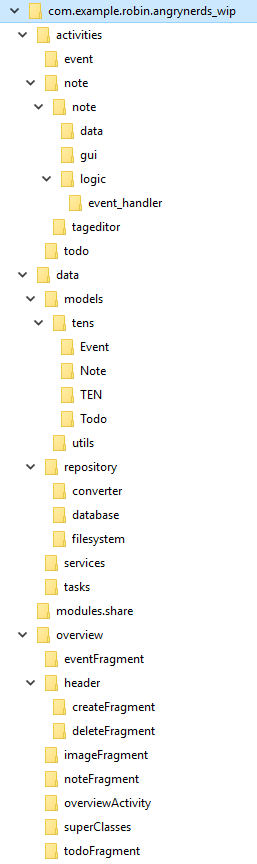
\includegraphics[width=5.5cm]{img/Projektordnerstruktur}\\ % Pfad
\source{Erstellt von Sertan Cetin} % Quelle
\end{minipage}
\end{figure}

Das Paket beinhaltet insgesamt fünf Activities mit jeweils einer ApplicationLogic, Gui und Data.

\begin{figure}[H]
\centering
\begin{minipage}[t]{1\textwidth} % Breite, z.B. 1\textwidth		
\caption{Paketstruktur} % Überschrift
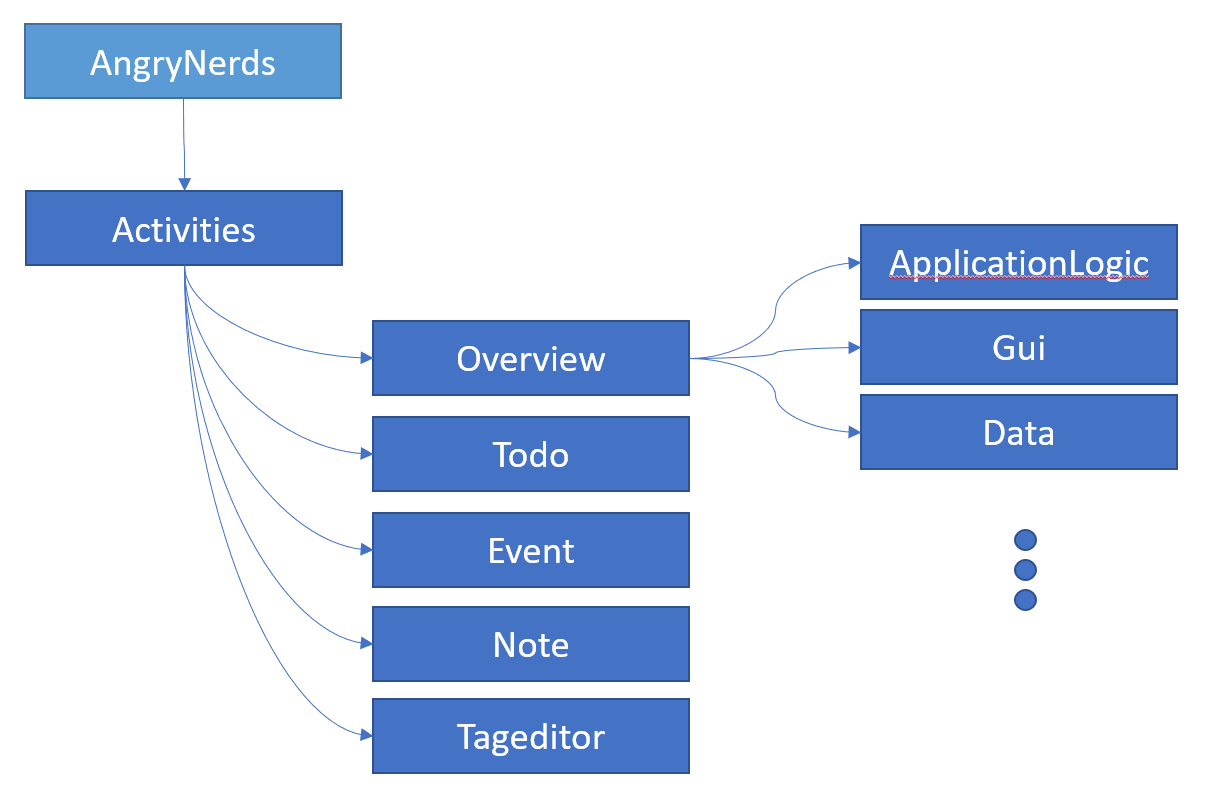
\includegraphics[width=1\textwidth]{img/Paketstruktur}\\ % Pfad
\source{Erstellt von Sertan Cetin} % Quelle
\end{minipage}
\end{figure}

\newpage
\subsection{Dokumentation der Activities}
%%%%%%%%%%%
%Alle
%%%%%%%%%%%

\subsubsection{Main Activity}
\fancyhead[L]{Main Activity}

%Yannick
\paragraph{Aufgabe und Funktionen (Yannick Rüttgers)}
Die in diesem Kapitel erläuterte Activity Overview dient dem Nutzer als Einstiegspunkt in die Applikation. Von hier aus werden alle weiteren Activities aufgerufen.

Wenn der Nutzer die Applikation startet, sieht er als erstes diese Activity. Diese enthält alle bereits erstellten TENs in Kachelform mit einigen Infos. Die Kacheln sind in einer oder mehreren Spalten, je nach Größe des Displays angeordnet. Diese Kacheln sind scrollbar.

Am unteren Bildschirmrand hat der Nutzer die Möglichkeit, sich nur die Kacheln, die zu einer der verschiedenen TEN-Arten gehören, anzeigen zu lassen. Dazu gibt es vier Buttons, die die jeweiligen TEN-Arten und eine generelle Übersicht über alle TENs darstellen.

Am oberen Bildschirmrand kann der Nutzer die einzelnen TEN-Arten neu erstellen, oder eine Suche öffnen. Auch hier sind wieder Buttons zu finden.

Der Nutzer hat die Möglichkeit, über ein langes gedrückt halten einer Kachel, in den Löschmodus zu gelangen. Hier können dann multiple Kacheln markiert werden und über ein neues Menü am oberen Bildschirmrand gelöscht werden.

Weitere Infos und Screenshots zum Layout der Applikation sind im nachfolgenden Kapitel zu finden.

Da die Activity als Einstiegspunkt in die Applikation genutzt wird, müssen von hier aus alle weiteren Activities zu erreichen sein. Die weiteren Activities umfassen die Anzeige und Neuerstellung von TENs. Die Erreichung dieser geschieht über die vorhin genannten Buttons und über die Kacheln.

Die Activity selbst besteht aus einer Oberfläche mit den genannten Buttons. Die einzelnen TENs werden mithilfe von Fragments eingefügt. Für jede TEN-Art gibt es ein eigenes Fragment. Diese Fragments bestehen aus mehreren Klassen. Der genaue Aufbau dieser wird später erläutert. Um mit den Fragments arbeiten zu können, verfügt die Activity über verschiedene Helferklassen, um diesen Prozess zu strukturieren.


%Fabia
\paragraph{Layouts, Screenshots (Fabia Schmid)}
Das Layout der Overview Activity orientiert sich an dem vorher erstellten Mockup und besteht aus drei Grundkomponenten. Es gibt am oberen Bildschirmrand eine Leiste zum Erstellen von Notes, Events und ToDos, sowie ein Button zum Suchen. Unter dieser leiste befindet sich ein Container, welcher die verschiedenen Fragments der vorhandenen Notes, Events und ToDos beinhaltet. Am unteren Bildschirmrand befindet sich noch eine Leiste mit vier Buttons zum Filtern der  Fragments (vgl. Abbildung Overview Activity).

Die obere Leiste ist ein RelativeLayout, welches eine TextView und drei Button beinhaltet. Diese ist ein gesondertes Fragment, damit der Wechsel zu einer anderen Leiste, z.B. bei dem Löschvorgang, vereinfacht wird. Darunter ist eine ScrollView, die es ermöglicht, dass durch die Fragments gescrollt werden kann. In der ScrollView befinden sich LinearLayouts, die mit den Fragments befüllt werden können. Die untere Leiste besteht abschließend aus einem LinearLayout, welches horizontal ausgerichtet ist und vier Buttons beinhaltet, mit denen gefiltert werden kann.

\begin{figure}[H]
\centering
\begin{minipage}[t]{1\textwidth} % Breite, z.B. 1\textwidth		
\caption{Overview Activity} % Überschrift
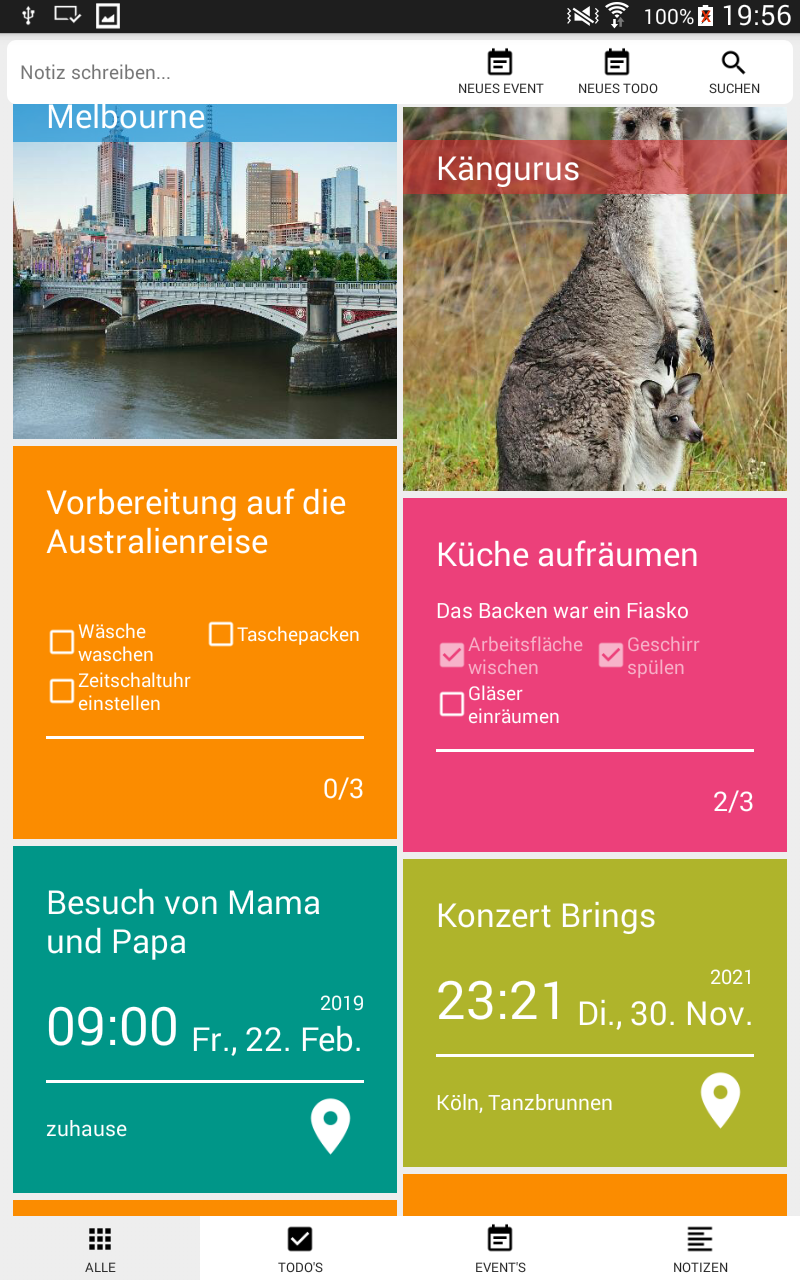
\includegraphics[height=20cm]{img/Overview}\\ % Pfad
\source{Screenshot aus der Benutzeroberfläche} % Quelle
\end{minipage}
\end{figure}

Die Activity Overview zeigt normal 2 Spalten mit Fragments, wenn jedoch das Tablet gedreht wird zeigt die Landscape-Ansicht drei Spalten mit Fragments, um den Bildschirm optimal zu nutzen (vgl. Abbildung Landscape-Ansicht Overview Activity).

\begin{figure}[H]
\centering
\begin{minipage}[t]{1\textwidth} % Breite, z.B. 1\textwidth		
\caption{Landscape Ansicht - Overview Activity} % Überschrift
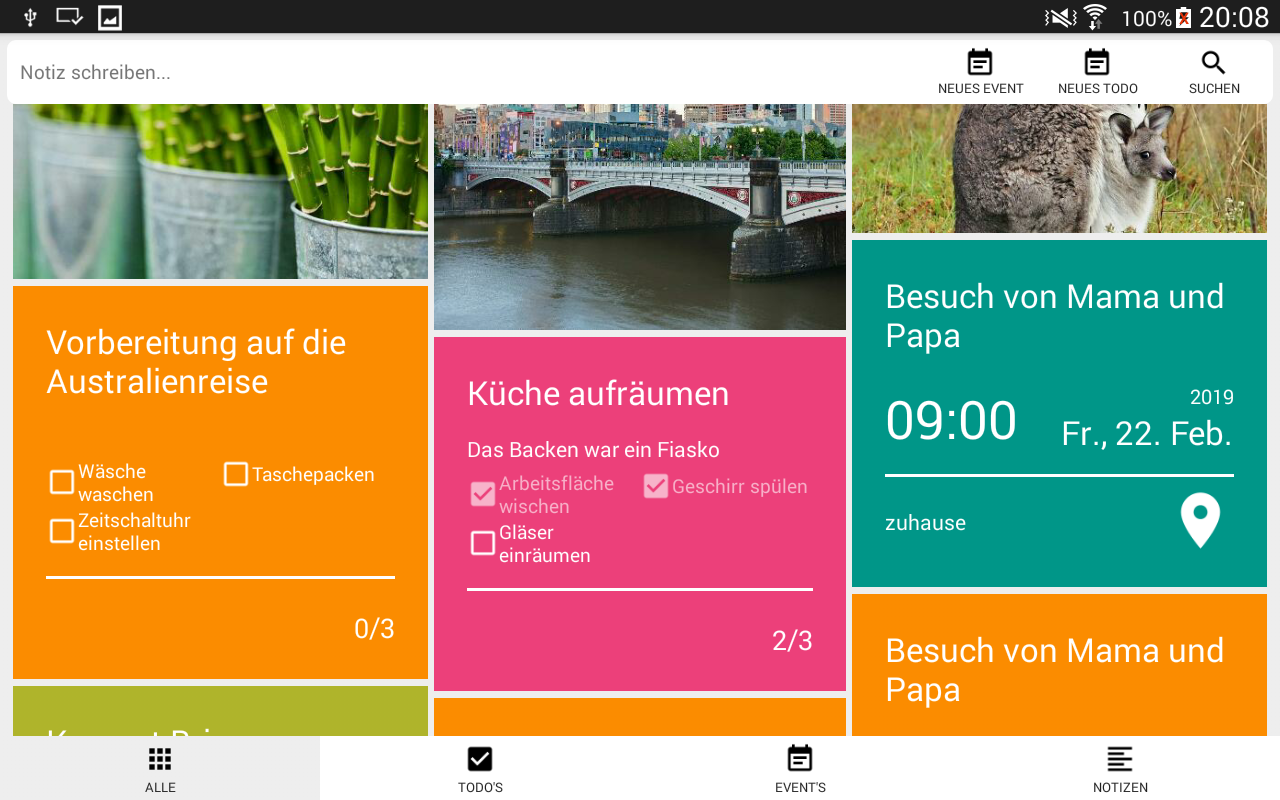
\includegraphics[width=1\textwidth]{img/Landscape}\\ % Pfad
\source{Screenshot aus der Benutzeroberfläche} % Quelle
\end{minipage}
\end{figure}

Die drei verschiedenen Arten von Fragments sind Notes, ToDo und Event.

Bei einer Note wird die Überschrift und ein Textauszug angezeigt. Wenn jedoch ein Bild in der Notiz vorhanden ist wird dieses mit der Überschrift in der Overview Activity angezeigt (vgl. Abbildung Note Fragments).

\begin{figure}[H]
\centering
\begin{minipage}[t]{1\textwidth} % Breite, z.B. 1\textwidth		
\caption{Note Fragments} % Überschrift
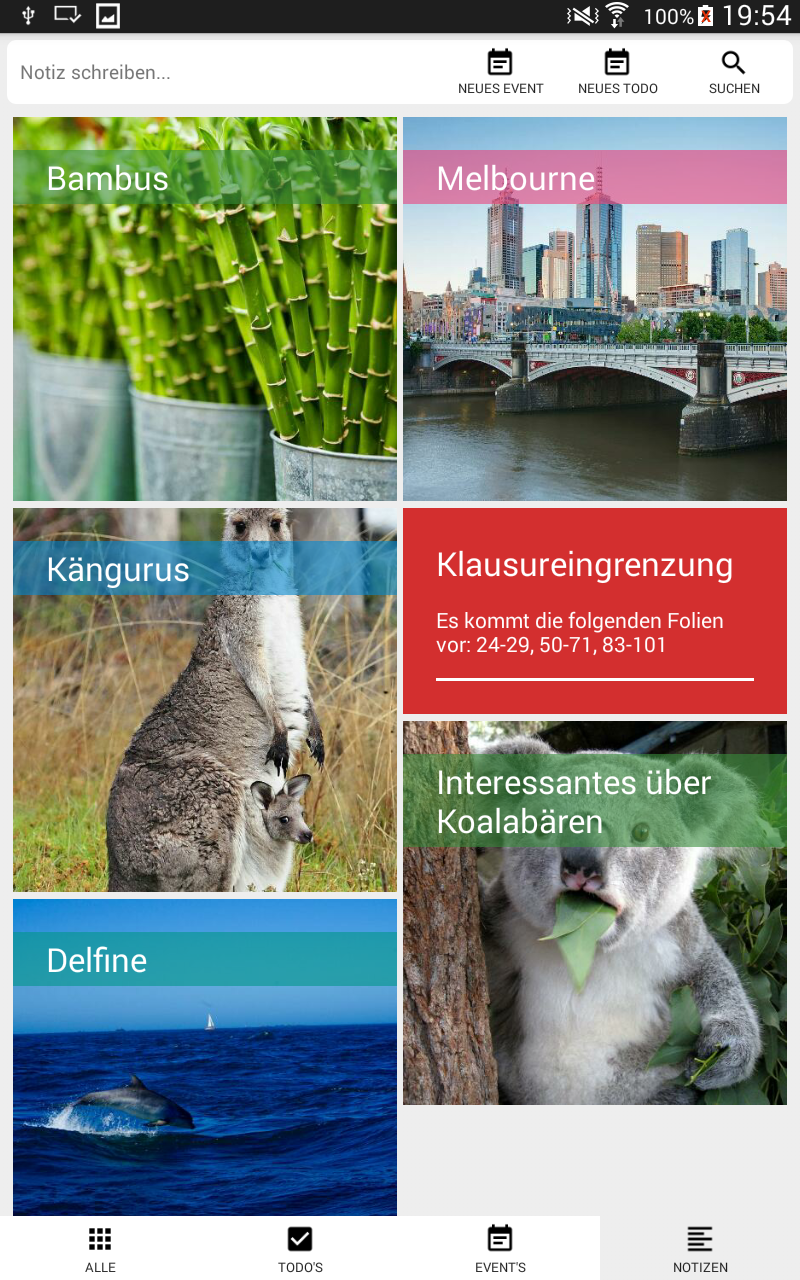
\includegraphics[height=17cm]{img/FragmentN}\\ % Pfad
\source{Screenshot aus der Benutzeroberfläche} % Quelle
\end{minipage}
\end{figure}

Die Fragments für die ToDos, zeigen auch den Titel an und die einzelnen Aufgaben mit Kästchen, die mit einem Hacken gefüllt sind, wenn sie erledigt sind. Zusätzlich wird Angezeigt, wie viele Aufgaben schon erfüllt wurden (vgl. Abbildung ToDo Fragments).

\begin{figure}[H]
\centering
\begin{minipage}[t]{1\textwidth} % Breite, z.B. 1\textwidth		
\caption{Todo Fragments} % Überschrift
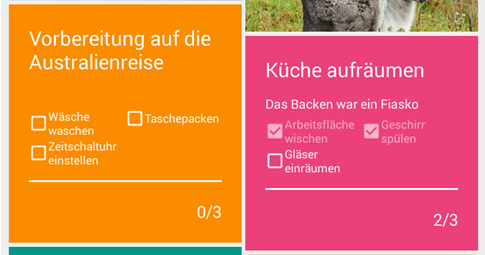
\includegraphics[width=1\textwidth]{img/FragmentT}\\ % Pfad
\source{Screenshot aus der Benutzeroberfläche} % Quelle
\end{minipage}
\end{figure}

Die Event Fragmentes bestehen aus der Überschrift, dem Datum und der Uhrzeit, sowie aus einem Ort, der angegeben werden kann (vgl. Abbildung Event Fragments).

\begin{figure}[H]
\centering
\begin{minipage}[t]{1\textwidth} % Breite, z.B. 1\textwidth		
\caption{Event Fragments} % Überschrift
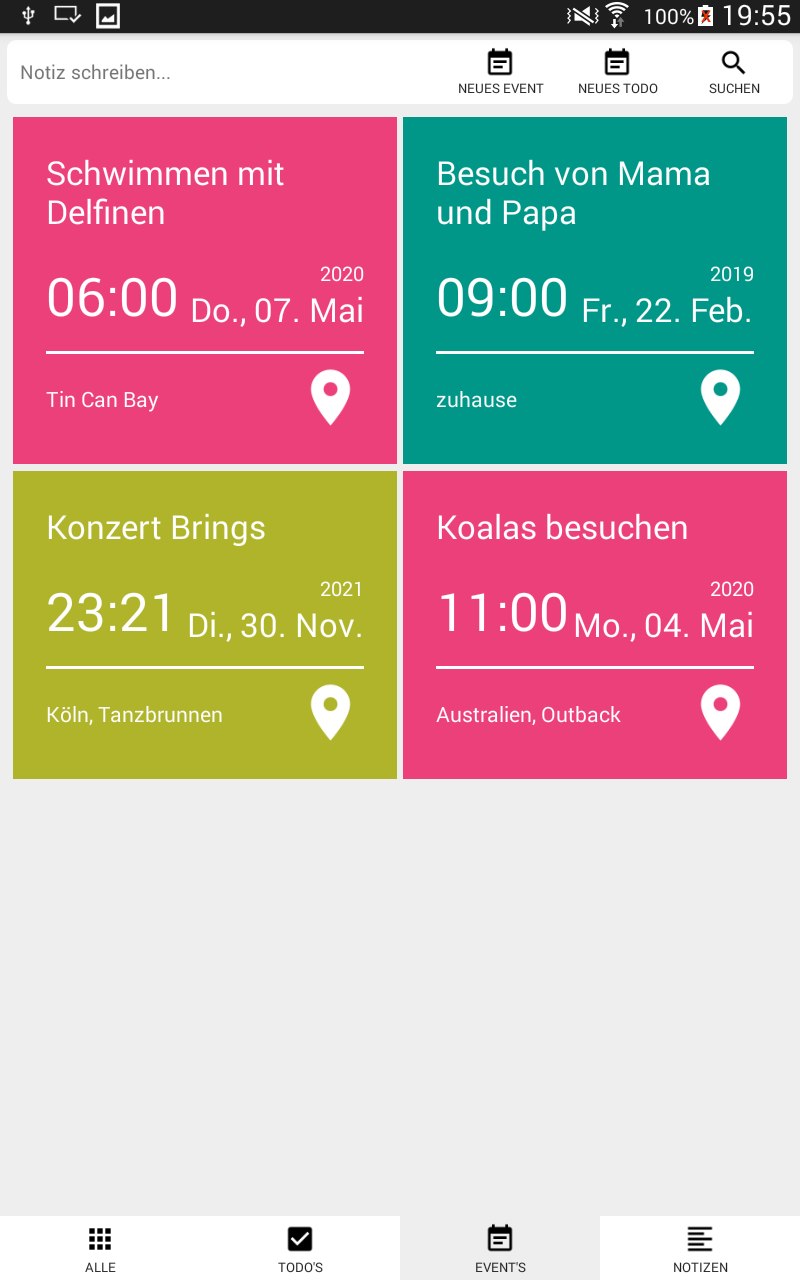
\includegraphics[height=17cm]{img/FragmentE}\\ % Pfad
\source{Screenshot aus der Benutzeroberfläche} % Quelle
\end{minipage}
\end{figure}

In der Overview Activity kann zusätzlich gesucht und gelöscht werden. Wenn man einen langen Click auf ein Fragment macht, wird die obere Leiste verändert und man bekommt einen Button zum Löschen. Dies ist dadurch möglich, dass die obere Leiste ein Fragment ist. Zusätzlich kann in dieser Ansicht nun auf die verschiedenen Fragments geklickt werden, um diese zu markieren und mehrere gleichzeitig zu löschen. Markierungen werden mittels einem Hacken gekennzeichnet. Diese Ansicht kann durch den Zurück-Pfeil verlassen werden (vgl. Abbildung Overview Activity Löschen).

\begin{figure}[H]
\centering
\begin{minipage}[t]{1\textwidth} % Breite, z.B. 1\textwidth		
\caption{Overview Activity - Löschen} % Überschrift
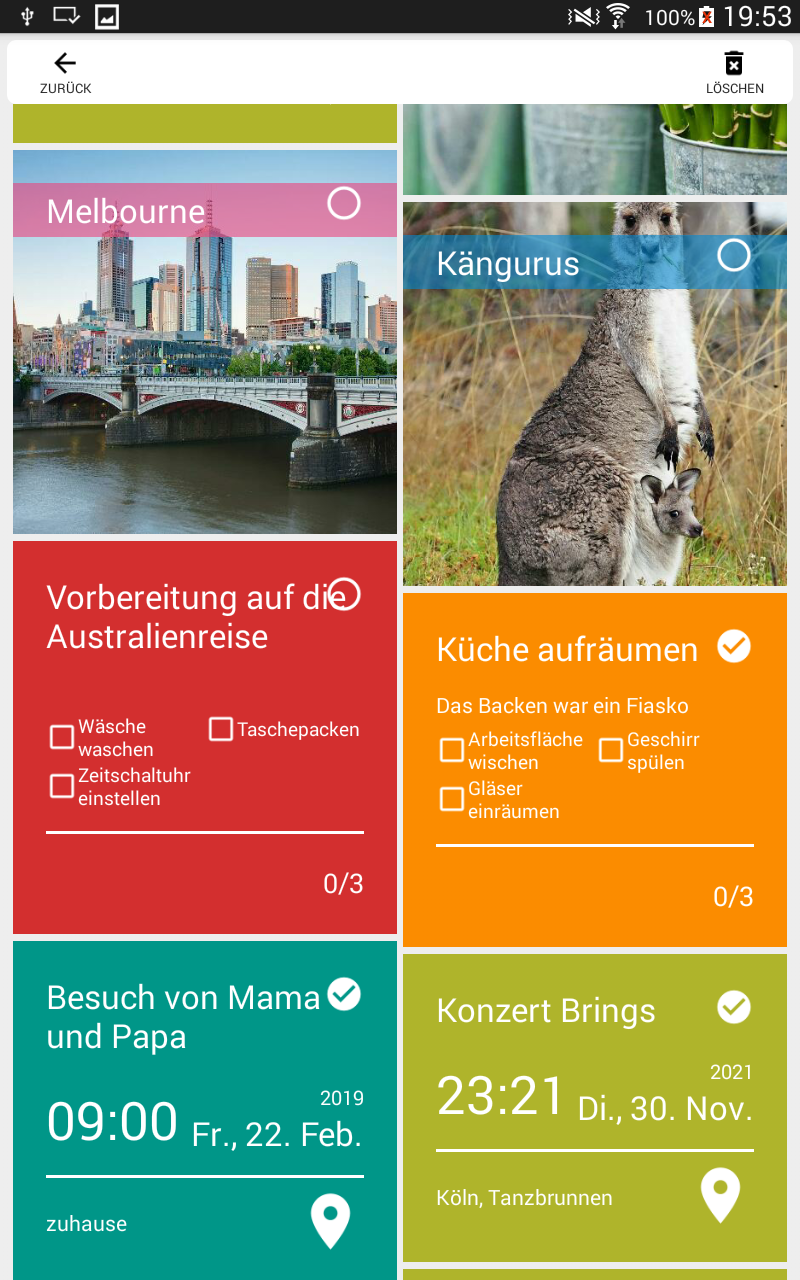
\includegraphics[height=17cm]{img/Loeschen}\\ % Pfad
\source{Screenshot aus der Benutzeroberfläche} % Quelle
\end{minipage}
\end{figure}

Auch bei der Suchfunktion wird die obere Leiste angepasst. Auch hier möglich durch das Fragment. Dabei kann nun ein beliebiges Wort eingegeben werden, welches in den verschiedenen Einträgen gesucht wird. Die gefundenen Einträge werden daraufhin angezeigt. Um die Suche zu beenden kann der Zurück-Pfeil verwendet werden (vgl. Abbildung Overview Activity Suchen).

\begin{figure}[H]
\centering
\begin{minipage}[t]{1\textwidth} % Breite, z.B. 1\textwidth		
\caption{Overview Activity - Suchen} % Überschrift
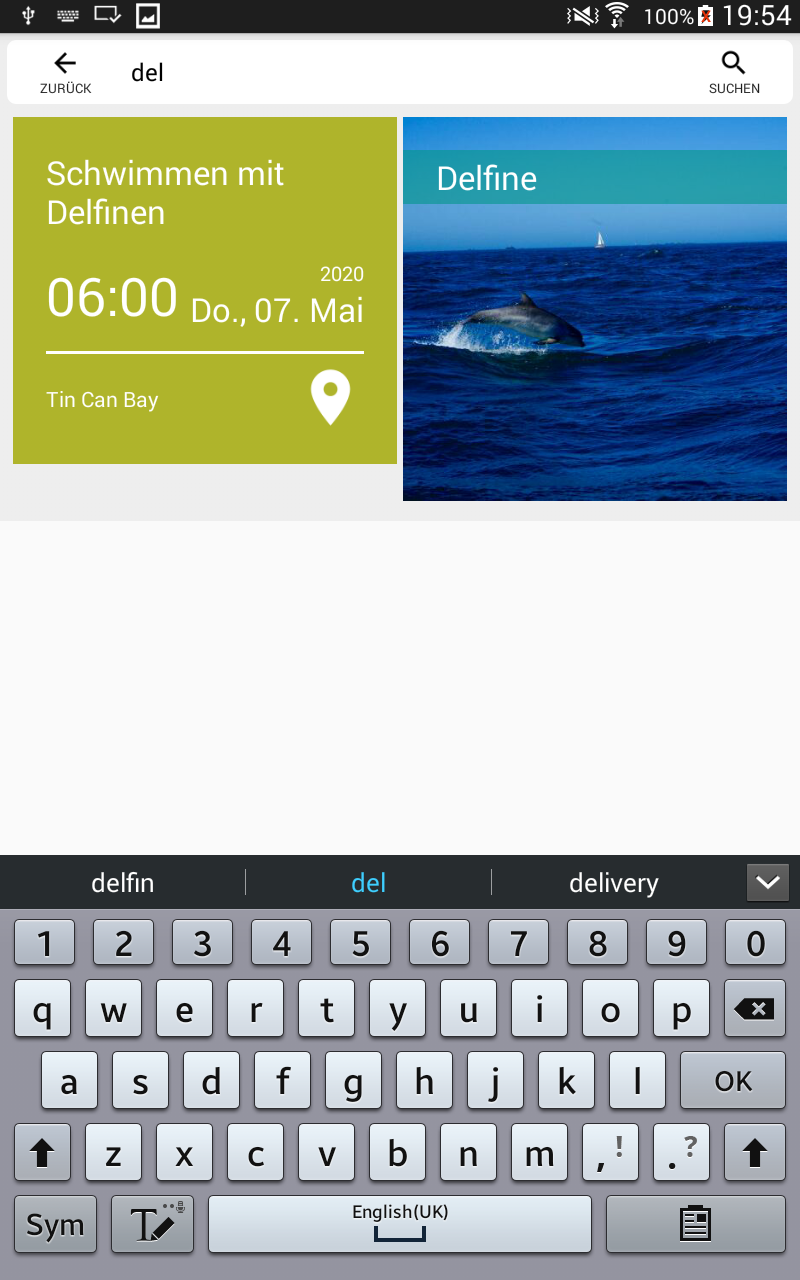
\includegraphics[height=17cm]{img/Suchen}\\ % Pfad
\source{Screenshot aus der Benutzeroberfläche} % Quelle
\end{minipage}
\end{figure}

%Yannick
\paragraph{Use Case (Yannick Rüttgers)}
Wie bereits geschrieben, dient diese Activity dem Nutzer als Einstiegspunkt in die Applikation. Hier kann er einige Aktionen durchführen.
 
Zum einen kann er die Oberfläche der Übersicht selbst beeinflussen. Hierzu gibt es am unteren Bildschirmrand einige Buttons, mit denen er nach den verschiedene TEN-Arten filtern kann. Zusätzlich kann er über eine Suchfunktion alle TENs durchsuchen.

Aus dieser Activity heraus können vom User auch neue TENs erstellt werden. Hierzu wird er allerdings an weitere Activities weitergeleitet.

Zuletzt ist es dem Nutzer auch möglich, mehrere TENs auf einmal zu löschen. Dies geschieht, wie bereits gesagt, über ein markieren einzelner Kacheln.

Im Folgenden ist das Usecase-Diagramm für die Übersicht zu sehen.

\begin{figure}[H]
\centering
\begin{minipage}[t]{1\textwidth} % Breite, z.B. 1\textwidth		
\caption{Usecase Diagramm der Overview} % Überschrift
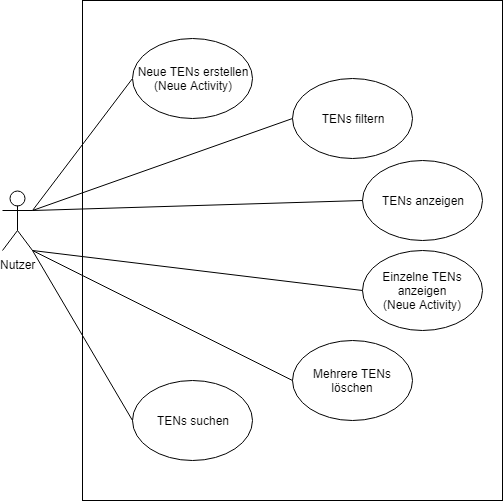
\includegraphics[width=1\textwidth]{img/Usecase_Overview}\\ % Pfad
\source{Erstellt von Yannick Rüttgers} % Quelle
\end{minipage}
\end{figure}

%Yannick
\paragraph{Datenstruktur und Typen (Yannick Rüttgers)}
Die Daten für diese Activity werden hauptsächlich über die Klasse OverviewData verwaltet.

Wenn die Activity initiiert wird, werden zuerst alle nötigen Instanzen erstellt. Hierzu gehört unter anderen eine Instanz der Klasse OverviewData. Diese Klasse ruft in ihrem Konstruktor mithilfe einer statischen Servicemethode alle TENs als Objekte ab. Diese Objekte werden in einer ArrayList gespeichert. Bei Bedarf werden diese Daten neu geladen.

Um beim Suchen oder Filtern nicht alle Daten neu laden zu müssen, gibt es eine weitere ArrayList, die immer den gefilterten Datenstand enthält. Aus diesen Daten werden die Fragments generiert.

Um die Filterung von Fragments beim Wechsel der Orientierung der Applikation beibehalten zu können, wird dies ebenfalls im Dataobjekt hinterlegt.

Wenn Fragments generiert werden, bekommen diese die Daten des zugehörigen TEN-Objekts als Bundle mitgegeben. Während der Initialisierung jedes Fragments, werden die Daten im jeweiligen Data Objekt abgelegt. Die Parameter dieser Dataobjekte bilden zum größten Teil die der TEN-Objekte ab. Im Konstruktor der Dataklasse werden den einzelnen Parametern dann die Werte aus dem Bundle zugewiesen. Da in der Activity die TENs nicht bearbeitet werden können, gibt es im Nachhinein keine Möglichkeit den Fragments neue Daten zuzuweisen.

Zusätzlich hält jedes Fragment zwei Informationen über sich. Dies ist zum einen der Löschzustand, über den das Fragment steuern kann, ob es zum Löschen markiert werden kann oder nicht. Zum anderen hält das Fragment die Information, ob es markiert ist, um dies im Falle einer Löschung angeben zu können. Diese beiden Informationen können aus dem Fragment abgerufen werden.

%Yannick
\paragraph{Dokumentation des Quelltextes der Activity (Yannick Rüttgers)}

\subparagraph{Allgemein}

Die OverviewActivity besteht aus 35 verschiedenen Klassen. Diese Klassen sind in verschiedene Pakete unterteilt.

Zum einen gibt es die Klassen, die unmittelbar zur OverviewActivity an sich gehören. Zu diesen zugehörig sind die Klassen, die für den Header der Activity genutzt werden.

Alle weiteren Klassen werden für die Fragments, die die TENs darstellen, genutzt. Hierzu gibt es vier Superklassen und zwei Listener, die in allen Fragments genutzt werden. Jedes der vier verschiedenen Fragments hat nochmal vier weitere Klassen, die von den Superklassen erben.
In Folgender Grafik soll dies verdeutlicht werden.

\begin{figure}[H]
\centering
\begin{minipage}[t]{1\textwidth} % Breite, z.B. 1\textwidth		
\caption{Klassendiagramm} % Überschrift
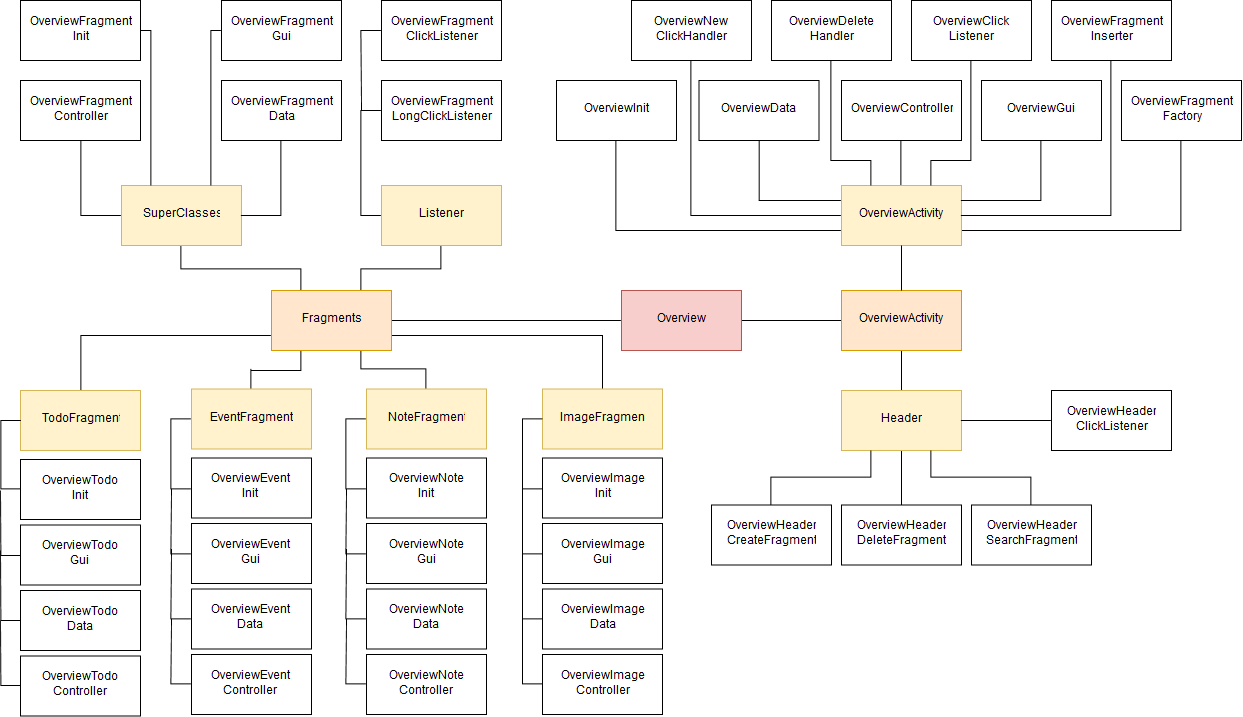
\includegraphics[height=20cm]{img/Klassendiagramm_lite}\\ % Pfad
\source{Erstellt von Yannick Rüttgers} % Quelle
\end{minipage}
\end{figure}

Die Funktion der Klassen und wichtige Methoden werden im Folgenden erläutert.

\subparagraph{Activityklassen}

Zu den Klassen, die unmittelbar zur Activity gehören, zählen neun verschiedene Klassen.

\subparagraph*{Klasse: class OverviewInit extends AppCompatActivity}

Diese Klasse ist für die Initialisierung der verschiedenen Komponenten der Activity zuständig. Da sie von der Superklasse AppCompatActivity erbt, implementiert sie zusätzlich die Methoden des Activitylifecycles.

Wichtige Methoden:

\textit{-protected void OnCreate(Bundle savedInstanceState)}

Diese Methode ist eine der Lifecyclemethoden von Activities, sie wird beim entstehen der Activity aufgerufen. Hier werden die verschiedenen Komponenten der Activity mit den zugehörigen Methoden initiiert.

\textit{-public void onConfigurationChanged(Configuration newConfig)}

Diese Methode wird aufgerufen, wenn sich etwas an der Konfiguration der Applikation ändert, wie in diesem Fall die Ausrichtung des Gerätes. Hier werden der Controller und die Gui neu initiiert. Dazu werden die Methoden initGui() und initController() aufgerufen.

\subparagraph*{Klasse: class OverviewData}

Diese Klasse ist für die Datenhaltung innerhalb der Activity verantwortlich. Hier befinden sich auch die zum Sortieren und zum Suchen verwendeten Methoden. Initial werden die Daten einmal geladen, bei Bedarf werden diese über eine Methode neugeladen. Die Daten werden dabei zweimal gehalten: Eine Liste enthält alle TENs, die andere Liste enthält die TENs, die angezeigt werden sollen.

Wichtige Methoden:

\textit{-public void refresh()}

Läd die Daten neu.

\textit{-public ArrayList<TEN> filterData()}

Filtert die Daten nach dem aktuell ausgewählten TEN-Typen.

\textit{-public void search(String pSearchString)}

Fügt nur die Suchergebnisse in die Liste der TENs ein, die angezeigt werden sollen.

\subparagraph*{Klasse: class OverviewGui}

Diese Klasse verwaltet die Benutzeroberfläche der Activity.

Wichtige Methoden:

\textit{-public void markButton(Class pClass)}

Markiert einen der Buttons am unteren Bildschirmrand, je nachdem welcher TEN-Typ ausgewählt ist.

\textit{-public void showFooter() / hideFooter()}

Zeigt oder versteckt die Buttons am unteren Bildschirmrand.

\subparagraph*{Klasse: class OverviewController}

Diese Klasse verwaltet die einzelnen Helferklassen und stellt die Logik der Activity da. 

Wichtige Methoden:

In der Klasse wird die Suche aktiviert, sowie das Löschen von TENs verwaltet. Hierzu werden die Helferklassen OverviewDeleteHandler, OverviewNewClickHandler, OverviewFragmentFactory und OverviewFragmentInserter genutzt. 

\subparagraph*{Klasse: class OverviewFragmentFactory}

Diese Klasse erstellt verschiedene Arten von Fragments, die dann später genutzt werden können.

Wichtige Methoden:

\textit{-public Fragment createHeader(Create/Delete/Search)Fragment()}

Diese Methode liefert das gewählte Headerfragment zurück.

\textit{-public ArrayList<Fragment> createTENFragments(ArrayList<TEN> pTENs)}

Erstellt eine Liste von Fragments, die aus den TENs erstellt werden. Je nach Art des TENs wird ein unterschiedliches Fragment erstellt.

\subparagraph*{Klasse: class OverviewFragmentInserter}

Diese Klasse fügt Fragments in die Benutzeroberfläche ein. Hierzu wird der FragmentManager der Activity genutzt.

Wichtige Methoden:

\textit{-public void insertFragment(int pContainerID, Fragment pFragment, String pTag)}

Fügt ein Fragment in einen gewählten Container ein. Dem Fragment wird ein Tag zugewiesen.

\textit{-public void replaceFragment(int pContainerID, Fragment pFragment, String pTag)}

Ersetzt ein Fragment in einem gewählten Container durch ein anderes. Dem Fragment wird ein Tag zugewiesen.

\textit{-public void insertFragments(int[] pContainerIDs, ArrayList<Fragment pFragments)}

Fügt eine beliebige Anzahl Fragments in eine beliebige Anzahl Container an. Dabei werden die Container zyklisch durchlaufen.

\subparagraph*{Klasse: class OverviewClickListener}

Diese Klasse verwaltet die Klickevents der OverviewActivity. Je nach geklicktem Button wird eine andere Methode des Controllers aufgerufen.

Wichtige Methoden:

\textit{-public void onClick(View view)}

Ruft je nach angeklickter View die show()-Methode des Controllers mit einem bestimmten Parameter auf.

\subparagraph*{Klasse: class OverviewDeleteHandler}

Diese Klasse verwaltet die Methoden, die zum Löschen beziehungsweise nicht Löschen von TENs nötig sind.

Wichtige Methoden:

\textit{-public void longClick()}

Aktiviert den Löschvorgang für alle Fragments.

\textit{-public void back()}

Deaktiviert den Löschvorgang für alle Fragments.

\textit{-public void delete()}

Sammelt alle markierten Fragments und löscht die dazugehörigen TENs. Deaktiviert den Löschvorgang für alle anderen Fragments.

\subparagraph*{Klasse: class OverviewNewClickHandler}

Verwaltet das Erstellen von neuen TENs.

Wichtige Methoden:

\textit{-public void newTEN(Class pClass)}

Startet eine neue Activity, je nachdem welche TEN-Art angegeben wurde.

\subparagraph{Header}

Die Header der Activity sind wechselnde Fragments, die verschiedene Aufgaben haben. Sie werden am oberen Bildschirmrand ausgetauscht. Ein Fragment dient dem Neuerstellen von TENs, eines das Löschen und eines das Suchen.

Die Fragments teilen sich einen ClickListener.

\subparagraph*{Klasse: class OverviewHeaderCreateFragment}

Dieses Fragment dient dazu, das Erstellen von neuen TENs anzustoßen. Hierzu enthält es drei Buttons. Zusätzlich gibt es einen Button zum Starten der Suche.

\subparagraph*{Klasse: class OverviewHeaderDeleteFragment}

Dieses Fragment dient dem Löschvorgang. Es gibt einen Button zum Abbrechen des Prozesses und einen Button, um die Löschung durchzuführen.

\subparagraph*{Klasse: class OverviewHeaderSearchFragment}

Dieses Fragment dient dem Suchvorgang. Es gibt ein Textfeld, in das ein Suchbegriff eingegeben werden kann. Außerdem gibt es einen Button zum Abbrechen des Prozesses und einen, um die Suche durchzuführen.

\subparagraph*{Klasse: class OverviewHeaderClickListener}

Diese Klasse behandelt die Clickevents der Headerfragments. Je nachdem, welcher Button in einem der Fragments geklickt wurde, wird eine andere Methode im Controller aufgerufen.

Wichtige Methoden:

\textit{-public void onClick(View view)}

Diese Methode wird ausgeführt, sobald einer der Buttons eines Headers geklickt wird. Je nachdem, welcher Button dies war, wird eine Methode im Controller aufgerufen.

\subparagraph{Superklassen}

Die folgenden Klassen dienen als Superklassen für die Fragments. Dies wurde so entwickelt, da alle vier Fragments sich ähnliche Funktionen teilen. Große Teile der Implementierung nutzen außerdem die Polymorphie.

\subparagraph*{Klasse: class OverviewFragmentInit}

Diese Klasse dient als Superklasse für die Initialklassen der einzelnen Fragments. Hier werden die anderen drei Komponenten der Fragments initialisiert. Ausserdem werden zum Start des Fragments mehrere andere Methoden aufgerufen.

Wichtige Methoden:

\textit{-public void onCreateView(Bundle pArguments, View pView)}

Diese Methode startet, wenn das Fragment erstellt wird, verschiedene Methoden des Controllers.

\subparagraph*{Klasse: class OverviewFragmentData}

Diese Klasse dient als Superklasse für die Dataklassen der einzelnen Fragments. Sie bildet die Klasse TEN nach.

Wichtige Methoden:

\textit{-public void addData(Bundle pData)}

Diese Methode pflegt die Daten aus einem Bundle in das Objekt ein.

\subparagraph*{Klasse: class OverviewFragmentGui}

Diese Klasse dient als Superklasse für die Guiklassen der einzelnen Fragments. Sie kümmert sich um den Markierungsprozess der Fragments für den Löschvorgang.

Wichtige Methoden:

\textit{-public void applyMarked(boolean pMarked)}

Diese Methode setzt den Zustand des Checkboxicons auf den des übergebenen Zustandes.

\subparagraph*{Klasse: class OverviewFragmentController}

Diese Klasse dient als Superklasse für die Controllerklassen der einzelnen Fragments. Hauptsächlich wird sich auch hier um den Löschprozess gekümmert, da dieser für alle Fragments gleich ist.

Wichtige Methoden:

\textit{-public void longClicked()}

Diese Methode startet den Löschprozess. Dazu wird der Controller der Activity, die das Fragment verwaltet aufgerufen, und ihm mitgeteilt, dass der Löschprozess gestartet werden soll.

\subparagraph{Listener}

\subparagraph*{Klasse: class OverviewFragmentClickListener}

Diese Klasse ist dafür zuständig, dass, wenn ein Fragment angeklickt wird, im Controller dieses Fragments eine Methode ausgeführt wird. So wird eines der Fragments geöffnet.

\subparagraph*{Klasse: class OverviewFragmentLongclickListenerFragment}

Diese Klasse ist dafür zuständig, dass, wenn ein Fragment lange angeklickt wird, die entsprechende Methode im Controller des Fragments aufgerufen wird. So gelangt der Nutzer in den Löschvorgang.

\subparagraph{Fragments Allgemein}

Die folgenden Kapitel behandeln die vier genutzten Fragments. Alle Fragments erben von den vier zuvor genannten Superklassen, und teilen sich so eine Struktur. Zudem wird, um den Quellcode übersichtlich zu halten, viel Wert auf die Nutzung von Polymorphie gelegt.

\subparagraph{TodoFragment}

Die folgenden Klassen implementieren das Fragment, welches die Todos abbildet.

\subparagraph*{Klasse: class OverviewTodoInit}

Diese Klasse initiiert alle nötigen Komponenten für das Todo-Fragment.

\subparagraph*{Klasse: class OverviewTodoData}

Diese Klasse stellt die Datenhaltung für das Todo-Fragment dar. Sie bildet die Klasse Todo nach.

Wichtige Methoden:

\textit{-public void addData(Bundle pData)}

Diese Methode pflegt die Daten aus einem Bundle in das Objekt ein.

\subparagraph*{Klasse: class OverviewTodoGui}

Diese Klasse verwaltet die GUI für das Todo-Fragment. Hier geschieht auch die Generierung der Checkboxen aus den Todo-Tasks.

Wichtige Methoden:

\textit{-public void addView(View pView)}

Diese Methode fügt die View des Fragments dem Objekt hinzu. Außerdem werden den Attributen Views zugewiesen.

\textit{-public void addCheckbox(boolean pStatus, String pDescription)}

Fügt dem Fragment eine Checkbox hinzu, die aus einem Kästchen und einer Beschreibung besteht.

\subparagraph*{Klasse: class OverviewTodoController}

Diese Klasse stellt die Logik des Todofragments dar. Hier werden den Feldern der Benutzeroberfläche Werte zugewiesen. Zusätzlich werden aus den Tasks des Todos Checkboxen generiert.

\textit{-public void applyData()}

Diese Methode übergibt die Attribute des Dataobjekts an das Guiobjekt, damit die Views aktualisiert werden können.

\textit{-public void generateCheckboxes()}

Diese Methode generiert aus der Taskliste des Todos mithilfe der addCheckbox-Methode des Guiobjekts Checkboxen.

\subparagraph{EventFragment}

Die folgenden Klassen implementieren das Fragment, welches die Events abbildet.

\subparagraph*{Klasse: class OverviewEventInit}

Diese Klasse initiiert alle nötigen Komponenten für das Event-Fragment.

\subparagraph*{Klasse: class OverviewEventData}

Diese Klasse stellt die Datenhaltung für das Event-Fragment dar. Sie bildet die Klasse Event nach. Hier wird das Kalenderobjekt in seine Einzelteile zerlegt.

Wichtige Methoden:

\textit{-public void addData(Bundle pData)}

Diese Methode pflegt die Daten aus einem Bundle in das Objekt ein.

\subparagraph*{Klasse: class OverviewEventGui}

Diese Klasse verwaltet die GUI für das Event-Fragment.

Wichtige Methoden:

\textit{-public void addView(View pView)}

Diese Methode fügt die View des Fragments dem Objekt hinzu. Außerdem werden den Attributen Views zugewiesen.

\subparagraph*{Klasse: class OverviewEventController}

Diese Klasse stellt die Logik des Eventfragments dar. Hier werden den Feldern der Benutzeroberfläche Werte zugewiesen.

\textit{-public void applyData()}

Diese Methode übergibt die Attribute des Dataobjekts an das Guiobjekt, damit die Views aktualisiert werden können.

\subparagraph{NoteFragment}

Die folgenden Klassen implementieren das Fragment, welches die Notes abbildet, die keine Bilder haben.

\subparagraph*{Klasse: class OverviewNoteInit}

Diese Klasse initiiert alle nötigen Komponenten für das Note-Fragment.

\subparagraph*{Klasse: class OverviewNoteData}

Diese Klasse stellt die Datenhaltung für das Note-Fragment dar. Sie bildet die Klasse Note nach.

Wichtige Methoden:

\textit{-public void addData(Bundle pData)}

Diese Methode pflegt die Daten aus einem Bundle in das Objekt ein.

\subparagraph*{Klasse: class OverviewNoteGui}

Diese Klasse verwaltet die GUI für das Note-Fragment.

Wichtige Methoden:

\textit{-public void addView(View pView)}

Diese Methode fügt die View des Fragments dem Objekt hinzu. Außerdem werden den Attributen Views zugewiesen.

\subparagraph*{Klasse: class OverviewNoteController}

Diese Klasse stellt die Logik des Note-Fragments dar. Hier werden den Feldern der Benutzeroberfläche Werte zugewiesen.

\textit{-public void applyData()}

Diese Methode übergibt die Attribute des Dataobjekts an das Guiobjekt, damit die Views aktualisiert werden können.

\subparagraph{ImageFragment}

Die folgenden Klassen implementieren das Fragment, welches die Notes abbildet, in denen Bilder gespeichert wurden.

\subparagraph*{Klasse: class OverviewImageInit}

Diese Klasse initiiert alle nötigen Komponenten für das Image-Fragment.

\subparagraph*{Klasse: class OverviewImageData}

Diese Klasse stellt die Datenhaltung für das Image-Fragment dar. Hier wird das Previewimage für die Notiz geladen.

Wichtige Methoden:

\textit{-public void addData(Bundle pData)}

Diese Methode pflegt die Daten aus einem Bundle in das Objekt ein und läd das Previewimage.

\subparagraph*{Klasse: class OverviewImageGui}

Diese Klasse verwaltet die GUI für das Image-Fragment.

Wichtige Methoden:

\textit{-public void addView(View pView)}

Diese Methode fügt die View des Fragments dem Objekt hinzu. Außerdem werden den Attributen Views zugewiesen.

\subparagraph*{Klasse: class OverviewImageController}

Diese Klasse stellt die Logik des Image-Fragments dar. Hier werden den Feldern der Benutzeroberfläche Werte zugewiesen.

\textit{-public void applyData()}

Diese Methode übergibt die Attribute des Dataobjekts an das Guiobjekt, damit die Views aktualisiert werden können.

\newpage
\subsubsection{Todo Activity}
\fancyhead[L]{Todo Activity}
%Florian
\paragraph{Aufgabe und Funktionen (Florian Rath)}
Die Activity Todo dient dem Nutzer dazu, seine Aufgaben zu organisieren. Wenn er eine neue Todo erstellt hat, hat er die Möglichkeit einen Titel und eine Beschreibung einzugeben. Diese Eingabemöglichkeiten sind jedoch optional und hindern den Nutzer nicht daran, die Todo wieder zu verlassen und somit abzuspeichern. Der Titel für eine Todo könnte beispielsweise „Einkaufsliste“ lauten, während die Beschreibung nähere Informationen wie zum Beispiel „Für die Geburtstagsparty von meiner Tochter“ beinhalten kann. So hat der Benutzer die Möglichkeit mehrere Einkaufslisten anzulegen und sie mit einer Beschreibung voneinander differenzieren.

Neben dem Titel und der Beschreibung können auch ein Start- und Enddatum festgelegt werden. Dies ist hilfreich, wenn für eine Todo bestimmte Fristen vorhanden sind. Geht es in der Todo z.B. um eine Prüfungsvorbereitung, kann der Benutzer auswählen, wann er spätestens mit dem Lernen anfangen muss und bis wann er spätestens mit dem Lernen Zeit hat. Diese Funktionalität ist ebenfalls optional. Man kann also auch Todos verwenden, ohne ein bestimmtes Start- und Enddatum anzugeben. Die App zeigt dann immer jeweils das aktuelle Datum in den Eingabefeldern an.

Die Hauptfunktionalität der Todo-Activity ist das Anlegen von sogenannten Tasks.- Eine Task besteht im Prinzip aus einem Text, wie z.B. „Luftballons“, und einem Status (boolean-Wert). Der Status gibt an, ob ein Task erledigt ist oder nicht. Dies geschieht über eine Checkbox, die neben jedem Task vorhanden ist.

Unterstrichen wird die Gesamtfunktionalität mit einer Fortschrittsanzeige. Ein prozentualer Wert gibt dabei an, wie viele Tasks als erledigt markiert sind. Wurden z.B. 5 von 10 Tasks als erledigt markiert, steht in der App 50 Prozent. Sind es hingegen 1 von 10 markierte, dann nur noch 10 Prozent. Diese Funktionalität dient dazu, dem Benutzer einen Fortschritt über seine Todo zu geben. Anhand des Fortschritts kann er sich nämlich organisieren, ob er in den genannten Fristen liegt. Liegt man kurz wenige Tage vor einer Prüfung gerade bei 10 Prozent, so könnte es langsam brenzlig für den Benutzer werden. Auch in einer sehr langen Liste von Tasks könnte dieser Wert nützlich sein. Da die Todo-Activity darauf ausgelegt ist, theoretisch endlos viele Tasks speichern zu können (so viele, wie ein ArrayList speichern kann), können sehr lange Listen entstehen. Unter hunderten von Tasks könnte es schnell passieren, eine unerledigte Aufgabe zu übersehen und die Todo verfrüht abzuschließen. Die App macht keine Obergrenze für Tasks, um dem User keine Arbeits- bzw. Organisationsweise vorzuschreiben.

Der User hat auch die Möglichkeit eine Todo zu löschen.

%Sertan
\paragraph{Layout, Screenshots (Sertan Cetin)}
Um eine maximale Bedienbarkeit zu gewährleisten, verfügt diese Activity insgesamt genau über zwei Layouts. Während das eine Layout die Benutzersteuerelement im Porträtmodus darstellt, dient das andere Layout dazu, die Elemente im Landscape-Modus darzustellen. Der Unterschied zwischen den beiden Layouts liegt in der Anordnung der Elemente. Im Porträtmodus belegt jedes Element eine Zeile auf dem Bildschirm. Sie sind also untereinander angeordnet. Im Landscape-Modus ist die Ansicht in zwei Spalten geteilt. In der linken Spalte sind der Titel, Beschreibung, Start- und Enddatum untereinander angeordnet. In der rechten Spalte befinden sich die einzelnen Aufgaben. Die Breite der linken Spalte hat einen festen Wert, nämlich 640px. Die Prozentanzeige befindet sich unabhängig von den beiden Spalten immer mittig am unteren Bildschirmrand.

Oben ist eine Toolbar vorhanden, mit einem Zurück-Button, um zur Hauptübersicht zu gelangen, und einem Menü, in welchem die Todo gelöscht werden kann.

Nachfolgender Screenshot zeigt den zuvor beschriebenen Landscape-Modus der Todo-Activity: 

\begin{figure}[H]
\centering
\begin{minipage}[t]{1\textwidth} % Breite, z.B. 1\textwidth		
\caption{Todo Activity im Landscape-Modus} % Überschrift
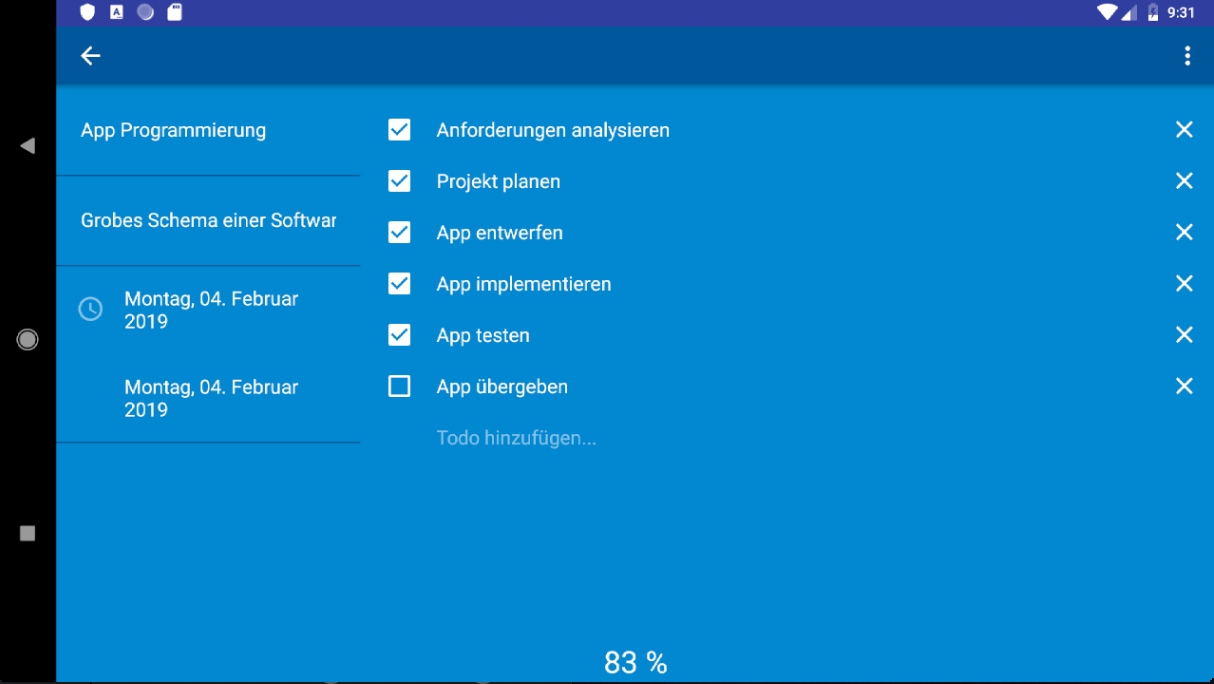
\includegraphics[width=1\textwidth]{img/Todo_landscape}\\ % Pfad
\source{Screenshot aus der Benutzeroberfläche} % Quelle
\end{minipage}
\end{figure}

Beim Wechsel der beiden Ansicht-Modi werden die Daten jeweils in das andere Layout übernommen.

\begin{figure}[H]
\centering
\begin{minipage}[t]{1\textwidth} % Breite, z.B. 1\textwidth		
\caption{Todo Activity im Portrait-Modus} % Überschrift
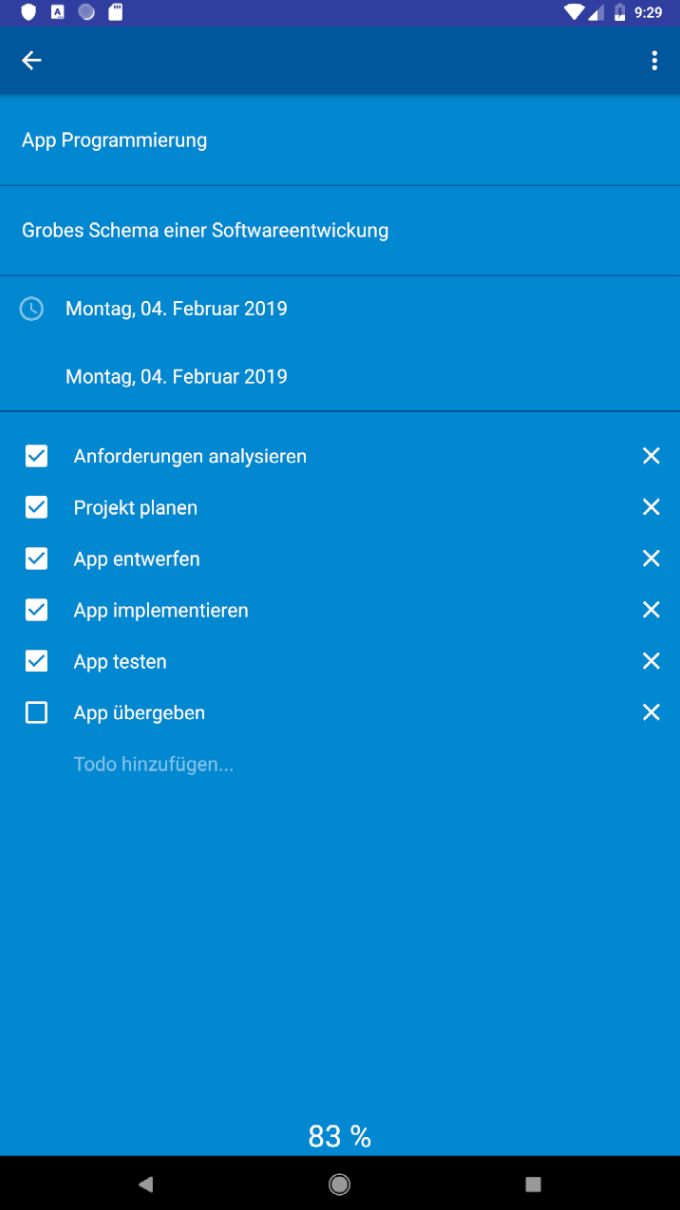
\includegraphics[height=20cm]{img/Todo_portrait}\\ % Pfad
\source{Screenshot aus der Benutzeroberfläche} % Quelle
\end{minipage}
\end{figure}

Nachdem auf eines der Eingabefelder für Daten getippt wurde, initialisiert die Activity einen Datepicker und zeigt dem Benutzer ein gewohntes Auswahlmenü für ein gewünschtes Datum an. Dies hat den Vorteil, dass der Benutzer durch Erfahrungen in anderen Apps schnell und einfach mit der Datumeingabe zurechtfindet. Wie im Screenshot zu sehen ist, kann der Benutzer mit „Abbrechen“ die Datumsauswahl abbrechen, sodass das Eingabefenster geschlossen wird. Mit dem „Ok“-Button hat der Benutzer alternativ die Möglichkeit, seine Eingabe zu übernehmen. Hierbei liest die Activity das eingegeben Datum aus und stellt es formatiert dar. Es wird außerdem indem Todo-Objekt zwischengespeichert.

\begin{figure}[H]
\centering
\begin{minipage}[t]{1\textwidth} % Breite, z.B. 1\textwidth		
\caption{Datumeingabe} % Überschrift
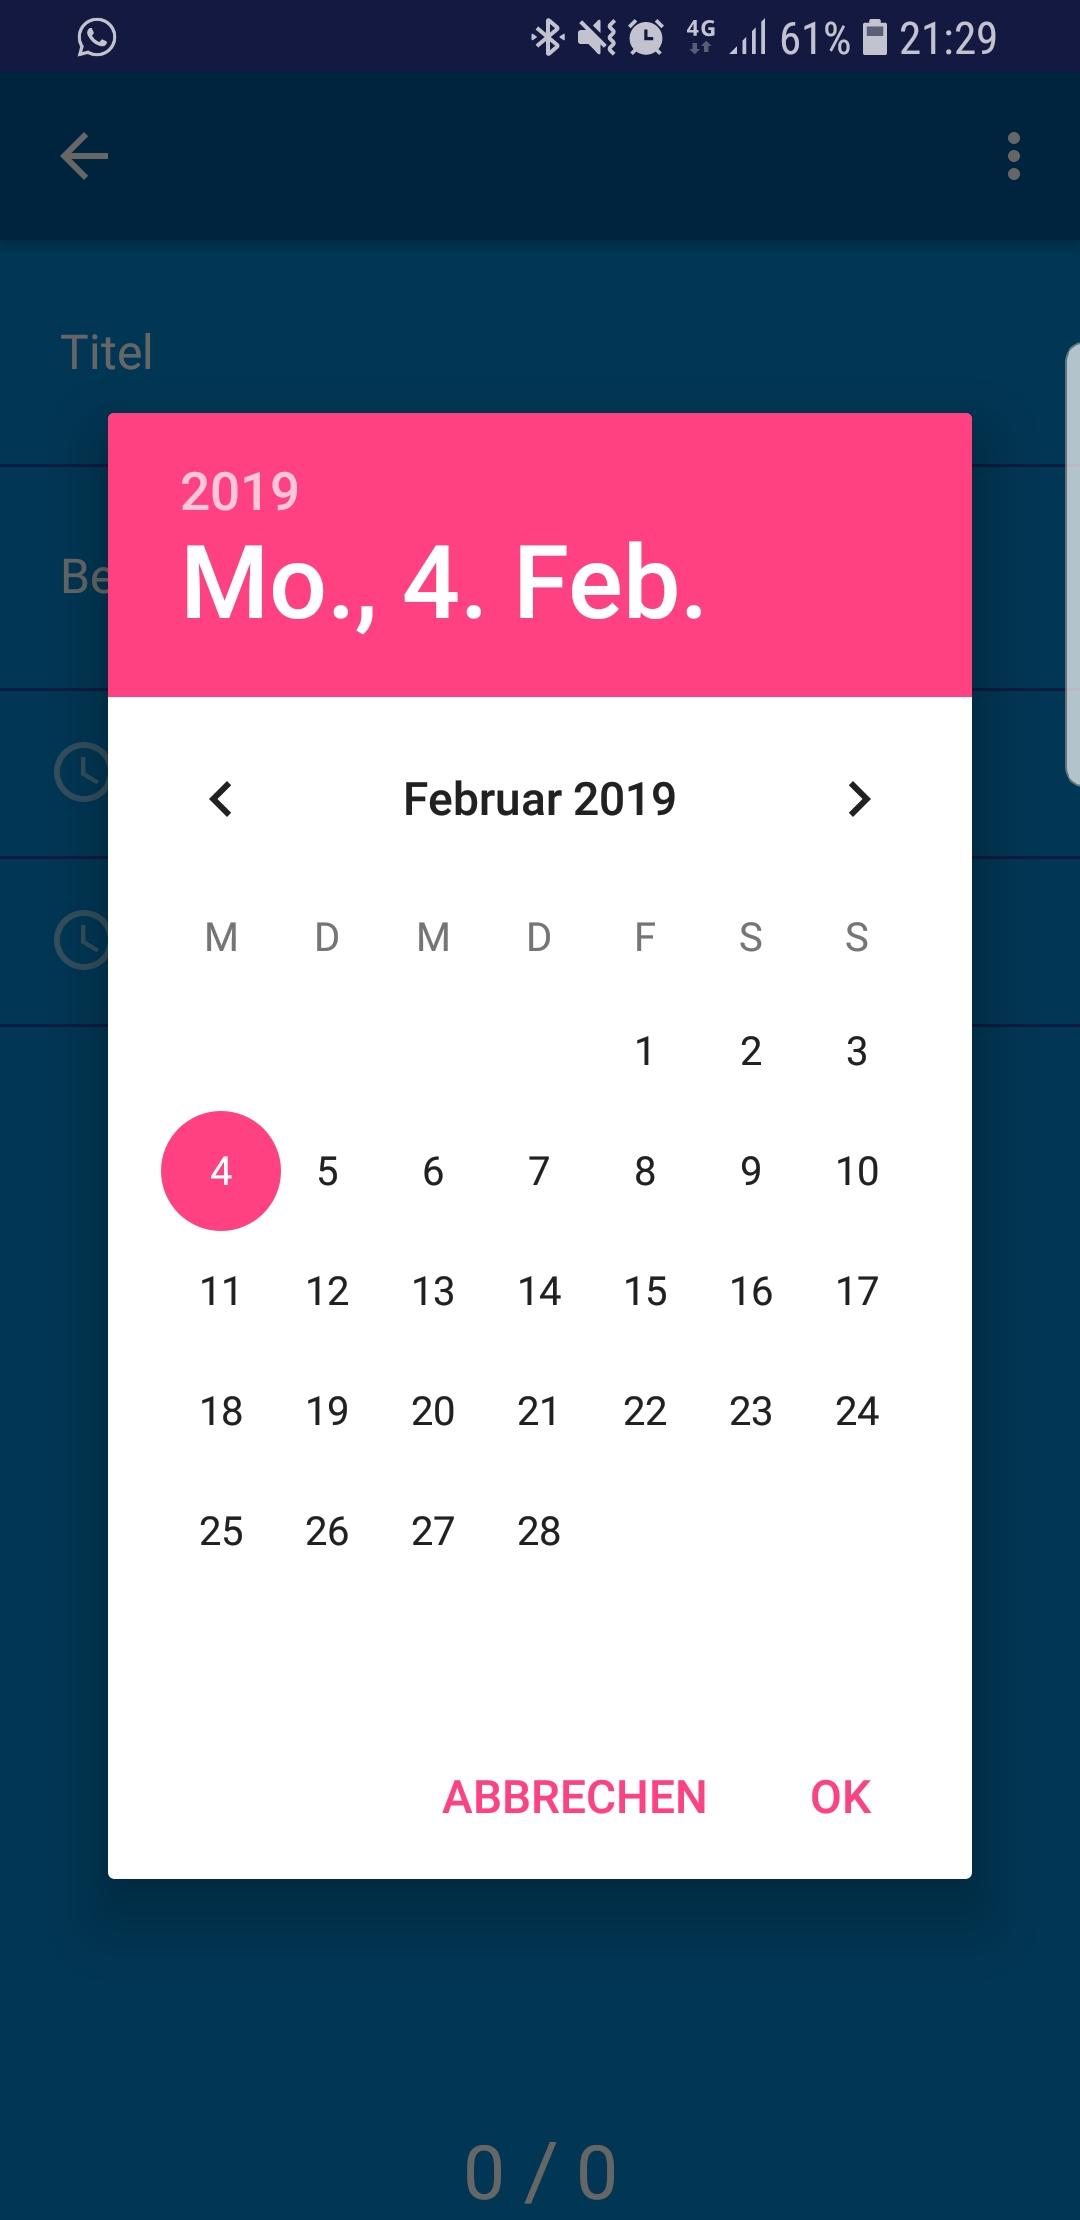
\includegraphics[height=20cm]{img/Todo_Datepicker}\\ % Pfad
\source{Screenshot aus der Benutzeroberfläche} % Quelle
\end{minipage}
\end{figure}

%Florian
\paragraph{Use Case (Florian Rath)}
Die Todo-Activity kann man über zwei Wege erreichen. Beide Wege erfolgen aus der Übersichts-Activity.

Der User kann entweder eine neue Todo erstellen, sodass in der Todo-Activity eine nicht vorhandene Todo-ID übergeben wird, oder er kann auf eine bereits vorhandene Todo tippen. Die ID dieser Todo wird dann aus der Datenbank geladen und in der Activity dargestellt. Die Todo-Activity deckt die Funktionalitäten des Todo-TEN‘s ab.

%Sertan
\paragraph{Datenstrukturen und -typen (Sertan Cetin)}
Um die gewünschten Anforderungen zu erfüllen und dabei sowohl eine hohe Wartbarkeit als auch Modularität zu gewährleisten, wurden innerhalb der Todo-Activity mehrere Klassen implementiert. Nachfolgend werden diese Klassen vorgestellt.

Wenn die Todo-Activity aus der Overview-Activity gestartet wird, wird eine Instanz der Klasse Init, die die Schnittstelle AppCompatActivity implementiert, erstellt. In dieser Klasse werden weitere Klassen, die im Rahmen des Projektes angelegt wurden, erstellt. Bei diesen Klassen handelt es sich um Gui, TodoApplicationLogic und Data. Auf diese wird im Nachfolgenden näher eingegangen.

Die Gui-Klasse ist die Schnittstelle zum Layout. Hier werden alle Layout-Elemente in Variablen bzw. typgleichen Objekten gespeichert. So wird z.B. das Eingabefeld für den Titel in einer Variablen vom Datentyp EditText gespeichert. Indem jedes Element aus dem Layout in einer Variablen hinterlegt wird, erhält man die Möglichkeit diese vom Java-Code aus auszulesen bzw. zu manipulieren. Diese Klasse besitzt einen Konstruktor, in welchem die eigentliche Erstellung der genannten Objekte geschieht. Über Getter- und Setter-Methoden stellt die Gui-Klasse den anderen Klassen die Schnittstelle zum Layout zur Verfügung.

Die Data-Klasse speichert das Todo und stellt die Schnittstelle zwischen der Datenbank und der Applikationslogik dar. Sie ist somit für das Speichern, Löschen und Ändern verantwortlich. Im Konstruktor dieser Klasse wird außerdem das Todo-Objekt initialisiert. Beim Initialisierungsvorgang der Data-Klasse wird eine ID übergeben. Ist diese ID nicht vorhanden, wird legt sie ein neues Todo in der Datenbank an. Andernfalls wird das Todo geladen.

In der TodoApplicationLogic-Klasse findet die gesamte Geschäftslogik statt. Sie verbindet im Wesentlich die Data mit der Gui. Sie ist unteranderem für die Interaktion zuständig.

\paragraph{Dokumentation des Quelltextes der Activity}
In diesem Kapitel wird der Quelltext der \textit{Todo-Activity}\ vorgestellt und erläutert. Dabei wird Klasse für Klasse, Methode für Methode vorgegangen.

\subparagraph{Methoden der Init-Klasse (Sertan Soner Cetin)}

Die Init Klasse verfügt insgesamt über 10 Methoden. Da die Klasse die Schnittstelle AppCompatActivity implementiert, sind die Methoden onCreate, onCreateOptionsMenu, onSaveInstanceState, onActivityResult, onBackPress und onConfigurationChanged vorhanden. Daneben sind noch Methoden wie initData, initGUI und initApplicationLogic vorhanden.

\textit{Private void initApplication()}

Diese Methode initialisiert das Objekt des Typs TodoApplicationLogic. Diese ApplicationLogic erhält die GUI- und Data-Objekte

\textit{Private void initData(String todoId)}

Diese Methode initialisiert das Data-Objekt des Datentyps Data. Das Objekt erhält eine Instanz zur Activity und eine Todo-ID vom Typ String, welche dieser Methode ebenfalls übergeben wird.

\textit{Private void initGui()}

Diese Methode initialisiert das Gui-Objekt. Dieses Objekt erhält eine Instanz zu der Activity.

\textit{Public void onCreate(Bundle savedInstanceState)}

Diese Methode wird beim Erstellvorgang der Init-Klasse aufgerufen. Sie ruft die zuvor beschriebenen Methoden auf. Der Parameter savedInstanceState wird der Oberklasse übergeben.

\subparagraph{Methoden der Gui-Klasse (Sertan Soner Cetin)}

Die Gui-Klasse verfügt über einen Konstruktor, der im vorangegangenen Kapitel beschrieben wurde. Außerdem verfügt sie über diverse Getter- und Setter-Methoden. Es werden einige exemplarisch dargestellt.

\textit{Public void setFocusableInTouchmode(boolean value)}

Diese Methode stellt den TouchModus des Layouts aus. Über den Parameter value kann angegeben werden, ob sich die Tastatur beim Start des Layouts aufklappen soll oder nicht. (true für nicht ausklappen, false für ausklappen)

\textit{Public EditText getmTitle()}

	Diese Getter-Methode liefert das Objekt mTitle des Datentyps EditText zurück.

\textit{Public void setmTitle(string pTitle)}

Diese Setter-Methode schreibt in das Textfeld des Todo-Layouts den übergebenen Parameter mit dem Namen pTitle des Datentyps String.

\textit{Public EditText getmText()}

Diese Getter-Methode liefert das Objekt mText des Datentyps EditText zurück. Das Objekt entspricht dem Layout-Element für die Beschreibung des Todos.

\textit{Public void setColor(int color, int darkColor)}

An diese Methode werden zwei Farbwerte als Integer übergeben. Der erste Farbwert entspricht einem helleren Farbton, z.B. Hellblau. Der zweite wäre ein dunklerer Blauton, z.B. Dunkelblau. Das Layout bekommt die helle Farbe als Hintergrundfarbe, während die Toolbar oder Trennlinien zwischen den einzelnen Elementen die dunklere Farbe erhalten.

\subparagraph{Methoden der Data-Klasse (Sertan Soner Cetin)}

Diese Klasse verfügt über einen Konstruktor und über Getter- und Setter-Methoden. Durch die Schnittstelle zur Datenbank sind noch Methoden für das Löschen und Ändern der Todo in der Datenbank vorhanden.

\textit{Public void deleteTodo()}

	Löscht die Todo aus der Datenbank anhand seiner ID.

\textit{Public void updateTodo()}

	Ändert die Todo in der Datenbank und aktualisiert somit alle Eigenschaften.

\textit{Public void setTitle(string title)}

Ändert den Titel der Todo. Der Parameter title des Datentyps String ist der neue Titel.

\textit{Public boolean getmIsNew()}

Gibt an, ob die Todo neuerstellt wurde oder beim Start der Activity bereits vorhanden war. Dieser Wert wird außerhalb benötigt, um festzulegen, ob sich die Tastatur beim Activity-Start aufklappen soll oder nicht.

\subparagraph{Methoden der TodoApplicationLogic (Florian Rath)}

Die TodoApplicationLogic stellt die größte Klasse innerhalb der Todo-Activity dar. Dies liegt unter anderem daran, dass die meisten Verantwortlichkeiten hier liegen. Sie ist Dreh und Angelpunkt der gesamten Infrastruktur, da sie die Data bzw. Datenbank mit der Gui bzw. dem Layout verbindet und alles steuert.

\textit{Private void initGui()}

Diese Methode stellt die Gui ein und ruft eine andere Methode namens dataToGui auf.

\textit{Private void dataToGui()}

Diese Methode schreibt die Todo-Eigenschaften auf die einzelnen Layout-Elemente. So wird z.B. der Todo-Titel in das Eingabefeld für den Titel geschrieben oder die Farbe des Todos als Hintergrundfarbe festgelegt.

\textit{Private void initListener()}

Da innerhalb der Applikationslogik die Listener für die einzelnen Events z.B. ClickEvent oder TouchEvent verwaltet werden, wurde diese Methode angelegt, um alle Listener an einer zentralen Stelle zu initialisieren. Hier werden der ClickListener, TouchListener und CheckedChangeListener initialisiert und bei den einzelnen Layout-Elementen registriert.

\textit{Public void receiveDate(Date date)}

Diese Methode wurde für den Datepicker benötigt. Sie empfängt quasi das Datum aus dem Eingabefeld. Der Parameter date wird dann an das Eingabefeld übergeben.

\textit{Public String formatDate(Date date)}

Diese Methode liefert einen String zurück. Der Parameter date wird in eine leserliche Formatierung gebracht. Die Formatierung des Datums ist z.B. „Dienstag, 13. Januar 2019“.

\textit{Public void showDatePickerDialog(View v)}

Diese Methode initialisiert das DatePickerFragment. Dazu wird der Parameter v benötigt, um die beiden Start- und Enddatum-Felder unterscheiden zu können, da beide denselben DatePicker verwenden.

\textit{Public void returnToOverview()}

Diese Methode leitet den Benutzer wieder zur Overview-Activity zurück. Bei diesem Vorgang wird außerdem die UpdateTodo-Methode aufgerufen, die weiter unten beschrieben ist.

\textit{Public void onMenuItemClick(MenuItem item)}

Bei dieser Methode handelt es sich um einen Event-Handler. Diese wird ausgeführt, wenn ein Menü-Item angeklickt wird. Da nur ein Menüpunkt vorhanden ist, ist es eindeutig. An dieser Stelle wird die externe Methode des Data-Objekts deleteTodo aufgerufen. Außerdem wird die zuvor beschriebene returnToOverview-Methode aufgerufen.

\textit{Public void createList()}

Diese Methode erzeugt eine Liste bzw. initialisiert den TaskAdapter. Der TaskAdapter wird benötigt, um aus einer Liste von Tasks in eine ListView-Elementliste zu verwandeln. Dieser Adapter wird dem GUI-Element ListView zugewiesen.

\textit{Private void addTask()}

Diese Methode fügt Tasks-Liste, welche in der GUI angezeigt wird, ein Element hinzu.

\textit{Public void updateProgress()}

Die updateProgress-Methode holt sich aus dem Todo-Objekt den Anteil der erledigten Aufgaben. Dieser Wert wird in eine Prozentzahl umgewandelt. Der Prozentwert wird dem entsprechenden Layout-Element zugewiesen.

\textit{Private void onEditTextClicked()}

Bei dieser Methode handelt es sich um einen Event-Handler. Dieser wird ausgeführt, wenn auf ein EditText-Feld getippt wurde. Dabei wird ein neues EditText-Feld erzeugt, um eine weitere Aufgabe eingeben zu können.

\textit{Public void onActivityReturned(int requestCode, int resultCode, Intent data)}

	Diese Methode deckt den Fall ab, falls in die Activity zurückgekehrt wird.

\textit{Private void onDelteButtonClicked(int id)}
Es wird dieser Methode eine ID übergeben. Diese ID entspricht der Aufgabe, bei der der Lösch-Button geklickt wurde. Anhand dieser ID wird der Task aus der Liste entfernt.

\textit{Private void onTextChanged(String s, View mView)}

Bei dieser Methode handelt es sich um einen Text-Changed Event-Handler. Der Parameter s steht für den Text und mView für das Element. Handelt es sich um den Titel, wird die setTitle-Methode des Data-Objekts aufgerufen. Handelt es sich um die Beschreibung, wird die setText-Methode desselbigen Objekts aufgerufen.

\textit{Public void onOkButtonClicked()}

Wenn der OK-Buttons des Datumeingabefelds geklickt wird, wird die Methode UpdateTodo aufgerufen.

\textit{Public void onBackPressed()}

Wird der Zurück-Button aus der Toolbar gedrückt, wird die UpdateTodo-Methode aufgerufen. So wird beim Verlassen der Activity die Todo in der Datenbank gespeichert.

\textit{Private void addInputTaskField()}

Fügt der Task-Liste ein weiteres Element hinzu. Außerdem wird der TaskAdapter benachrichtigt, um die GUI zu aktualisieren. Hierdurch wird auch der prozentuale Anteil der erledigten Aufgaben beeinflusst, weshalb die Methode updateProgress aufgerufen wird.

\textit{Public ArrayList<Task> getmTasks()}

Liefert die ArrayList mit Task-Objekten zurück.

\textit{Private int getTasksItemCount()}

Liefert eine Zahl zurück, die angibt, wie viele Elemente in der Task-Liste gespeichert sind.

\textit{Public ClickListener getClickListener()}

Gibt das ClickListener-Objekt zurück.

\textit{Public TouchListener getTouchListener()}

	Gibt das TouchListener-Objekt zurück.

\textit{Public CheckedChangeListener getmCheckedChangeListener()}

	Gibt das CheckedChangeListener-Objekt zurück.

\textit{Public void UpdateTodo()}

Diese Methode speichert zuerst das Todo-Objekt aus der Data-Klasse in einer lokalen Todo-Methodenvariable. Von diesem werden der Titel und Beschreibung gesetzt. Das Start- und Enddatum werden ebenfalls aktualisiert. Am Ende der Methode wird das Todo in der Datenbank gespeichert bzw. aktualisiert.

\textit{Public void onConfigurationChanged(Gui pGui)}

Bei dieser Methode handelt es sich um einen Event-Handler. Diese initialisiert die Gui und Listener erneut. Dazu werden die beschriebenen Methoden initGui und initListener aufgerufen.


\newpage
\subsubsection{Event Activity}
\fancyhead[L]{Event Activity}
%Robin
Dieses Kapitel beschreibt die Funktionsweise der Event-Ansicht innerhalb des TEN-Managers. Diese wird aufgerufen, wenn ein Event aus der Übersichtsseite angeklickt wird oder ein neues Event erstellt wird.

\paragraph{Aufgaben und Funktionen (Robin Menzel)}

Die \textit{Event Activity} hat die Funktion eine Übersicht über ein Event zu geben, Bearbeitungen zu dem Event zu verarbeiten, oder ein neues Event zu erstellen und speichern. Möchte ein User eine neues Event erstellen, ist die Event-Activity bis auf das aktuelle Datum leer. In den Textfeldern stehen halbtransparente Hinweise, wie "Titel eingeben", die dem User Hinweise über den Inhalt geben. Wenn die Activity ein bereits vorhandenes Event anzeigt, kann durch ein Klick auf die jeweilige Konfiguration, eine Änderung durchgeführt werden.

Ganz oben ist eine Toolbar zu finden, welche zum einen eine Navigation zurück zur Übersichtsseite bietet und zum anderen ein Options/Drei-Punkt Menü beinhaltet. Durch einen Klick auf das 3-Punkt Menu der \textit{Event Activity}  kann das Event in Form von Text per E-Mail oder Chat-Applikation geteilt werden. Auch ein Export in eine andere Kalender-Applikation wird hier unterstützt. Die letzte Option bietet das Löschen des Events an.

Da ein Event immer ein Datum und eine Zeit hat, kann auch dieses in der Activity ausgewählt werden. Über einen Klick auf das Datum oder die Uhrzeit, öffnet sich ein Dialog Picker, über den sich die Uhrzeit oder das Datum auswählen lässt.

Bestimmte Events wie Geburtstage wiederholen sich in bestimmten Intervallen. Auch diese Events lassen sich in der Activity abbilden, in dem unter der Zeit auf (initialer Wert) Einmalig geklickt wird. Hier steht dem User die Option Einmalig, Täglich, Wöchentlich und Jährlich zur Verfügung. Angezeigt wird immer der Termin, der am nächsten liegt.

Sobald ein User mehr als einen Buchstaben in die Adresszeile des Events eingibt, leuchtet das Navigationsicon auf. Ein klick auf dieses öffnet sich Google Maps und versucht den eingegeben Ort zu finden.

Als letzte Option lassen sich Erinnerungen zu diesem Event einstellen. Dazu hat der User eine Wahl zwischen 1 Stunde vorher, 6 Stunden vorher, 1 Tag vorher und 1 Woche vorher. Es lassen sich kein, ein, mehrere, oder alle Erinnerungen auswählen. Liegt der Zeitpunkt der Erinnerung in der Zukunft, so wird zu diesem Zeitpunkt eine Push-Benachrichtigung auf dem Gerät erscheinen, welche den Titel und die Uhrzeit des Events enthält.

\paragraph{Layout (Robin Menzel)}

Das Layout der Activity setzt sich aus verschieden Komponenten zusammen:
\begin{itemize}
\item \textit{activity\_event.xml}
\item \textit{toolbar\_ten.xml}
\end{itemize}
Bei \textit{activity\_event.xml} handelt es sich um ein Drawer Layout. Es beinhaltet die Toolbar \textit{toolbar\_ten.xml}. Die Inhalte sind in einem Scroll View zusammengefasst.

Die Toolbar \textit{toolbar\_ten.xml} ist für alle TENs identisch und beinhaltet ein Drei-Punkt-Menu mit den Menüpunkten aus \textit{event\_menu.xml}
\begin{itemize}
\item Event teilen
\item Event in den Kalender
\item Event löschen
\end{itemize}

\begin{figure}[H]
\centering
\begin{minipage}[t]{1\textwidth} % Breite, z.B. 1\textwidth		
\caption{Screenshot - Event Activity} % Überschrift
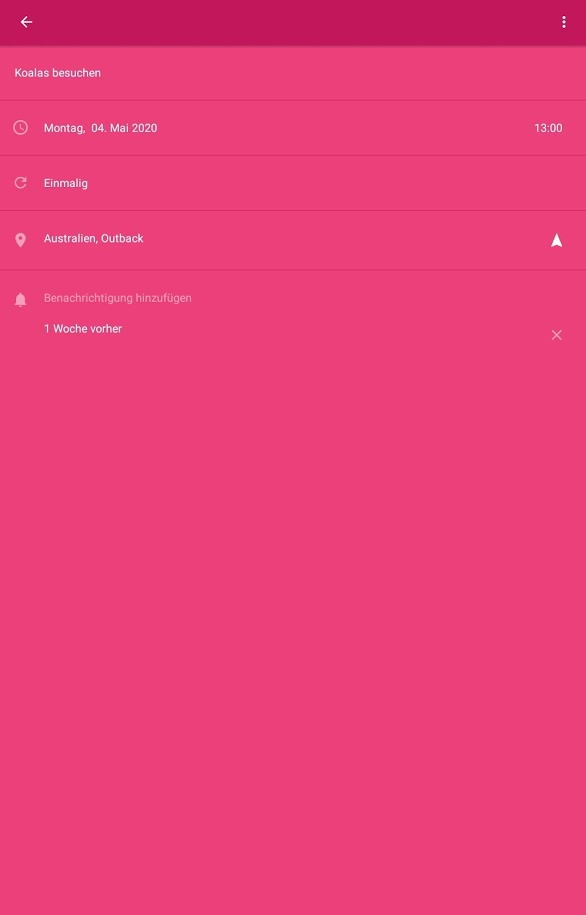
\includegraphics[width=13 cm]{img/Screenshot_EventActivity.jpg}\\ % Pfad
\source{Screenshot aus der Benutzeroberfläche} % Quelle
\end{minipage}
\end{figure}

\begin{figure}[H]
\centering
\begin{minipage}[t]{1\textwidth} % Breite, z.B. 1\textwidth		
\caption{Screenshot - Event Activity Erinnerung} % Überschrift
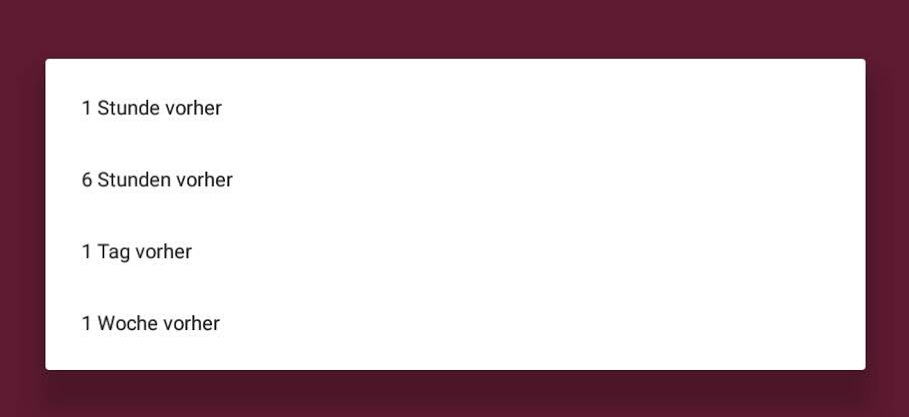
\includegraphics[width=13 cm]{img/Screenshot_EventActivityReminder.jpg}\\ % Pfad
\source{Screenshot aus der Benutzeroberfläche} % Quelle
\end{minipage}
\end{figure}

\begin{figure}[H]
\centering
\begin{minipage}[t]{1\textwidth} % Breite, z.B. 1\textwidth		
\caption{Screenshot - Event Activity Wiederholung} % Überschrift
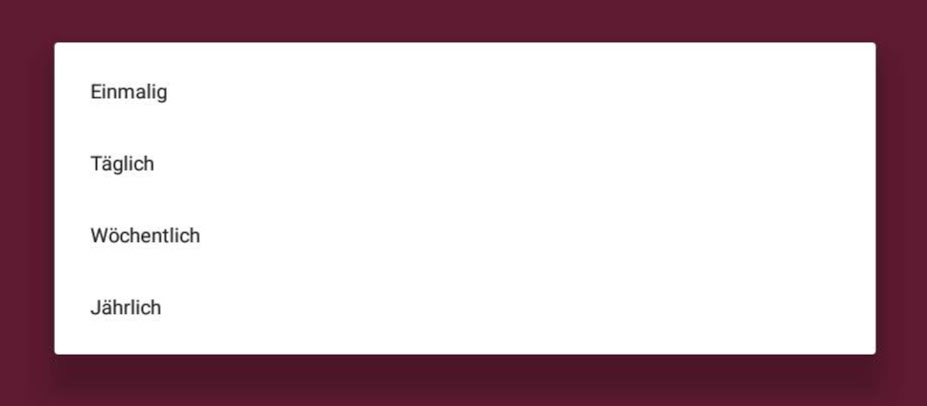
\includegraphics[width=13 cm]{img/Screenshot_EventActivityRecurringType.jpg}\\ % Pfad
\source{Screenshot aus der Benutzeroberfläche} % Quelle
\end{minipage}
\end{figure}

\begin{figure}[H]
\centering
\begin{minipage}[t]{1\textwidth} % Breite, z.B. 1\textwidth		
\caption{Screenshot - Event Activity Toolbar} % Überschrift
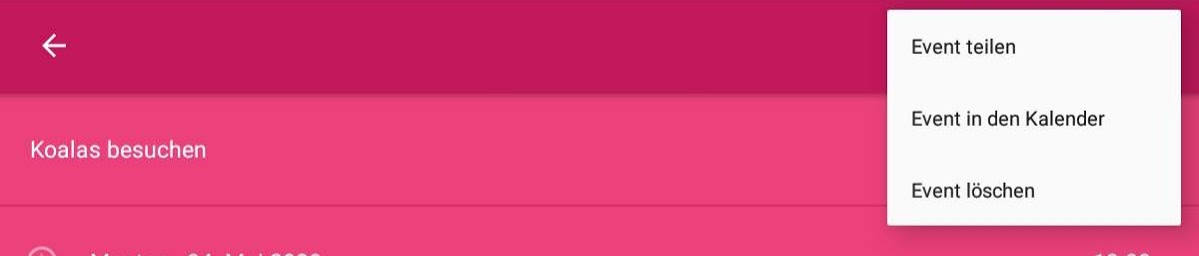
\includegraphics[width=13 cm]{img/Screenshot_EventActivityToolbar.jpg}\\ % Pfad
\source{Screenshot aus der Benutzeroberfläche} % Quelle
\end{minipage}
\end{figure}

\paragraph{Use-Case (Robin Menzel)}
Diese Activity dient dem User hauptsächlich zum Anlegen, Bearbeiten, Ansehen und Löschen von einem Event. Außerdem ist die Activity verantwortlich für alle Reminder, die als Push-Benachrichtigung erscheinen und an das jeweilige Event erinnern. In der Activity ist es des Weiteren möglich, über einen Button Google Maps inklusive der Adresse des Events zu öffnen und so zu dem Event zu Navigieren. Außerdem ist es möglich das Event in Form von Text zu teilen (z.B. per E-Mail oder Textnachricht) oder in eine Kalender Applikation zu übertragen.

\begin{figure}[H]
	\centering
	\caption{Use-Case - Event Activity}
	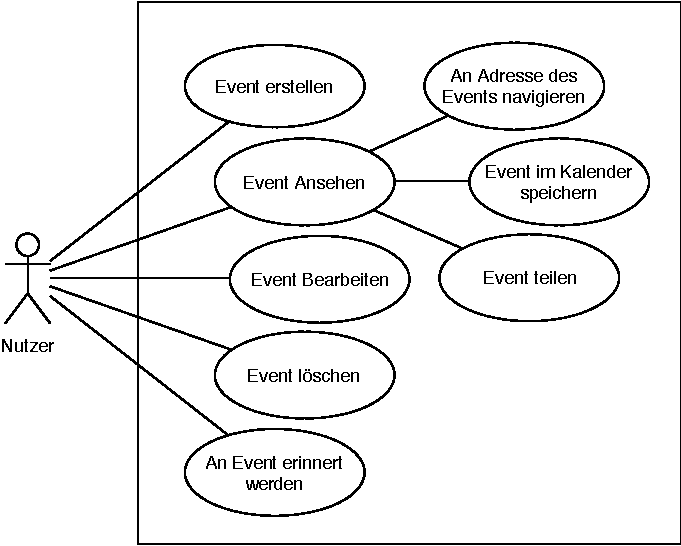
\includegraphics[width=12cm]{img/EventActivityUseCase.pdf}
	\label{img:EventActivityUseCase}
\end{figure}

\paragraph{Datenstruktur und -typen (Robin Menzel)}
Die \textit{Event Activity} wird aus der \textit{MainActivity} mittels eines Intents gestartet, welcher falls das Event bereits besteht und kein neues Event angelegt werden soll, die jeweilige ID des Events übergibt, um darüber auf die Datenbank zuzugreifen. Die Klasse EventActivit ist aus der Klasse AppCompatActivity abgeleitet und überschreibt die für die Funktionen relevanten Methoden diese Klasse und initialisiert die im Nachfolgenden angesprochenen Verwaltungsklassen EventData, EventGui und EventApplicationLogic.

Die Event-Activity selbst ist in mehrere Pakete aufgeteilt um innerhalb der insgesamt 14 Klassen für eine übersichtliche Struktur zu sorgen und die einzelnen Klassen ihren übergeordneten Funktionen zuzuordnen. Die Funktionen der einzelnen Klassen und die Klasseninteraktion sind in der Dokumentation des Quelltextes am Ende dieses Kapitels dargestellt.

\subparagraph{Logic Paket}
Das Paket welches die Logik der \textit{Event Activity} beinhaltet, beinhalten alle Listener und Watcher Klassen und die \textit{EventApplicationLogic}. Damit ist sie die zentrale Logik-Klasse der Activity. Von hier aus werden die andren Klassen, welche spezifische Aufgaben übernehmen, initialisiert und angesprochen. Zu den anderen Klassen gehören die Klassen zur Erneuerung der GUI, des automatischen Speichern von Änderungen und den Klassen zur Verwaltung von Erinnerungen.

\subparagraph{Data-Paket}
Das Data-Paket beinhaltet alle Klassen welche für die Datenhaltung zuständig sind. Zentrale Klasse ist hier die \textit{EventData-Klasse} welche für das Laden, aber auch das Speichern von Änderungen bzw. neuen Events zuständig ist. Zudem beinhaltet das Data-Paket eine Reminder Klassse, welche dafür sorgt, dass Reminder zum einen als Zeitpunkt der Erinnerung, aber auch in Text-Form (``1 Stunde vorher'') genutzt werden kann. \\
Die \textit{Event Activity} interagiert neben der \textit{Overview Activity} auch mit anderen Apps. Entweder durch die ShareAction oder durch die Google Maps Intents.

\subparagraph{Gui-Paket}
Innerhalb des Gui-Paketes subd alle Klassen einsortiert, welche die für die Darstellung der GUI verantwortlich sind. Die EventGui Klasse repräsentiert die Struktur des Layouts und damit alle einzelnen Komponenten, um diese korrekt zu initialisieren und auf einzelne Views zugreifen zu können. Außerdem enthält das Paket die Dialog Picker TimePicker und DatePicker, die für die Auswahl eines Datums bzw. einer Uhrzeit zuständig sind. Zu guter letzt hilft die RecurringTypeHelper dabei die Wiederholungen als Zahlen, aber auch in Textform (``Einmalig'') abbilden zu können.

\paragraph{Dokumentation des Quelltextes der Activity (Robin Menzel)}
Im Nachfolgenden sind die einzelnen Klassen der \textit{Event Activity} mit den jeweiligen wichtigsten Funktionen kurz beschrieben.
\subparagraph{EventActivity}
Diese Klasse ist der zentrale Einstiegspunkt der Note-Activity und ist aus der AppCompatActivity-Klasse abgeleitet. Hier werden eineige Methoden dieser Klasse überschrieben und an die neuen Anforderungen angepasst.

\textit{onCreate}:\\
Die Activity wird durch einen Intent von der \textit{Overview Activity} gestartet, welchem die ID für ein Event mitgegeben wurde. Diese ID wird ausgelesen und anhand dieser die Event-Data Klasse initialisiert. Zusätzlich wird die EventGui und die EventApplicationLogic Klasse initialisiert.

\textit{onBackPressed}:\\
In dieser Methode wird das normale vorgehen ersetzt durch die Funktion returnToOverview der EventApplicationLogic um wieder in die Overview-Klasse zurückzukehren.

\textit{onCreateOptionsMenu}:\\
In dieser Methode wird das Menü mit dem Event Menü gefüllt.\\

\subparagraph{LOGIC}
\subparagraph*{EventApplicationLogic}
Diese Klasse ist die zentrale Logik der Activity.\\
\\
\textit{updateGui}\\
Diese Methode setzt alle Werte aus dem Event-Objekt aus der EventData Klasse in die aktuelle Gui ein.\\
\\
\textit{returnToOverview}\\
Mit Hilfe dieser Methode wird die Activity verlassen und kehrt zurück zur Overview Activty.\\
\\
\textit{setAlarm}\\
Wenn ein Reminder erstellt wird, wird hier der Zeitpunkt zum AlarmManager hinzugefügt (solange der Zeitpunkt in der Zukunft liegt).\\
\\
\textit{updateReminder}\\
Wenn sich die Zeit verändert, müssen auch die Zeitpunkte der Reminder angepasst werden. Dies geschieht in dieser Methode.\\
\\
\textit{onNewReminderClicked}\\
Diese Methode kümmert sich um das Erstellen eines neuen Reminders, solange noch nicht alle vier möglichen Reminder hinzugefügt wurden.\\
\\
\textit{onTextChanged}\\
Sobald der Textwatcher ausgelöst wird, wird diese Funktion aufgerufen um das Event Objekt dynamisch zu speichern.\\
\\
\textit{onCloseReminderClicked}\\
Diese Methode kümmert sich um das Löschen einer Reminders. Dazu gehört auch, diesen aus dem Alarm Manager zu entfernen.\\
\\
\textit{onMenuItemClicked}\\
Diese Methode wird aufgerufen, sobald auf einen der drei Menüpunkte geklicked wurde.\\
\\
\textit{onNavicationIconClicked}\\
Wurde auf das Icon neben der Adresse geklickt, so erstellt diese Funktion einen Google Maps Intent, der die Adresse in Google Maps öffnet.\\
\\
\textit{onRecurrinTypeClicked}\\
Diese Funktion öffnet einen AlertDialog in welchem man den Wiederholungstypen auswählen kann.

\subparagraph{listener Klassen}
Die listener Klassen in dem LOGIC Paket erben alle von View.onClickListener, text.TextWatcher und Toolbar.onClickListener. In ihnen wird differenziert welches Element den Listener ausgelöst hat und führt dementsprechend eine Methode aus.


\subparagraph{DATA}
\subparagraph*{EventData}
In dieser Klasse findet die komplette Datenhaltung statt.\\
\\
\textit{updateEvent}\\
In dieser Methode wird des Services ``Update'' der Datenbank genutzt um ein Event-Objekt zu speichern.\\
\\
\textit{deleteEvent}\\
In dieser Methode wird des Service ``Delete'' der Datenbank genutzt um ein Event-Objekt zu löschen.\\
\\
\textit{shareEvent}\\
Diese Methode wird Aufgerufen falls der User im ein Event teilen möchte. Von hier aus wird die shareEvent-Methode im ShareModule aufgerufen.\\
\\
\textit{getFormateDate}\\
Diese Methode gibt das Datum des Events in sprach-formattierung zurück, wie z.B. 25. Januar 2019.\\
\\
\textit{exportToCalendar}\\
Diese Methode erstellt aus dem Event ein Intent, welches von allen gängigen Kalender Applikationen untersützt und geöffnet werden kann.\\
\subparagraph{Reminder}
Diese Klasse hilft beim Umgang mit Remindern. So müssen z.B. Reminder neu berechnet werden, wenn sich die Zeit des Events verändert hat.\\
\\
\textit{getLabelFromReminder}\\
Diese Methode gerrechnet aus der Differenz zwischen dem Zeitpunkt der Erinnerung und dem Zeitpunkt des Events die Beschriftung (z.B. ``1 Stunde vorher'').\\
\\
\textit{getReminderFromLabel}\\
Diese Methode errechnet aus der Beschrifftung den richtigen Zeitpunkt einer Erinnerung.

\subparagraph{GUI}
\subparagraph*{EventGui}
Diese klassse beinhaltet alle Benutzeroberflächenattribute, auf welche so zugegriffen werden kann.\\
\\
\textit{setColor}\\
Die bunte Farbgestalltung ist ein Kernelement unseres Designs. Daher enthält jedes TEN-Objekt auch feste Farbattribute, welche beim Aufbau der Gui dargestellt werden müssen. Diese Methode weißt aus den Farbwerten des Event-Objektes, den Gui Elementen ihre spezifische Farbe zu.\\
\\
\textit{setReminder}\\
Diese Klasse stellt die Reminder, die im Event-Objekt nur als Zeitpunkte dargestellt sind, auf der Oberfläche da. Dafür interagiert diese mit der Reminder Klasse und passt auch das Auswahl-Menü für weitere Reminder an.

\subparagraph{DatePicker und TimePicker}
Diese Klassen sind fast identisch. Sie erben von der Klasse DialogFragment und überschreiben notwendige Methoden.\\
\\
\textit{onCreateDialog}\\
In dieser Methode wird ein Calendar Objekt erstellt um in ihm später die Ausgewählten Zeiten zu speichern. Falls bereits eine Zeit existiert, wird diese übernommen. Anschließend wird ein DatePickerDialog erstellt.\\
\\
\textit{onDateSet} oder \textit{onTimeSet}\\
Falls eine Zeit ausgewählt wurde, ruft diese Methode, die entsprechenden Methoden in der EventApplicationLogic auf und übergibt die ausgewählten Zeite.\\
\\
\textit{setTime}\\
Da über einen Konstruktor eine vorhandene Zeit eines Events noch nicht übergeben werden kann, muss der Date/Time-Picker zuerst erstellt werden und anschließend kann über diese Methode die bereits vorhandene Zeit eingestellt werden.

\subparagraph{RecurringTypeHelper}
Diese Funktion stellt eine Verbindung zwischen dem Enum Objekt ReccuringType und den Beschriftungen der Wiederholungen her.

\newpage
\subsubsection{Note Activity}
\fancyhead[L]{Note Activity}
Im Folgenden wird die Funktionsweise der Notiz-Ansicht innerhalb des TEN-Managers be-schrieben, welche bei Erstellung einer neuen Notiz beziehungsweise dem Öffnen einer bereits bestehenden Notiz aufgerufen wird. Da eine Notiz auch Stichworte enthalten kann, besteht für die Bearbeitung dieser zusätzlich eine weitere Activity.

\paragraph{Aufgabe und Funktion (Joscha Nassenstein)}
Die Notiz-Activity soll, wie der Name es schon besagt, dem Nutzer ermöglichen, eigene Notizen anzulegen. Zu den Inhalten einer Notiz zählen dabei ein Titel, eine Beschreibung sowie eine Menge von Bildern und Stichworten. Die Bilder können aus der Notiz heraus aufgenommen beziehungsweise aus der Galerie in die Notiz importiert werden. Die Stichworte können in einer weiteren Ansicht anhand einer dynamischen Liste hinzugefügt, bearbeitet und entfernt werden. Desweiteren ist es möglich, ein Bild in Großansicht aufzurufen und anhand von Wischgesten zwischen den Bildern zu Wechseln. Allgemein wurde versucht, eine intuitive Bedienung der Notizansicht zu ermöglichen.

\paragraph{Layout, Screenshots (Joscha Nassenstein)}
In der Planung der Notiz-Activity wurde bei der Implementierung der Darstellung der Bilder etwas von der zuvor erstellten MockUp-Ansicht abgewichen, um eine einheitliche Darstellung, aber bei Bildern mit verschiedenen Seitenverhältnissen, zu ermöglichen und diese ohne einen schwarzen Rand darstellen zu können. Zusätzlich sollte der Fokus auf die Notiz selbst gelegt werden, weshalb die Bilder am äußeren Bildschirmrand und etwas kleiner platziert wurden.

Zunächst wurden die XML-Layouts für die die beiden Ansichten erstellt. Dabei wurden für die beiden Texteingabefelder jeweils ein EditText-Element verwendet. Zusätzlich wurde für die Stichwörter ein TextView aufgenommen, welches bei einer Usereingabe in Form eines Klicks die neue Activity aufrufen sollte. Für die Bilder wurde ein Horizontaler ScrollView in der Portrait- Ansicht und ein Vertikaler ScrollView in der Landscape-Ansicht eingefügt. Die Elemente wurden zusätzlich von zwei beziehungsweise drei Separatoren unterteilt (Views mit 1dp Höhe).

Desweiteren wurde ein Layout für das ImageOverlay angelegt, welches ein Bild in Großformat anzeigen sollte. Dies kann in einen rahmenlosen AlertDialog eingefügt werden. Dieses Layout beinhaltet lediglich einen ImageView.

Die Farben und Texte für die Layouts wurden in jeweils in den Ressourcendateien im values-package angelegt, damit diese zentral verwaltet werden können. Zusätzlich wurde in styles.xml ein Style für das ImageOverlay angelegt, welches den Hintergrund transparent erscheinen lässt. Damit waren die Layouts für diese Activity angelegt.

Im Nachfolgenden sind die verschiedenen Layoutfunktionen anhand von Screenshots dargestellt.

\subparagraph{Portrait-Ansicht}
Die Notizansicht beinhaltet am oberen Bildschirmrand eine Taskleiste, über welche zur Übersicht zurückgekehrt werden kann sowie ein Zugriff auf weitere Optionen erfolgen kann. Darunter werden die beiden Textfelder zur Eingabe des Titels und der Beschreibung angezeigt. Der Titel ist dabei einzeilig, die Beschreibung kann beliebig viele Zeilen umfassen. Falls der Platz zwischen Titel und Bilderansicht nicht ausreicht, wird die Beschreibung scrollbar. Darunter werden die Bilder angezeigt, welche bei entsprechender Anzahl horizontal durchgescrollt werden können. In dieser Ansicht befindet sich stets als rechtestes Element ein Icon, welches zum Hinzufügen von Bildern angeklickt werden kann. Abgeschlossen wird die Ansicht durch eine Auflistung der Stichworte, welche maximal drei Zeilen hoch ist und ab einer Überschreitung dieser Zeilenanzeigen ebenfalls gescrollt werden kann. Beim Klicken auf die Stichworte wird die NoteTagAcvitity gestartet.

\begin{figure}[H]
\centering
\begin{minipage}[t]{1\textwidth} % Breite, z.B. 1\textwidth		
\caption{Note Portrait-Ansicht} % Überschrift
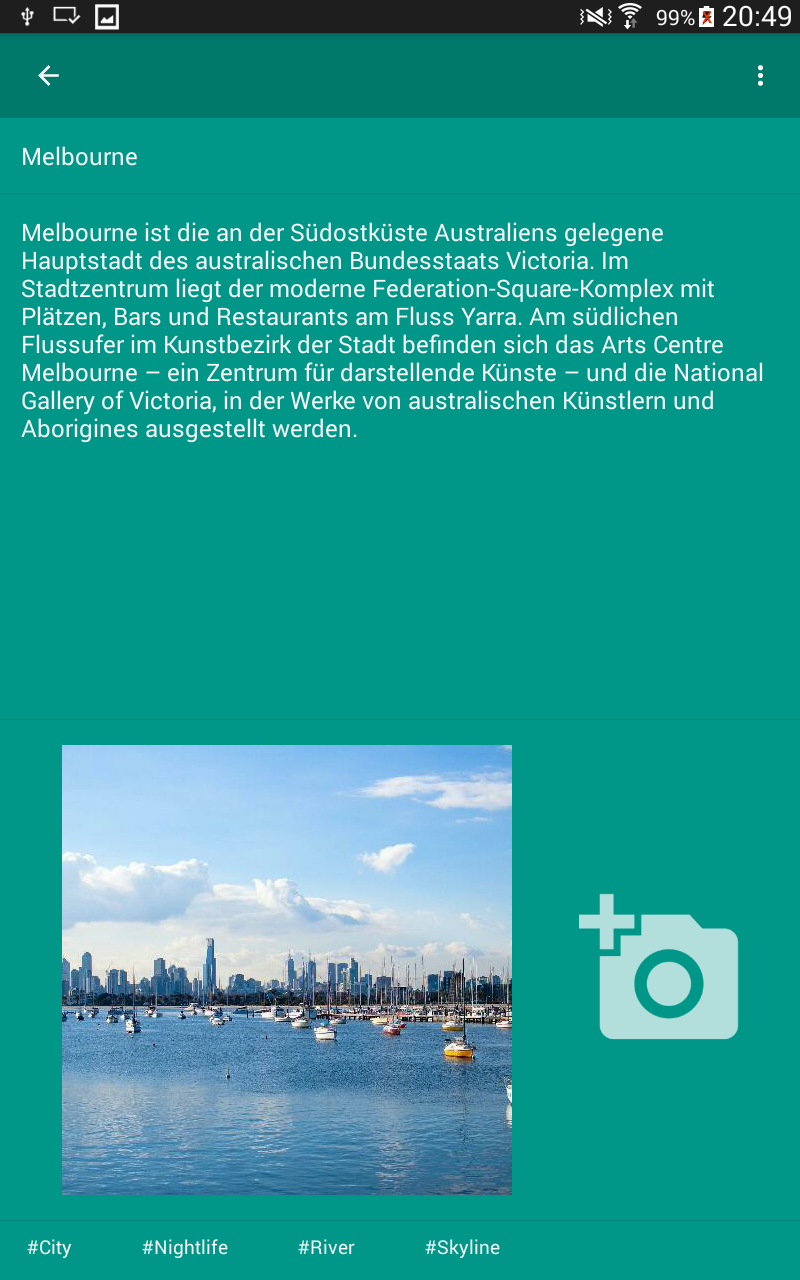
\includegraphics[height=20cm]{img/note_portrait.png}\\ % Pfad
\source{Screenshot aus der Benutzeroberfläche} % Quelle
\end{minipage}
\end{figure}

\subparagraph{Landscape-Ansicht}
Wird das Gerät gedreht und damit in die Landscape Ansicht gewechselt, wird die Ansicht etwas anders dargestellt. Primär wird hier die Bilderansicht auf die rechte Seite verschoben, um die Breite des Displays auszunutzen. Von nun an kann hier vertikal gescrollt werden und die Option zum Hinzufügen von neuen Bildern befindet sich an unterster Stelle.

Zusätzlich lässt sich hier Erkennen, dass die Ansicht jeweils die Hauptfarbe und die Akzentfarbe aus dem Note-Objekt übernimmt. Die Farbe wird zufällig beim Anlegen einer Notiz aus einer Vorauswahl ausgewählt und im Objekt gespeichert. Hier ist nun als Beispiel eine andere Farbgebung dargestellt.

\begin{figure}[H]
\centering
\begin{minipage}[t]{1\textwidth} % Breite, z.B. 1\textwidth		
\caption{Note Landscape-Ansicht} % Überschrift
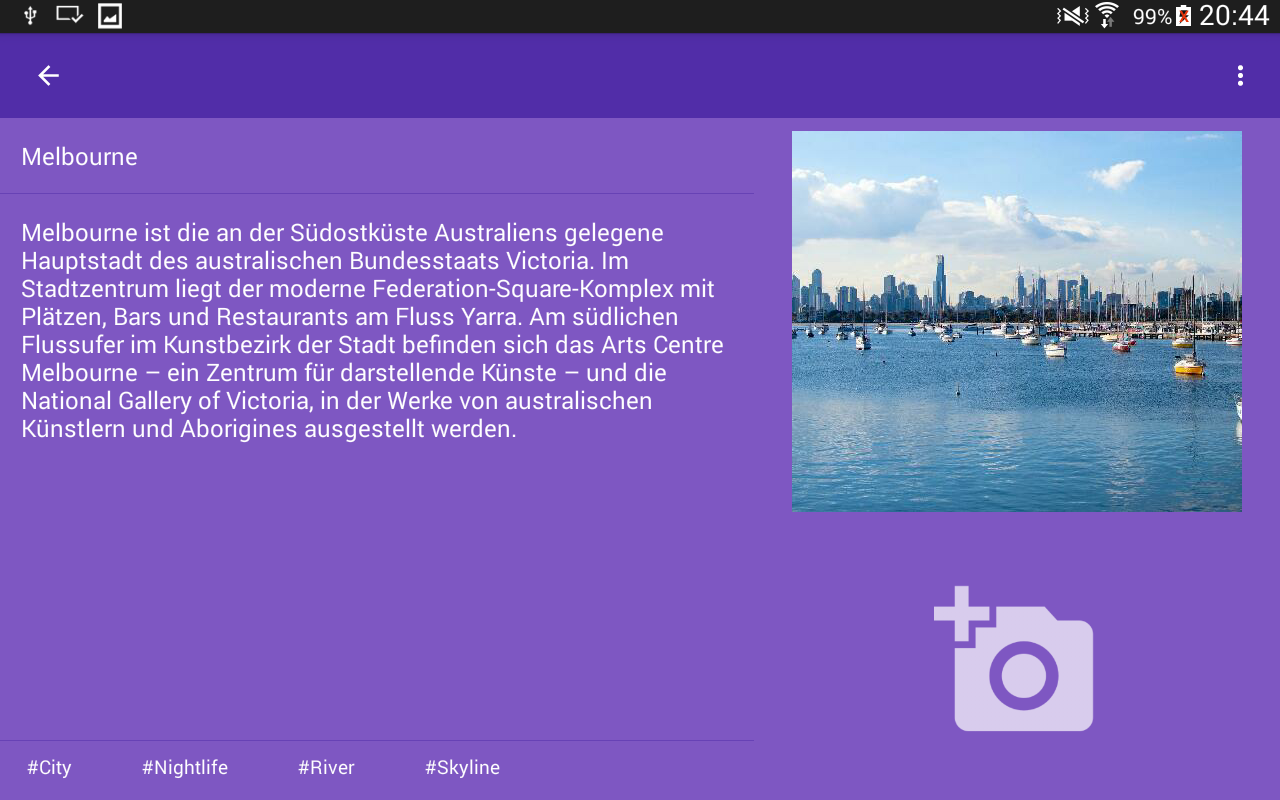
\includegraphics[width=1 \textwidth]{img/note_landscape.png}\\ % Pfad
\source{Screenshot aus der Benutzeroberfläche} % Quelle
\end{minipage}
\end{figure}

\subparagraph{Hinzufügen eines Bildes}
Falls der Nutzer das Icon zum Hinzufügen eines Bildes anklickt, gibt es zwei verschiedene Möglichkeiten, welche eintreten können. Falls das Gerät eine Kamera besitzt, wird der in der Abbildung dargestellte Dialog aufgerufen, damit der Nutzer sich entscheiden kann, ob ein Bild aus direkt aus der Kamera oder aus der Galerie importiert werden soll. Ist dies nicht der Fall, wird direkt die Androideigene Galerieimportfunktion gestartet. Für die Kamera wird ebenfalls eine Androideigene Funktion verwendet.

Nach Import des Bildes wird dies in der Bilderzeile angezeigt.

\begin{figure}[H]
\centering
\begin{minipage}[t]{1\textwidth} % Breite, z.B. 1\textwidth		
\caption{Note Dialog zum Hinzufügen eines Bildes} % Überschrift
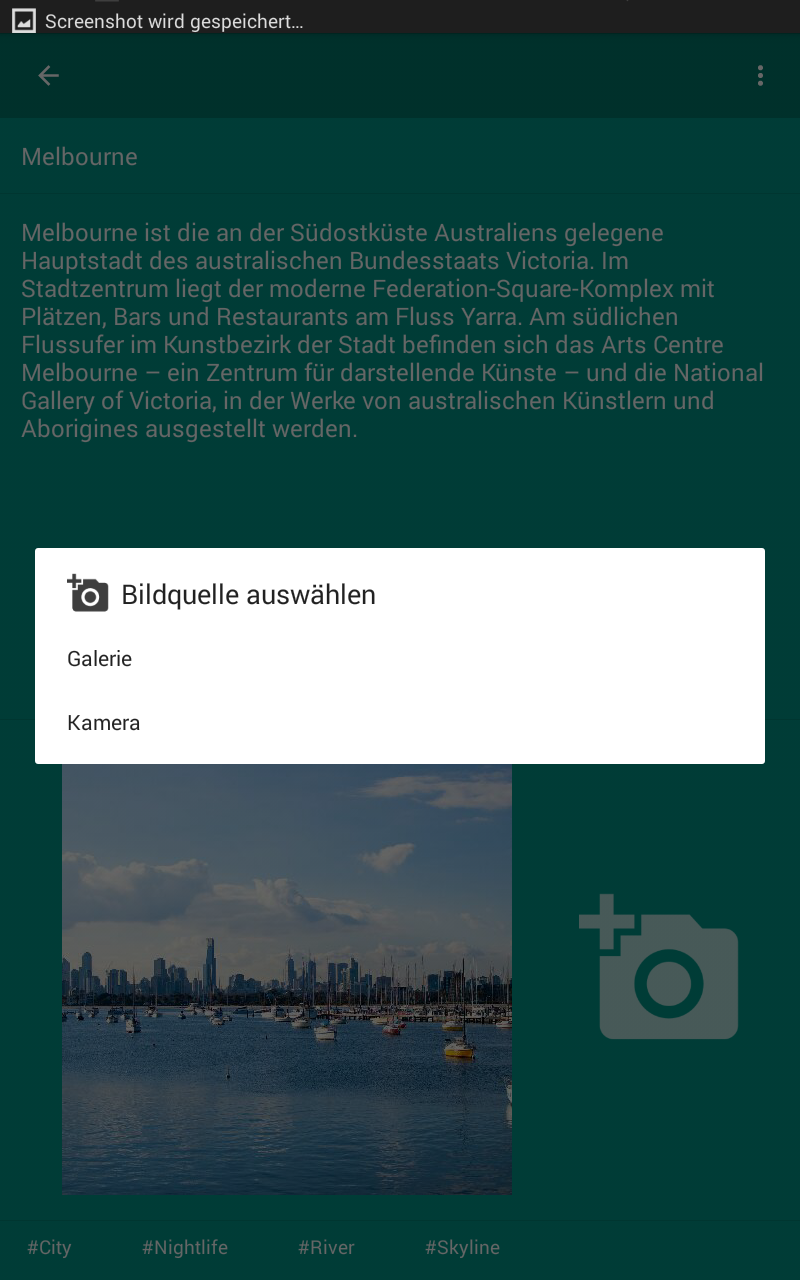
\includegraphics[height=20cm]{img/note_addImage}\\ % Pfad
\source{Screenshot aus der Benutzeroberfläche} % Quelle
\end{minipage}
\end{figure}

\subparagraph{Großansicht eines Bildes}
Wenn der Benutzer ein Bild auswählt, wird dieses im Großformat angezeigt. Dazu wird ein AlertDialog aufgerufen und mit dem Bild, welches in voller Größe aus der Datenbank geladen wird, gefüllt. Zusätzlich kann durch Wischgesten zwischen den Bildern gewechselt werden. Durch eine horizontale Wischgeste, das Klicken außerhalb des Bildbereiches oder das Betätigen des Zurück-Buttons wird die Ansicht geschlossen.

Das Bild füllt dabei den Bildschirm entsprechend eines in den Konstanten der Note-Activity festgelegten Wertes aus (in diesem Falle zu 95 Prozent). Falls das Display gedreht wird und zu dem Zeitpunkt ein Bild in Großansicht angezeigt wird, wird dieses den neuen Bildschirmverhältnissen angepasst.

\begin{figure}[H]
\centering
\begin{minipage}[t]{1\textwidth} % Breite, z.B. 1\textwidth		
\caption{Note Bildansicht} % Überschrift
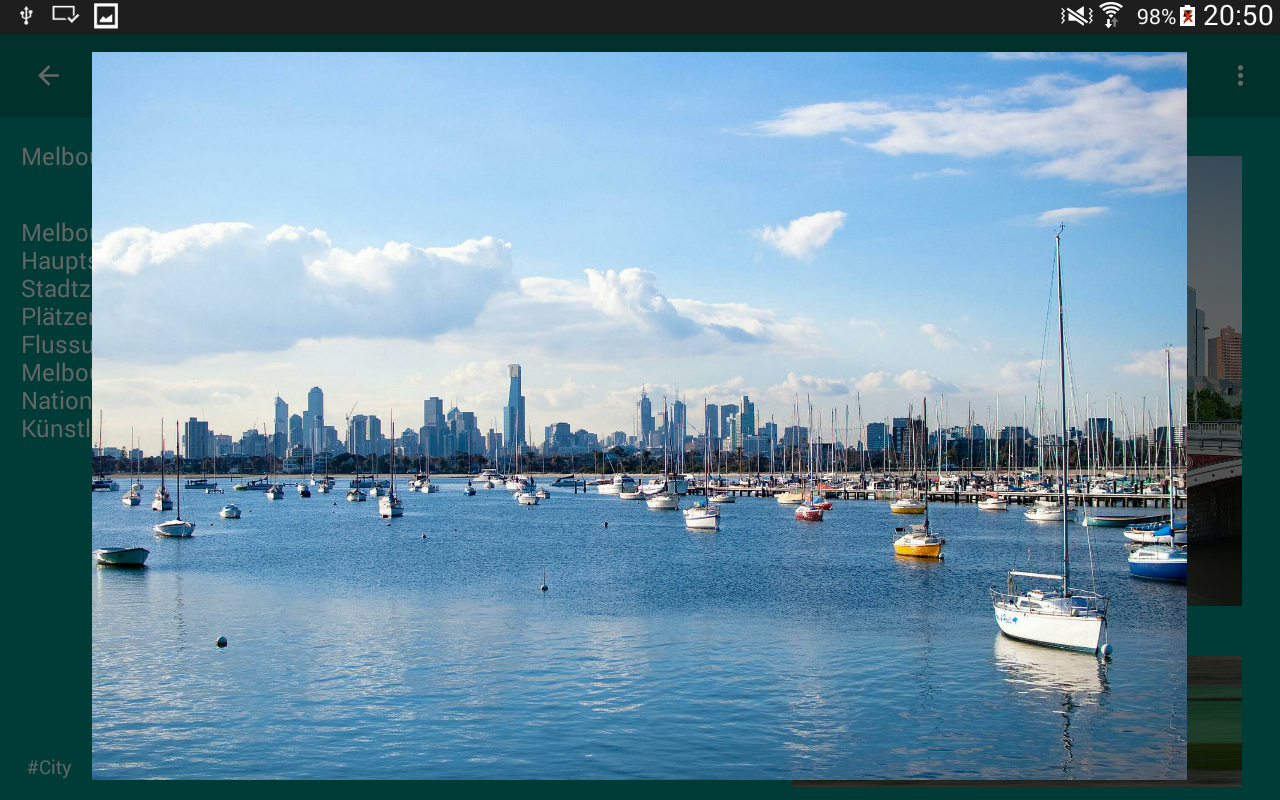
\includegraphics[width=1 \textwidth]{img/note_imageOverlay_landscape}\\ % Pfad
\source{Screenshot aus der Benutzeroberfläche} % Quelle
\end{minipage}
\end{figure}

\subparagraph{Toolbarmenü}
Über die Drei Punkte in der Toolbar kann das Menü aufgerufen werden, in welchem der Nutzer die Notiz extern teilen oder die Notiz löschen kann.

\begin{figure}[H]
\centering
\begin{minipage}[t]{1\textwidth} % Breite, z.B. 1\textwidth		
\caption{Note Toolbarmenü} % Überschrift
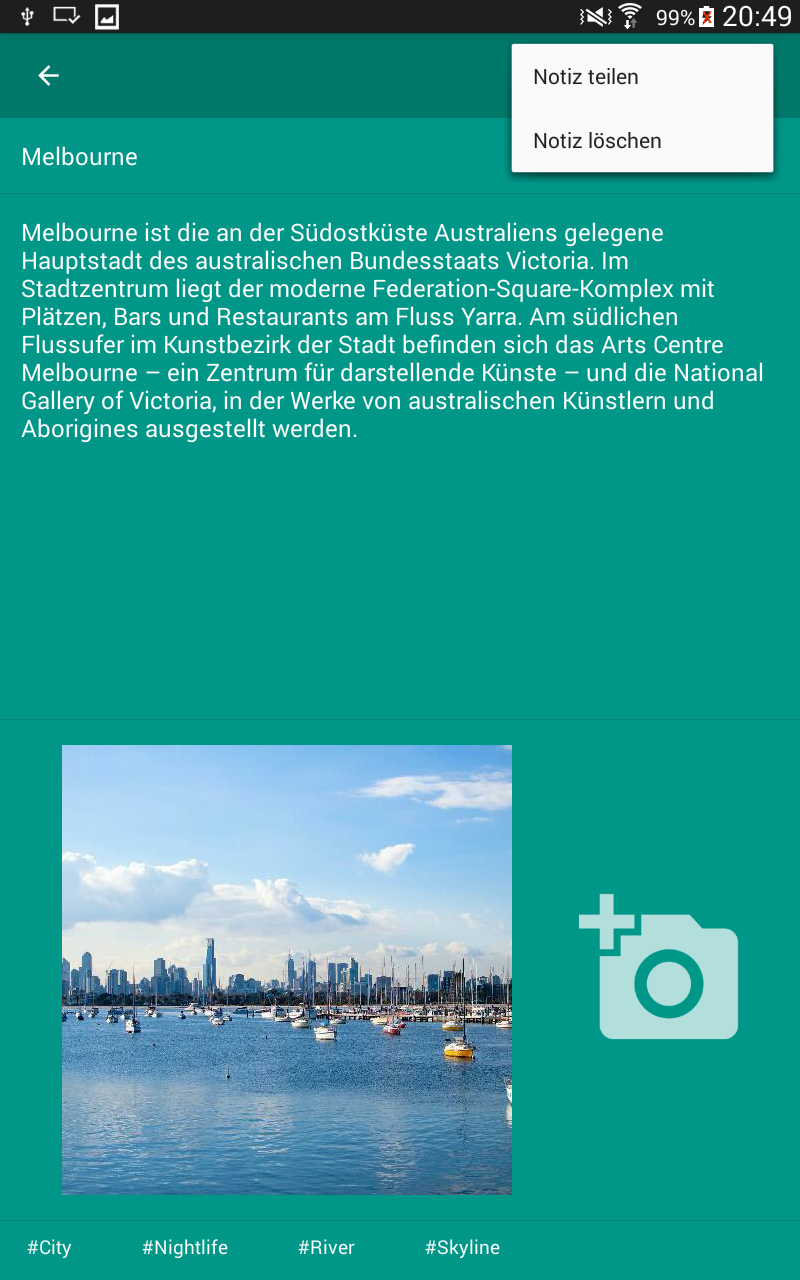
\includegraphics[height=20cm]{img/note_toolbarMenu}\\ % Pfad
\source{Screenshot aus der Benutzeroberfläche} % Quelle
\end{minipage}
\end{figure}

\paragraph{Use Case (Joscha Nassenstein)}
Der Use-Case dieser Activity besteht darin, sämtliche Attribute einer Notiz einpflegen beziehungsweise anpassen zu können. Der Funktionsumfang wurde bereits in dem vorangegangenen Kapitel Aufgabe und Funktion dargestellt.

Im Folgenden ist ein Use-Case Diagramm abgebildet, welche diese Funktionen zusammenfasst. Auf die Bedingung der extend-Pfeile wurde hierbei zur Erhöhung der Übersichtlichkeit verzichtet, da dies stets die entsprechende Benutzereingabe in Form eines Klicks auf die Fläche darstellt.

\begin{figure}[H]
\centering
\begin{minipage}[t]{1\textwidth} % Breite, z.B. 1\textwidth		
\caption{Note Use-Case Diagramm} % Überschrift
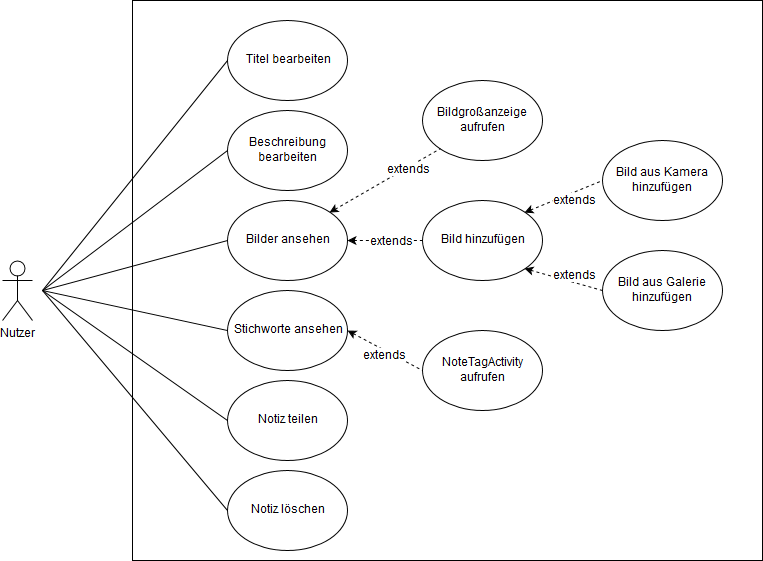
\includegraphics[width=1 \textwidth]{img/noteUseCase}\\ % Pfad
\source{Erstellt von Joscha Nassenstein} % Quelle
\end{minipage}
\end{figure}

\paragraph{Datenstruktur und -typen}
Die Notiz-Activity wird aus der Overview-Activity mittels eines Intents gestartet, welcher, falls die Notiz bereits besteht und keine neue Notiz angelegt werden soll, die jeweilige ID der Notiz übergibt, damit darüber auf die Datenbank zugegriffen werden kann. Die Klasse NoteActivity ist aus der Klasse AppCompatActivity abgeleitet und überschreibt die für die Funktionen relevanten Methoden dieser Klasse und initialisiert die im Nachfolgenden angesprochenen Verwaltungsklassen NoteData, NoteGui sowie NoteApplicationLogic.

\subparagraph{Restruktrierung der Pakete (Jan Beilfuß)}
Als bereits ein Großteil des Funktionsumfangs der Notiz-Activity implementiert war, gab es eine einzelne NoteData-Klasse und eine NoteApplicationLogic-Klasse. Alle Klassen der Notiz-Activity befanden sich in einem Paket.

Die Klassen NoteData und NoteApplicationLogic enthielten eine eine Vielzahl von Methoden mit unterschiedlichend fachlichen wie technischen Funktionen. Die Länge der beiden Klassen von 200 bis 300 Zeilen machte diese unübersichtlich. Als Folge dessen sinkt die Erweiterbarkeit und der Aufwand bei der Fehlerfindung steigt.

Es wurden folgende Maßnahmen getroffen, um die beschriebene Problemstellung zu lösen. Zu einen wurde im Paket note die drei Pakete data, logic und gui angelegt. Diese wurden weiter in Unterpakete aufgeteilt, sodass garantiert war, dass nicht mehr als sechs bis sieben Klassen im selben Paket liegen. Ebenfalls wurden die Klassen aufgeteilt und dann nach ihrer Funktion in die entsprechenden Pakete einsortiert.

Durch die ergriffenene Maßnahmen konnte bei der Weiterentwicklung der Applikation jeweils ein schneller Einstieg gefunden werden. Weiterhin konnte die gewählte Struktur flexibel für Implementierungen, die aus dem Debuggingprozess hervorgegangen sind, angepasst und erweitert werden.

\subparagraph{Data-Paket (Joscha Nassenstein)}
Das Data-Paket beinhaltet alle Klassen, welche für die Datenhaltung zuständig sind. Diese Funktionen werden zentral von der NoteData-Klasse verwaltet. Das Paket ist in Backend-orientierte und Benutzeroberflächen-orientierte Klassen aufgeteilt, um auch hier für eine Differenzierung zu sorgen. Zu den Backend-orientierten Klassen zählen dabei alle Klassen, welche für das asynchrone Laden der Notiz, insbesondere der Bilder, sorgen, um die Performance dieser Ansicht zu optimieren. Die Benutzeroberflächen-orientierten Datenklassen bestehen einer Klasse, welche für das Importieren der Bilder und das anschließende Bearbeiten, insbesondere in Bezug auf die Vorschaugröße, zuständig sind.

\subparagraph{GUI-Paket (Joscha Nassenstein)}
Innerhalb des GUI-Paket sind alle Klassen einsortiert, welche Views beinhalten, welche auf der Benutzeroberfläche dargestellt werden. Die NoteGui-Klasse repräsentiert die Struktur des Layouts und damit alle einzelnen Komponenten, um diese korrekt zu initialisieren und auf einzelne Views zugreifen zu können. Des Weiteren ist eine Klasse für die Darstellung eines ausgewählten Bildes in Form eines Overlays sowie Klassen für die Einsortierung der einzelnen Vorschaubilder in das allgemeine Notiz-Layout erstellt worden.

\subparagraph{Logic-Paket (Joscha Nassenstein)}
Das Paket, welches die Logik der Note-Activity beinhaltet, ist mit Abstand das umfangreichste der drei Pakete. Zunächst sind hier alle Listener- und Watcher Klassen beinhaltet, welche bei Klicken eines bestimmten Elements, darunter Views (auch Bilder) oder bestimmte Menüoptionen, sowie bei der Eingabe von Texten in den Titel und die Beschreibung bestimmte Aktionen ausführen. Eine Klasse ist zusätzlich für die Initialisierung dieser zuständig, eine weitere für das Ausführen der damit verbundenen Aktionen.

Die NoteApplicationLogic-Klasse ist die zentrale Logik-Klasse in der Note-Activity. Von hier aus werden die anderen Klassen, welche spezifische Aufgaben übernehmen, initialisiert und angesprochen. Zu den Funktionen letzterer Klassen gehören dabei die Verwaltung der asynchronen Ladelogik, eine Klasse zur Verwaltung der Galerie-Import Funktion, eine Klasse zur Erneuerung der Benutzeroberfläche, eine Klasse für die Detailanzeige von Bildern sowie eine Klasse für die Verwaltung der Navigation zwischen der Note-Activity und den damit verbundenen anderen Activities. Die Note-Activity interagiert neben der Overview-Activity auch mit der NoteTag-Activity zur Verwaltung der Stichwortliste sowie mit den von Android bereitgestellten Kamera- und Galerie-Activities. 

\begin{figure}[H]
\centering
\begin{minipage}[t]{1\textwidth} % Breite, z.B. 1\textwidth		
\caption{Darstellung der Paketstruktur} % Überschrift
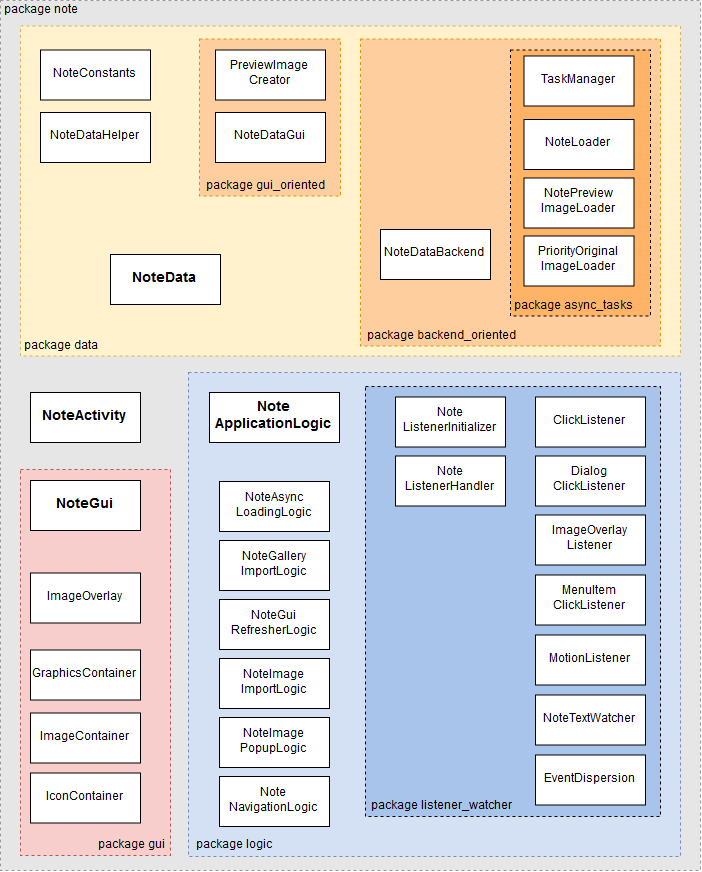
\includegraphics[width=1 \textwidth]{img/notePackageDiagram}\\ % Pfad
\source{Erstellt von Joscha Nassenstein} % Quelle
\end{minipage}
\end{figure}

\paragraph{Dokumentation des Quelltextes der Activity}
Im Nachfolgenden sind die einzelnen Klassen der \textit{Note-Activity} mit den jeweiligen wichtigsten Funktionen kurz beschrieben. In einem Beispiel ist ein Quellcodeausschnitt beigefügt.
\subparagraph{Klasse: NoteActivity (Joscha Nassenstein)}
Diese Klasse ist der zentrale Einstiegspunkt der Note-Activity und ist aus der AppCompatActivity-Klasse abgeleitet. Hier werden einige Methoden letzterer überschrieben und an die eigenen Anforderungen angepasst.

\textit{onCreate}:\\
In dieser Methode wird die im Intent übergebene ID ausgelesen und anhand dessen die NoteData-Klasse initialisiert. Zusätzlich werden NoteGui, NoteApplicationLogic und EventDispersion initialisiert. Falls keine ID übergeben wurde, wird die Tastatur eingeblendet und die NoteGui-Klasse mit dem Parameter pNewNote = true initialisiert, wodurch das Titelfeld zur direkten Eingabe durch den Benutzer fokussiert wird.

\textit{onActivityResult}:\\
An dieser Stelle wird das Ergebnis einer zuvor gestarteten externen Activity abgefangen und an die NoteApplicationLogic weitergegeben, wo das Ergebnis weiterverarbeitet werden kann.

\textit{onCreateContextMenu}:\\
Diese Methode wird jeweils für die Erstellung des Kontextmenüs innerhalb der Activity und in der Toolbar überschrieben. Die Methoden unterscheiden sich dabei durch den Rückgabetyp und den Parameter. Die Erstellung des Kontextmenüs findet letztlich in der Klasse EventDispersion statt.

\textit{onContextItemSelected}:\\
Hier wird ebenfalls die entsprechende Methode in EventDispersion aufgerufen.

\textit{onConfigurationChanged}:\\
Diese Methode wird aufgerufen, falls die Konfiguration des Gerätes, beispielsweise die Ausrichtung, verändert wird. Normalerweise wird bei einer Konfigurationsänderung die aktuelle Instanz der Activity beendet und eine neue Instanz aufgerufen. Dies wird jedoch durch die explizite  Einstellung im AndroidMainfest verhindert, damit hier ein eigener Ablauf implementiert werden kann. Konkret wird die Datenklasse erhalten, um weiterhin den aktuellen Stand der Daten zur Verfügung zu stellen. Die Oberfläche der Activity wird hingegen neu erstellt, da sich einige Elemente ändern. Dazu zählt primär der horizontale Scrollview, welcher in der Landscape-Ansicht einem Vertikalen weichen soll. Zusätzlich wird die entsprechende Methode in der NoteApplicationLogic aufgerufen, um weitere Aktionen durchzuführen.

\subparagraph{Klasse: NoteConstants (Jan Beilfuß)}
Diese Klasse enthält alle Konstanten, die in der Programmierung der Notiz-Activity Verwendung finden. Dazu gehören IDs und Requestcodes für den Datenaustausch mit den aus der Notiz-Activity aufgerufenen Intents Gallery, Kamera und NoteTagActivity, aber auch Skalierungsfaktoren und Größen, die in der Gui verwendet werden.

\subparagraph{Klasse: NoteDataHelper (Jan Beilfuß)}
Diese Klasse hat den Zweck Methoden zu bündeln, welche nicht am direkten Datenaustausch mit dem Backend oder Gui zu tun haben. Dazu zählt beispielsweise eine Methode, um zu checken, ob das gehaltene Notiz-Objekt lediglich mit default-Werten gefüllt ist.

\textit{isSaveable}:\\
 Diese Methode prüft, ob der Titel und die Beschreibung leere Strings sind. Weiterhin wird geprüft, ob die enthaltenen Listen tags und pictures leer sind. Sind alle Strings und Listen leer, wird das Objekt aus der Datenbank gelöscht und false zurückgegeben. Dadurch soll verhindert werden, dass leere Notiz-Kacheln in der Overview-Activity angezeigt werden.

\subparagraph{DATA}
\subparagraph*{Klasse: NoteData (Joscha Nassenstein)}
Die NoteData-Klasse spiegelt die zentrale Datenverwaltungsklasse wieder, aus der die backend- beziehungsweise benutzeroberflächen-bezogenen Datenklassen angesprochen werden.

\textit{shareNote}:\\
Diese Methode wird aufgerufen, falls der Benutzer im Kontextmenü die Option des Teilens ausgewählt hat. Von hier aus wird die shareNote-Methode im ShareModule aufgerufen.

\subparagraph*{Klasse: NoteDataBackend (Jan Beilfuß)}
In dieser Klasse werden alle Datenfunktionen gebündelt, welche mit dem Backend interagieren. Weiterhin wird hier die Liste der Bilder gehalten, welche beim Speicher zu löschen sind. Wenn der Nutzer beispielsweise ein Bild löscht und dann die App ohne speichern schließt, ist das Bild beim nächsten Laden im Vergleich zum direkten Löschen noch vorhanden.

\textit{deleteImage}:\\
Diese Methode entfernt das zu löschende Bild aus dem Note-Objekt und fügt dieses der Liste mit den zu löschenden Bildern hinzu.

\textit{triggerOriginalImageLoad}:\\
Diese Methode ruft im Taskmanager eine Funktion auf, um ein Bild in voller Auflösung im Hintergrund nachzuladen.

\textit{setColors}:\\
Diese Methode lädt die Haupt- und die Akzentfarbe zu dem Notizobjekt, dessen ID übergeben wurde und setzt diese in dem in NoteData gehaltenenen Notizobjekt.

\textit{executeSaveRoutine}:\\
Diese Methode bildet den Prozess der persistenten Speicherung in der Notiz-Activity ab. Zu erst wird das persistente Löschen der während der Laufzeit in der Oberfläche gelöschten Bilder durchgeführt. Darüber hinaus wird geprüft, ob die Notiz komplett leer ist. Wenn dies der Fall ist wird diese gelöscht, andernfalls wird sie in der Datenbank gespeichert. 

\textit{finallyDeleteImages}:\\
Diese Methode geht über alle Image-Objekte in der Liste mit den zu löschenden Bildern und übergibt diese der Delete-Methode im ImageService. Dadurch werden die Bilder im Dateisystem gelöscht.

\textit{deleteNote}:\\
Diese Methode wird aufgerufen, wenn man die Notiz in der Datenbank löschen möchte. Wenn das NoteObjekt existiert, wird dessen ID der Delete-Methode im Delete-Service aufgerufen und die ID übergeben.

\textit{loadNote}:\\
Diese Methode wird im Erstellungprozess der Notiz-Activitiy aufgerufen und veranlasst das Laden des Notizobjektes. Dafür wird im Taskmanager die Methode loadNote aufgerufen.

\textit{deleteImageFromDisk}:\\
Diese Methode löscht ein einzelnes Bild im Speicher. Sie wird aufgerufen, um die Datei, welche temporär für die Kamera-Activitiy angelegt wurde zu löschen. 

\textit{saveImage}:\\
 Diese Methode speichert ein übergebenes Bild. Sie wird verwendet nachdem eine Bitmap aus der Note oder Kameraactivity geladen und mit einer ID versehen wurde, um diese im Datenordner der Applikation abzulegen.

\subparagraph*{Klasse: TaskManager (Jan Beilfuß)}
Diese Klasse verwaltet den Einsatz aller asynchrone Tasks, die zum Laden von Daten aus der Datenbank und dem Dateisystem verwendet werden. 

\textit{triggerOriginalImagePriorityLoad}:\\
Diese Methode erzeugt ein Objekt der Klasse PriorityOriginalImageLoader. Über dieses Objekt wird das Bild zu dem übergebenen Index in originaler Größe asynchron geladen.

\textit{loadPreviewImages}:\\
Diese Methode erzeugt ein Objekt der Klasse NotePreviewImageLoader. Über dieses Objekt wird das Bild zu dem übergebenen Index in Vorschaugröße asynchron geladen.

\textit{loadNote}:\\
Diese Methode erzeugt ein Objekt der Klasse NoteLoader. Über dieses Objekt wird das Noteobjekt zu der übergebenen ID asynchron geladen.

\subparagraph*{Klasse: NotePreviewImageLoader (Jan Beilfuß)}
Diese Klasse erzeugt einen asynchrone Task der Klasse LoadPreviewImageTask, welche von AsyncTask erbt.

\textit{loadPreviewImage}:\\
Diese Methode erzeugt den asynchronen Task und führt diesen aus. In der Methode \textit{doInBackground} wird eine Kopie des Image-Objektes aus dem NoteObjekt angefertigt und in diese das gewünschte Vorschaubild geladen. Nach dem Laden wird in \textit{onPostExecute} das Bild aus dem Noteobjekt gelöscht, falls keine Bitmap geladen werden konnte, oder andernfalls das Bild über die Methode \textit{addAsyncPreviewImage} in die Note Activity geladen.

\subparagraph*{Klasse: PriorityOriginalIMageLoader (Jan Beilfuß)}
Diese Klasse erzeugt einen asynchrone Task der Klasse LoadOriginalImageTask, welche von AsyncTask erbt.

\textit{loadOriginalImage}:\\
Diese Methode erzeugt den asynchronen Task und führt diesen aus. In der Methode \textit{doInBackground} wird das Bild in originaler Größe geladen. Vor dem Laden wird in \textit{onPreExecute} der Ladespinner gestartet. Nach dem Laden wird in \textit{onPostExecute} das Bild aus dem Noteobjekt gelöscht, falls keine Bitmap geladen werden konnte, oder andernfalls das Bild über die Methode \textit{addAsyncPreviewImage} in die Note Activity geladen, der Ladespinner gestoppt und das Bild als Popup angezeigt.

\subparagraph*{Klasse: NoteLoader (Jan Beilfuß)}
Diese Klasse erzeugt einen asynchrone Task der Klasse LoadNoteTask, welche von AsyncTask erbt.
\textit{loadNote}:\\
Diese Methode erzeugt den asynchronen Task und führt diesen aus. In der Methode \textit{doInBackground} wird das Note-Objekt aus der Datenbank geladen. Nach dem Laden wird in \textit{onPostExecute} das Note-Objekt in NoteData gesetzt und die Methode \textit{dataToGui} ausgeführt, um dieses in der Oberfläche anzuzeigen.

\subparagraph*{Klasse: NoteDataGui (Jan Beilfuß)}
In dieser Klasse werden alle Datenfunktionen gebündelt, welche Datenänderungen durch Nutzer-Interaktion mit der Oberfläche erzeugen. Weiterhin wird hier die Liste der Bilder gehalten, welche in der Oberfläche als Vorschaubilder angezeigt werden.

\textit{addImageFromGallery}:\\
Diese Methode bekommt die Bitmap des aus der Gallerie importierten Bildes übergeben. Daraus wird über die Methode \textit{addPreviewImageFromOriginal} ein Vorschaubild erzeugt und dieses der Liste mit Vorschaubildern hinzugefügt. Weiterhin wird das Originale Bild in den applikationseigenen Ordnern abgespeichert.

\textit{addPreviewImageFromOriginal}:\\
Diese Methode erzeugt aus einem originalen Bild ein Vorschaubild und fügt dieses der klasseneigenen Liste an Vorschaubildern hinzu.

\textit{addImageFromCamera}:\\
Diese Methode fügt das aus der Kamera-Activity übergebene Bild hinzu. Dazu wird die Methode \textit{addImageFromGallery} aufgerufen und zusätzlich die zuvor temporär erstellte Datei gelöscht.

\textit{getOriginalImage}:\\
Diese Methode wird aufgerufen, wenn man auf ein Bild klickt, um dieses in originaler Größe zu laden. Sofern dieses nicht in dem Note-Objekt in NoteData gespeichert ist, wird in NoteDataBackend die Methode \textit{triggerOriginalImageLoad} aufgerufen, um dieses aus dem Dateisystem zu laden.

\textit{deleteImage}:\\
Diese Methode wird aufgerufen, wenn der Nutzer in der Oberfläche ein Bild löchen möchte. Dieses Bild wird aus der Liste an Vorschaubildern gelöscht und die Oberfläche aufgefrischt.

\textit{refreshImages}:\\
Diese Methode ruft in der NoteGuiRefresherLogic die Methode \textit{refreshImages} auf, um die Gui bei Änderungen im Datenbestand zu aktualisieren.

\textit{getLatestImage}:\\
Diese Methode gibt das letzte Bild der Liste an Vorschaubildern zurück. Dies wird verwendet, damit man dieses beim Asynchronen Laden als einzelnes Bild animiert dem Layout hinzufügen kann.

\subparagraph*{Klasse: PreviewImageCreator (Joscha Nassenstein)}
Diese Klasse beinhaltet die Methode, um ein Bild auf Vorschaugröße zu skalieren.

\textit{getPreviewImage}:\\
Erstellt aus dem Originalbild, welches als Parameter übergeben wird, ein verkleinertes und im Seitenverhältnis angepasstes Bild. In der aktuellen Form wird dabei ein quadratisches Bild in Größe der entsprechenden Konstanten in NoteConstants erstellt.

\subparagraph{GUI}
\subparagraph*{Klasse: NoteGui (Joscha Nassenstein)}
Die NoteGui-Klasse beinhaltet die Benutzeroberflächenelemente als Attribute, wodurch auf diese zugegriffen werden kann. Zusätzlich werden von hier aus die Animationen für das asynchrone Laden der Bilder gesteuert.

\textit{initiateOrientationDepententViews}:\\
Die Layouts für den Portrait- und den Landscapemodus beinhalten in der Note-Activity verschiedene Elemente, um eine optimale Darstellung zu ermöglichen. Einerseits gibt in der Portrait-Ansicht einen Separator mehr als in der Landscape-Ansicht, andererseits ist das ScrollView in der Portrait-Ansicht horizontal und in der Landscape-Ansicht vertikal scrollbar. Um diese Views entsprechend der Orientation des Gerätes auszurichten, wird in dieser Methode die aktuelle Orientation abgefragt und entsprechend des Ergebnisses die Variablen initialisiert.

\textit{setColors}:\\
Da jede Notiz zwei verschiedene Farben enthält, werden in dieser Methode die Benutzeroberflächenelemente anhand der Farben aus der Notiz angepasst.

\textit{formatTags}:\\
In dieser Methode werden die Stichwörter aus der Notiz für die Ansicht formatiert.

\subparagraph*{Klasse: GraphicsContainer (Joscha Nassenstein)}
Diese Klasse stellt die Überklasse für die beiden nachfolgenden Klassen dar und beinhaltet ein LinearLayout, in welches ein Vorschaubild beziehungsweise ein Icon eingefügt werden kann. Dieses wird wiederum in den ScrollView der Note-Ansicht eingefügt. Das LinearLayout besitzt eine ID, welche für die Erkennung des zu löschenden Bildes bei der entsprechenden Benutzereingabe verwendet wird.

\subparagraph*{Klasse: ImageContainer (Joscha Nassenstein)}
Diese Klasse beinhaltet ein ImageView, in welches durch die nachfolgende Methode das entsprechende Vorschaubild eingefügt werden kann. Der ImageView kann von außerhalb der Klasse mithilfe eines Getters abgerufen werden, um in diesem spezifischen Falle eine Animation für das Erscheinen nach dem asynchronen Laden zu ermöglichen. Der ImageView wird im Konstruktor der Klasse ebenfalls für das Kontext-Menü registriert, um das Löschen eines Bildes zu ermöglichen.

\textit{initiateView}:\\
Anhand eines übergebenen Bildes wird ein imageView initialisiert und auf das LinearLayout aus der GraphicsContainer-Klasse gesetzt.

\subparagraph*{Klasse: IconContainer (Joscha Nassenstein)}
In dieser Klasse wird in der nachfolgenden Methode ebenfalls ein ImageView erstellt, hier jedoch mit einem Icon an Stelle eines Bildes. Der ImageView selbst wird hier nicht gehalten, da dieser nur temporär in der nachfolgenden Methode benötigt wird.

\textit{initiateView}:\\
Anhand des im Konstruktors übergebenen Icons wird der ImageView initialisiert und auf das LinearLayout aus der GraphicsContainer-Klasse gesetzt. Die Layout-Parameter werden anhand der aktuellen Orientierung ausgewählt, um eine unnötig breite Erscheinung des Layouts zu vermeiden.

\subparagraph*{Klasse: ImageOverlay (Joscha Nassenstein)}
In dieser Klasse wird anhand eines übergebenen Bildes und der aktuellen Displayeigenschaften ein AlertDialog erstellt, welcher das Bild im Großformat anzeigt.

\textit{display}:\\
Der bereits erwähnte AlertDialog wird mit dem übergebenen Bild und entsprechend der in der nachfolgenden Methode berechneten Größe erstellt und anschließend angezeigt.

\textit{calculateSize}:\\
Hier wird anhand der in die Klasse übergebenen aktuellen Displayeigenschaften, sprich der Displaygröße, das aktuelle Seitenverhältnis ausgerechnet. Dies wird ebenfalls für das Bild durchgeführt. Anschließend wird anhand verschiedener Vergleiche die optimale Bildgröße ermittelt, sodass das Bild in maximaler Größe angezeigt werden kann und der AlertDialog keine Ränder aufweist. Ermittelt wird diese Größe dadurch, dass überprüft wird, ob das Bild bei einer Skalierung zunächst die Breite oder die Höhe des Bildschirms überschreiten würde. Zusätzlich wird ein in NoteConstants vermerkter Füllfaktor berücksichtigt, welcher bestimmt, zu welchem Grad der Bildschirm mit dem Bild ausgefüllt werden soll.
Der Quellcode ist im Nachfolgenden dargestellt: 


\begin{figure}[H]
\centering
\begin{minipage}[t]{1\textwidth} % Breite, z.B. 1\textwidth		
\caption{Codebeispiel} % Überschrift
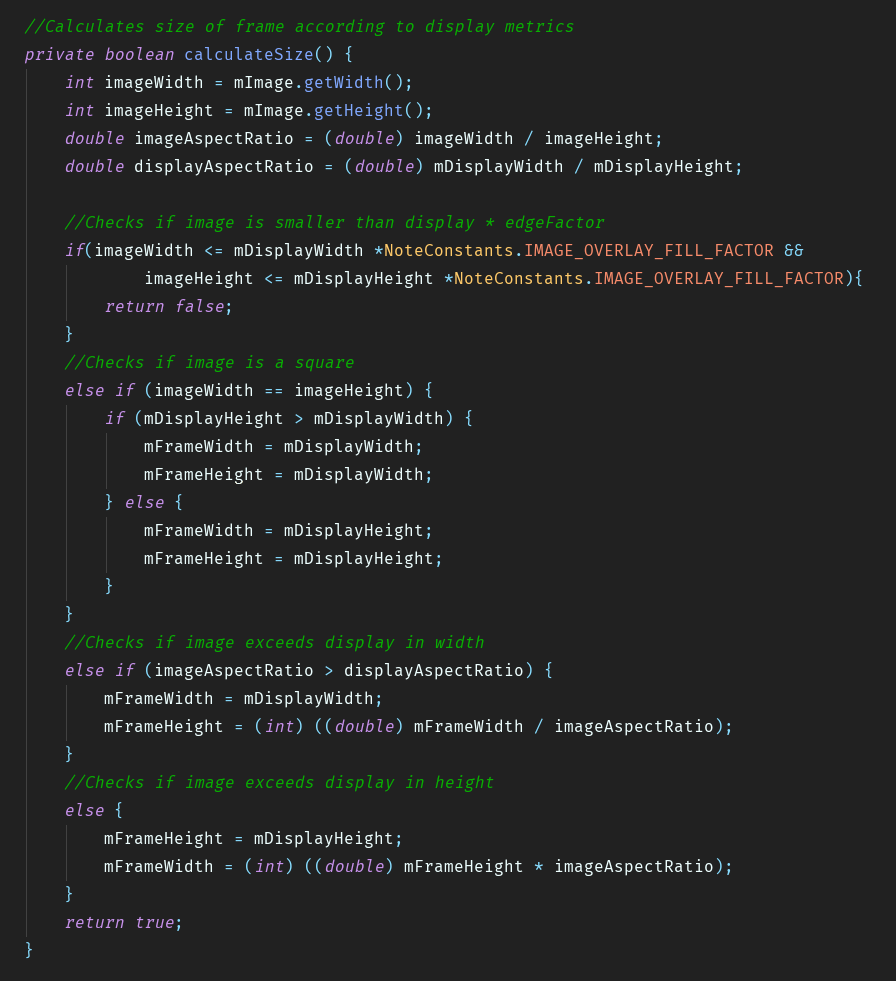
\includegraphics[width=1 \textwidth]{img/note_imageOverlayCodeExample}\\ % Pfad
\source{Screenshot aus der Entwicklungsumgebung} % Quelle
\end{minipage}
\end{figure}

\textit{changeOrientation}:\\
Bei einer Konfigurationsänderung wird in der NoteApplicationLogic stets überprüft, ob aktuell ein ImageOverlay angezeigt wird. Ist dies der Fall, wird diese Methode aufgerufen, um den aktuellen AlertDialog zu verwerfen und entsprechend der neuen Displayeigenschaften einen Neuen zu erstellen, damit der Bildschirm wieder maximal ausgefüllt wird.

\subparagraph{LOGIC}
\subparagraph*{Klasse: NoteApplicationLogic (Joscha Nassenstein)}
Diese Klasse stellt die zentrale Stelle für die Logik der Note-Activity dar und verwaltet die anderen Klassen, welche in diesem Paket zu finden sind.

\textit{onConfigurationChanged}:\\
Diese Methode wird aus NoteActivity aufgerufen, falls sich die Konfiguration der Geräts geändert hat. Anhand der neu übergebenen Gui-Klasse werden dabei die ClickListener neu gesetzt und die Benutzeroberfläche mit den bestehenden Daten aufgefüllt. Zusätzlich wird die Methode changeConfiguration in der ImagePopupLogic aufgerufen.

\subparagraph*{Klasse: ClickListener (Joscha Nassenstein)}
Die Klasse ClickListener implementiert das Interface View.OnClickListener und kann dementsprechend instanziiert auf ein View als OnClickListener gesetzt werden.

\textit{onClick}:\\
Hier wird die Methode aus der Basisklasse überschrieben und an die eigenen Anforderungen angepasst. Konkret wird überprüft, ob auf die Stichworte oder auf den Zurückpfeil in der Toolbar geklickt wurde, auf die jeweils ein ClickListener gesetzt wurde. Ist dies nicht der Fall, wird anhand der ID überprüft, ob auf ein Bild geklickt wurde und auf welches, um letztlich das Popup mit dem Bild anzuzeigen

\subparagraph*{Klasse: DialogClickListener (Joscha Nassenstein)}
Diese Klasse implementiert das Interface DialogInterface.OnClickListener und wird in diesem Falle auf das Menü zur Auswahl der Bildquelle gesetzt.

\textit{onClick}:\\
Hier wird ermittelt, ob die Option Galerie oder die Option Kamera ausgewählt wurde und dementsprechend die jeweilige Methode in der Klasse ImageImport aufgerufen.

\subparagraph*{Klasse: EventDispersion (Joscha Nassenstein)}
Diese Klasse ist für das Erstellen und das Behandeln des Kontextmenüs zuständig, welches hier auf ein Bild im ScrollView gesetzt wird, falls der Nutzer lange auf dieses drückt.

\textit{onCreateContextMenu}:\\
Hier wird das Menü auf den View gesetzt und die ID des Views gespeichert, um bei einer Auswahl der Option „Bild löschen“ die ID für das Bild zu haben, welches gelöscht werden soll.

\textit{onContextItemSelected}:\\
Wird ausgewählt, dass das Bild gelöscht werden soll, wird hier die entsprechende Methode in der NoteApplicationLogic anhand der zuvor gespeicherten ID aufgerufen.

\subparagraph*{Klasse: ImageOverlayListener (Jan Beilfuß)}
Diese Klasse implementiert das Interface DialogInterface.OnCancelListener.
textit{onCancel}
Diese Methode wird aufgerufen, wenn der Dialog, welchem der Listener hinzugefügt wurde durch den Nutzer geschlossen wird. Es werden dann zum einen alle Bitmaps, mit Bildern in Originalgröße aus dem Arbeitsspeicher gelöscht und das ImageOverlay ebenfalls auf null gesetzt, um den Speicherverbrauch zu optimieren.

\subparagraph*{Klasse: MenuItemClickListener (Joscha Nassenstein)}
Diese Klasse implementiert das Interface Toolbar.OnMenuItemClickListener und ist für das Behandeln der Optionen im Menü der Toolbar zuständig.

\textit{onMenuItemClick}:\\
Falls der Nutzer eine Option ausgewählt hat, wird hier die Methode onMenuItemClicked in der Klasse NoteClickHandler aufgerufen und das MenuItem als Parameter übergeben.

\subparagraph*{Klasse: MotionListener (Joscha Nassenstein)}
Die Klasse MotionListener implementiert das Interface View.OnTouchListener und wird hier als OnTouchListener auf den ImageView des Popups gesetzt, um Wischgesten erkennen zu können.

\textit{onTouch}:\\
Die Methode onTouch überschreibt die Methode der Basisklasse und ermittelt anhand des übermittelten MotionEvents, ob und falls ja, in welche Richtung gewischt wurde. Die minimale Distanz ist dabei in NoteConstants festgelegt. Anhand der Richtung wird bei Erfüllung dieses Kriteriums die jeweilige Methode in NoteImagePopupLogic aufgerufen. Bei einer horizontalen Wischgeste wird dabei das nächste bzw. vorherige Bild aufgerufen (falls dies existiert) und bei einer vertikalen Wischgeste wird das Overlay geschlossen.

\subparagraph*{Klasse: NoteListenerHandler (Joscha Nassenstein)}
Diese Klasse beinhaltet alle Methoden, welche aus den onClick-Methoden der Listener- bzw. Watcher-Klassen aufgerufen werden und bestimmte Aktionen ausführen.

\textit{onImageClicked}:\\
Diese Methode wird aufgerufen, falls auf ein Bild beziehungsweise das „Bild hinzufügen“-Icon im ScrollView geklickt wurde. In letzterem Falle wird das Importieren eines Bildes initialisiert. Falls ein Bild angeklickt wurde, wird das Popup zur Vollbildanzeige des Bildes initialisiert.

\textit{onTagsClicked}:\\
Falls der TextView, welcher die Stichworte enthält, angeklickt wurde, wird die Methode startTagActivity() in der NoteNavigationLogic aufgerufen, welche die neue Activity zur Verwaltung der Stichwörter startet.

\textit{onTextChanged}:\\
Hier wird, je nachdem, ob der Text im Titel oder in der Beschreibung geändert wurde, stets der aktuelle Stand in das Note-Objekt gespeichert.

\textit{onMenuItemClicked}:\\
Diese Methode wird aus dem menü der Toolbar heraus aufgerufen und ist je nach Auswahl dafür zuständig, den „Notiz teilen“-Vorgang aus dem ShareModule heraus zu starten beziehungsweise die Notiz zu löschen und zur Übersicht zurückzukehren (mittels der Methode returnToOverview() der NoteNavigationLogic).

\subparagraph*{Klasse: NoteListenerInitializer (Joscha Nassenstein)}
Diese Klasse hat den ClickListener der Note-Activity als Attribut enthalten und ist für dessen Initialisieren zuständig.

\textit{initListener}:\\
In dieser Methode wird der ClickListener auf die verschiedenen Views gesetzt. Zu den Views zählen das LinearLayout, welches im ScrollView die einzelnen Bilder und das Icon beinhaltet, sowie der TextView mit den Stichwörtern und der Zurück-Button der Toolbar. Zusätzlich werden auf die EditText-Views für Titel und Beschreibung jeweils ein TextWatcher gesetzt und der MenuItemClickListener auf das Toolbar-Menü gesetzt.

\subparagraph*{Klasse: NoteTextWatcher (Joscha Nassenstein)}
Der NoteTextWatcher implementiert das Interface android.text.TextWatcher und ist zur Speicherung von Eingaben in Titel und Beschreibung zuständig.

\textit{onTextChanged}:\\
Diese Methode überschreibt die entsprechende Methode der Basisklasse und ist dafür zuständig, die OnTextChanged-Methode im NoteClickHandler aufzurufen, falls ein Text geändert wurde, und die entsprechende CharSequence und den View, in welchem die Änderun stattgefunden hat, zu übergeben.

\subparagraph*{Klasse: NoteImageImportLogic (Joscha Nassenstein)}
In dieser Klasse sind die Funktionen beinhaltet, welche das Importieren von Bildern aus Kamera und Galerie anstoßen.

\textit{requestImageSource}:\\
In dieser Methode wird zunächst überprüft, ob das Gerät eine Kamera besitzt. Ist dies nicht der Fall, wird die Methode importImageFromGallery aufgerufen. Falls das Gerät eine Kamera besitzt, wird dem Nutzer ein Dialog angezeigt, welcher abfragt, ob der Benutzer ein Bild aufnehmen oder aus der Gallerie importieren möchte. Der DialogClickListener, welcher auf den AlertDialog gesetzt wird, erfasst die Benutzereingabe.

\textit{importImageFromCamera}:\\
In dieser Methode wird ein Intent erstellt, welcher anhand der Methode Activity.startActivityForResult die Android-eigene Kamera-Activity startet. Um die Aufnahme als Datei speichern zu können, wird durch den ImageService, welcher in den Activity-übergreifenden Klassen zu finden ist, eine Bilddatei erstellt (Methode: createImageFile) und die entsprechende Uri durch den Intent an die Kamera-Activity mitgegeben. In Android Version unter Android 6.0 („Marshmallow“) müssen diesem Intent zusätzlich zwei Flags mitgegeben werden, welche das Lesen und Schreiben dieser Uri erlauben und somit eine SecurityException vermeiden.
Die Kamera-Activity wird anhand eines in NoteConstants festgelegten, spezifischen RequestCodes gestartet, um das Ergebnis nach Rückkehr richtig zuordnen zu können.

\textit{importImageFromGallery}:\\
Hier wird ein Intent erstellt, in welchem nach Start der Activity ein Bild aus der Gallerie importiert werden kann. Da der Pfad zu dem jeweiligen Bild direkt aus dem Result extrahiert werden kann, muss hier keine Datei erstellt werden. Auch hier wird ein in NoteConstants spezifizierter Requestcode mitgegeben. 

\subparagraph*{Klasse: NoteAsyncLoadingLogic (Jan Beilfuß)}
Diese Klasse bündelt alle Methoden, welche beim asynchronen Nachladen von Bildern aufgerufen werden, um Veränderungen in der Oberfläche zu bewirken.

\textit{addAsyncPreviewImage}:\\
Diese Methode wird aus dem asynchronen Task LoadPreviewImageTask aufgerufen. Sie fügt das Bild der Liste an Vorschaubildern in NoteDataGui hinzu und lässt das Bild animiert in der Gui hinzufügen.

\textit{startLoadingSpinner}:\\
Diese Methode ruft in der Gui die Methode \textit{disableAll} auf. Dadurch werden die Texteingabefelder und das Tagfeld deaktiviert und reagieren nicht mehr auf Klick-Events. Weiterhin wird der Ladespinner angezeigt.

\textit{stopLoadingSpinner}:\\
Diese Methode ruft in der Gui die Methode \textit{enableAll} auf. Dadurch werden die Texteingabefelder und das Tagfeld wieder aktiviert und reagieren auf Klick-Events. Weiterhin wird der Ladespinner wieder ausgeblendet.

\subparagraph*{Klasse: NoteGalleryImportLogic (Jan Beilfuß)}
Diese Klasse bündelt alle Methoden, die den Bilderimport aus der Gallerie managen.

\textit{getPath}:\\
Diese Methode ermittelt aus dem Context und der aus der Gallery Intent zurückgegeben Uri den absoluten Pfad des ausgewählten Bildes. Ein Objekt der Klasse Cursor zeigt auf die entsprechende Datei, und gibt den Pfad dieser zurück. Im Anschluss wird dieses geschlossen und der Pfad zurückgegeben.

\textit{importImageFromGallery}:\\
Diese Methode bildet den gesamten Prozess ab, um ein Bild aus der Gallerie zu importieren. Beginnend beim Ermitteln des Pfades, der Kompression, falls das Bild zu groß ist und die Korrektur der Rotation. Danach wird in NoteData die Methode \textit{addImageFromGallery} aufgerufen, um das Bild den Datenhinzuzufügen und danach die Oberfläche aktualisiert.

\subparagraph*{Klasse: NoteGuiRefresherLogic (Joscha Nassenstein)}
Diese Klasse ist dafür zuständig, die Benutzeroberfläche zu aktualisieren, beispielsweise bei Aufruf der Activity und bei einer Konfigurationsänderung.

\textit{dataToGui}:\\
Aus dieser Methode heraus werden die Farben der Benutzeroberfläche gesetzt und anhand des Note-Objekts die Felder Titel, Beschreibung und Stichworte mit Inhalt gefüllt. Anschließend wird die nachfolgende Methode zur Erneuerung der Vorschaubilder aufgerufen.

\textit{refreshImages}:\\
In dieser Methode werden zunächst alle Views aus dem LinearLayout, welches im ScrollView der Activity die Bilder beinhaltet, gelöscht. Anschließend werden alle PreviewImages aus NoteData auf das LinearLayout gesetzt und jeweils mit einer ID und einem ClickListener versehen. Als letzter Schritt wird das „Bild hinzufügen“-Icon auf das LinearLayout gesetzt und ebenfalls mit einer ID und einem Clicklistener versehen.

\subparagraph*{Klasse: ImagePopupLogic (Joscha Nassenstein und Jan Beilfuß)}
In dieser Klasse wird das ImageOverlay erstellt und gestartet.

\textit{openImagePopup (Joscha Nassenstein)}:\\
In dieser Methode werden die aktuellen Displayeigenschaften abgefragt und anhand der aktuellen Maße das ImageOverlay erstellt und gestartet.

\textit{changeConfiguration (Jan Beilfuß)}:\\
Diese Methode wird relevant, wenn man ein Image-Popup geöffnet hat und den Bildschirm dreht. Über die neue Konfiguration kann man sich die Bildschirmmaße nach der Drehung in dp ausgeben lassen. Über die Pixeldichte wird Größe auf Pixel hochgerechnet und der Methode \textit{changeOrientation} des ImageOverlays mitgegeben. Diese erzeugt das Overlay dann auf die neue Displaygröße angepasst.

\textit{displayPreviousImage / displayNextImage }:\\
Falls eine Wischgeste von links nach rechts auf dem ImagePopup erkannt wurde, welche die Mindestdistanz in NoteConstants übertrifft, wird diese Methode ausgeführt. Hier wird überprüft, ob ein vorheriges Bild existiert. Falls dies der Fall ist, wird die Methode displayNewImage mit der neuen ID aufgerufen. In der Methode displayNextImage wird der gegenteilige Fall behandelt.

\textit{displaynewImage}:\\
Hier wird der aktuelle AlertDialog geschlossen, die geladenen Bitmaps zur Speicheroptimierung gelöscht und anschließend anhand der übergebenen ID ein neuer AlertDialog aufgerufen.

\subparagraph*{Klasse: NoteNavigationLogic (Joscha Nassenstein)}
In dieser Klasse werden alle Interaktionen mit anderen Activities gesteuert.

\textit{saveAndReturnToOverview}:\\
Hier wird die Methode executeSaveRoutine in NoteData ausgeführt und anschließend die NoteActivity beendet, wodurch der Nutzer zu der Übersicht zurückkehrt.

\textit{onActivityReturned}:\\
In dieser Methode wird anhand des übergebenen Requestcodes ermittelt, aus welcher zuvor gestarteten Activity das Ergebnis stammt. Zu den Activities gehören die Android Kamera- und Galeriefunktion sowie die TagActivity zur Verwaltung der Stichwörter. Anschließend wird das Ergebnis in anderen Logik-Klassen weiterverarbeitet. Im Falle der Stichwörter werden diese direkt in das Note-Objekt und die Oberfläche eingefügt.

\textit{startTagActivity}:\\
Hier wird der Intent erstellt, welcher für das Starten der TagActivity genutzt wird. Dem Intent werden die aktuelle Stichwortliste sowie die Farbe und die Akzentfarbe der Notiz mitgegeben. Anschließend wird die TagActivity gestartet.

\subsubsection{NoteTag Activity}
\fancyhead[L]{NoteTag Activity}
Aus der Notiz-Ansicht heraus kann man sich zwar die Stichwörter zu der jeweiligen Notiz ansehen, diese können jedoch nicht bearbeitet werden. Für die Bearbeitung der Liste steht eine weitere Activity zur Verfügung, dessen Erstellungsprozess im Folgenden beschrieben werden soll.

\paragraph{Aufgabe und Funktion (Joscha Nassenstein)}
Die Aufgabe der Activity ist, dem Nutzer das Bearbeiten der Liste zu ermöglichen. Die Activity wird stets aus der Notiz heraus gestartet und bekommt die aktuelle Liste der Stichwörter sowie die beiden Farben der Notiz übergeben. Beim Beenden der Activity wird die Liste an die Note-Activity zurückgegeben. Bei der Bearbeitung können die einzelnen Stichworte geändert, weitere Stichworte hinzugefügt und Stichworte gelöscht werden. Zusätzlich besteht eine Option, alle Stichwörter direkt zu löschen.

\paragraph{Layout, Screenshots (Joscha Nassenstein)}
Für die NoteTag-Activity war das Erstellen von zwei Layouts nötig. Aufgrund der Einfachheit des Layouts wurde auf eine andere Darstellung je nach Ausrichtung des Geräts verzichtet.

Zunächst wurde hier die allgemeine Ansicht erstellt. Es umfasst die Toolbar, einen ListView zum Anzeigen der Stichworte, einen Separator in Form eines 1dp-hohen Views sowie einen Button zum Hinzufügen weiterer Stichworte.

Für die einzelnen Zeilen des ListViews wurde anschließend ein separates Layout erstellt, welches einen TextView zum Anzeigen der Raute, ein EditText zum Bearbeiten des jeweiligen Stichwortes sowie einen ImageButton umfasst, welcher in Form eines X das Löschen des jeweiligen Stichwortes ermöglicht.
Im Folgenden ist das Layout dargestellt.

\begin{figure}[H]
\centering
\begin{minipage}[t]{1\textwidth} % Breite, z.B. 1\textwidth		
\caption{NoteTags Stichwortansicht} % Überschrift
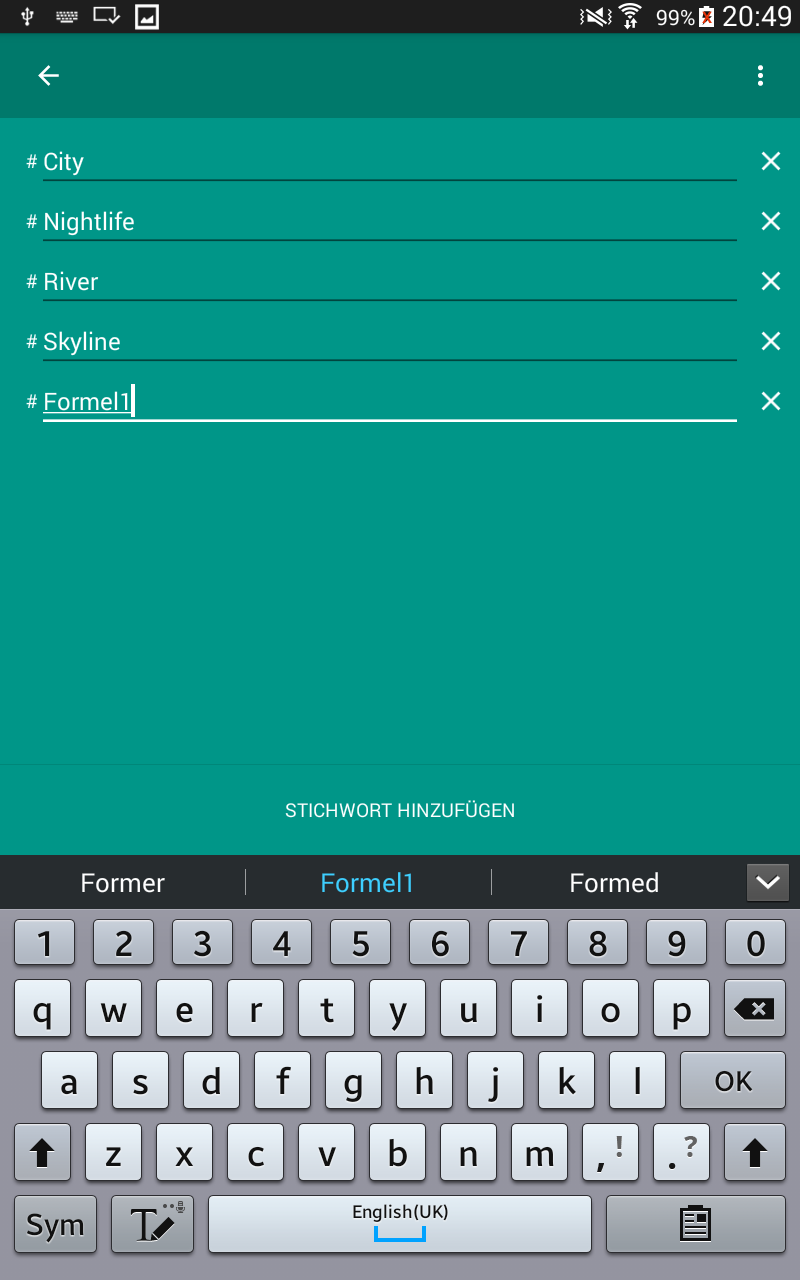
\includegraphics[height=20cm]{img/note_tagOverview}\\ % Pfad
\source{Screenshot aus der Benutzeroberfläche} % Quelle
\end{minipage}
\end{figure}

Im oberen Bildschirmbereich ist die Toolbar zu sehen. Darunter findet sich der ListView, welcher dynamisch erweitert werden kann und zu Beginn mit den übergebenen Stichworten initialisiert wird. Auf der rechten Seite können die einzelnen Stichworte gelöscht werden.

Unten befindet sich der Button zum Hinzufügen von Stichworten. Dieser wird dabei stets am unteren Rand des Displays angezeigt und verschiebt sich mit der Tastatur nach oben, falls diese aufgeklappt wird.

Die Farben der Activity werden aus der Notiz, aus welcher der Aufruf erfolgt ist, übernommen. Die Toolbar ermöglicht das Zurückkehren zur Notiz sowie das Löschen aller Stichworte über das Menü.

\paragraph{Use-Case (Joscha Nassenstein)}
Der Use-Case dieser Activity besteht darin, die Stichwortliste umfassend bearbeiten zu können. Die Möglichkeiten wurden dabei bereits in dem vorangegangenen Kapitel Aufgabe und Funktion dargestellt. 

\begin{figure}[H]
\centering
\begin{minipage}[t]{1\textwidth} % Breite, z.B. 1\textwidth		
\caption{NoteTag Use-Case Diagramm} % Überschrift
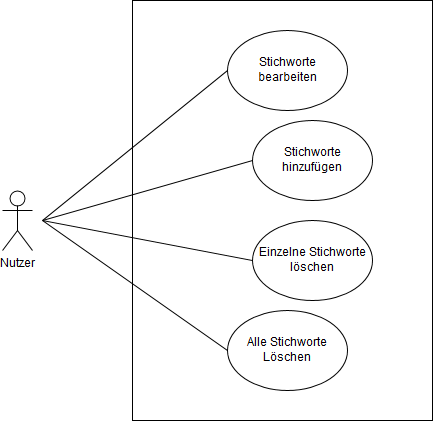
\includegraphics[width=1 \textwidth]{img/noteTagsUseCase}\\ % Pfad
\source{Erstellt von Joscha Nassenstein} % Quelle
\end{minipage}
\end{figure}

\paragraph{Datenstruktur und -typen (Joscha Nassenstein)}
Da die NoteTag-Activity nur einen sehr kleinen Umfang hat und deshalb nur wenige Klassen besitzt, wurde hier auf eine Unterstrukturierung in Packages verzichtet. Die Struktur orientiert sich an der in der Vorlesung vorgestellten Aufteilung. Alle Klassen mit Ausnahme der NoteTagActivity-Klasse sind dabei package-private, damit von außerhalb des Paketes nicht darauf zugegriffen werden kann.

\paragraph{Dokumentation des Quelltextes der Activity (Joscha Nassenstein)}
Im Nachfolgenden sind die einzelnen Klassen der NoteTag-Activity mit den jeweiligen wichtigsten Funktionen kurz beschrieben.

\subparagraph{Klasse: NoteTagActivity}
Diese Klasse ist der zentrale Einstiegspunkt der NoteTag-Activity und ist aus der AppCompatActivity-Klasse abgeleitet. Hier werden einige Methoden letzterer überschrieben und an die eigenen Anforderungen angepasst.

\textit{onCreate}:\\
In dieser Methode werden die über den Intent übergebenen Informationen, darunter die Stichwortliste, die Farbe und die Akzentfarbe, ausgelesen und mithilfe dieser die ApplicationLogic initialisiert. Zusätzlich wird die Gui-Klasse initialisiert.

\subparagraph{Klasse: ApplicationLogic}
Die ApplicationLogic-Klasse beinhaltet die Logik der NoteTag-Activity. Zusätzlich ist hier die ArrayList mit den Stichwörtern beinhaltet, da dies die einzigen Daten sind, welche für die NoteTag-Activity gehalten werden müssen und eine dedizierte Data-Klasse dafür zu viel Overhead produzieren würde.

\textit{returnToNoteActivity}:\\
In dieser Methode wird der Intent gebildet, welche als Result für die Activity gesetzt wird, damit dieser bei Abschluss der Activity an die NoteActivity übergeben wird. Zunächst werden dafür alle leeren Felder aus der Stichwortliste gelöscht und anschließend die Liste zum Intent hinzugefügt.

\textit{onDeleteButtonClicked}:\\
Hier wird anhand der übergebenen ID das entsprechende Stichwort gelöscht, der Adapter für den ListView benachrichtigt und anschließend die Tastatur ausgeblendet, falls diese eingeblendet war.

\textit{onTextChanged}:\\
Hier wird der übergebene Wert anhand der ID des Views, in welchem der Text geändert wurde, in die Stichwortliste eingefügt.

\textit{addInputTagField}:\\
In dieser Methode wird ein leerer String an die Stichwortliste angefügt und anschließend der Adapter benachrichtigt, sodass ein neues Feld für die Benutzereingabe erscheint.

\textit{onMenuItemClick}:\\
Diese Methode wird aufgerufen, falls der Benutzer im Toolbarmenü die Option „Alle Stichworte löschen“ ausgewählt hat. Hier wird die Liste der Stichworte geleert und anschließend zur Note-Activity zurückgekehrt. Eine weitere Abfrage ist hier nicht implementiert, da für das Löschen aller Stichworte so schon zwei Klicks nötig sind.

\subparagraph{Klasse: ClickListener}
Die Klasse ClickListener implementiert das Interface View.OnClickListener und kann dementsprechend auf ein View gesetzt werden, um die Benutzereingabe zu erkennen und Aktionen durchzuführen.

\textit{onClick}:\\
Hier wird überprüft, auf welchem View das Klick-Event ausgelöst wurde. Zur Auswahl stehen dabei der Zurück-Button der Toolbar, der Button, um ein Stichwort hinzuzufügen, sowie die einzelnen Entfernen-Buttons innerhalb des Listviews für jedes Stichwort. Je nach Ort der Ausführung wird die entsprechende Methode innerhalb der ApplicationLogic ausgeführt.

\subparagraph{Klasse: Gui}
Die Gui-Klasse beinhaltet die Benutzeroberflächenelemente als Attribute, wodurch auf diese zugegriffen werden kann. 

\textit{initiateListView}:\\
In dieser Methode wird der als Parameter übergebene ListViewAdapter auf den ListView gesetzt.

\textit{hideKeyboard}:\\
Hier wird das SoftKeyboard ausgeblendet.

\subparagraph{Klasse: ListViewAdapter}
Die Klasse ListViewAdapter erweitert ArrayAdapter<String> und kann dadurch auf einen ListView gesetzt werden.

\textit{getView}:\\
In dieser Methode wird eine Zeile des ListViews anhand des in den Layouts spezifizierten Zeilenlayouts initialisiert, die Position in der Liste als IDs auf die Views gesetzt und jeweils ein ClickListener für den Löschen-Button und ein TextWatcher für das Stichwort gesetzt. Anschließend wird der View zurückgegeben.

\subparagraph{Klasse: MenuItemClickListener}
Diese Klasse implementiert das Interface Toolbar.OnMenuItemClickListener und ist dafür zuständig, das Klicken auf ein Menüitem in der Toolbar, hier „Alle Stichworte löschen“, zu behandeln und dementsprechend hier die Methode in ApplicationLogic aufzurufen.

\subparagraph{Klasse: TextWatcher}
Der NoteTextWatcher implementiert das Interface android.text.TextWatcher und ist zur Speicherung von Eingaben in einem Stichwortfeld zuständig.

\textit{onTextChanged}:\\
Diese Methode überschreibt die entsprechende Methode der Basisklasse und ist dafür zuständig, die OnTextChanged-Methode in der ApplicationLogic aufzurufen, wo der Text in der ArrayList gespeichert wird.

\textit{afterTextChanged}:\\
In dieser Methode wird verhindert, dass die Texte Leerzeichen enthalten, da Stichworte immer als ein Wort geschrieben werden sollen.

\newpage
\fancyhead[L]{}
\subsection{Dokumentation der Navigation zwischen Activities (Yannick Rüttgers)}
%%%%%%%%%%%
%Yannick
%%%%%%%%%%%

Der Einstiegspunkt für den Nutzer ist die OverviewActivity. Von dieser aus können alle weiteren Activities aufgerufen werden, wie in der Planungsphase geplant.

Die Activities werden auf zwei Arten aufgerufen. Entweder geschieht dies, um ein neues TEN zu erstellen, oder um ein bereits vorhandenes aufzurufen.

Soll ein neues TEN erstellt werden, geschieht dies über einen der drei Buttons am oberen Bildschirmrand. Je nachdem welche TEN-Art angeklickt wurde, wird eine dazugehörige Activity erstellt und ohne Mitgabe weiterer Parameter aufgerufen.

Wenn hingegen ein bereits bestehendes TEN angezeigt werden soll, wird wieder die dazugehörige Activity erstellt. Diesmal wird der Activity allerdings als Parameter die ID des TENs weitergeben. Das Laden dessen übernimmt dann die jeweilige Activity.

Wenn aus den einzelnen TEN-Activities zurücknavigiert wird, gelangt der Nutzer zurück in die Übersichtsactivity. Die TENs innerhalb dieser werden neu geladen, um eventuelle Veränderungen anzeigen zu können.

\subsection{Dokumentation der Activity-übergreifenden, persistenten Datenhaltung (Jan Beilfuß)}
%%%%%%%%%%%
%Jan
%%%%%%%%%%%
\subsubsection{Persistente Datenhaltung}
\paragraph{Objekte}
Im Bereich der persistenten Datenspeicherung gab es die Herausforderung, dass es eine breite Auswahl an Speichermöglichkeiten gibt. Es musste zu Beginn evaluiert werden, welche Technologie für das Projekt am geeignetsten war. Zur Auswahl standen Bundles und Datenbanken, welche sich weiter in SQL-Datenbanken und NoSQL-Datenbanken unterteilen lassen. Darüber hinaus war zu Projektbeginn nicht bekannt, welche Datenbankimplementierungen für den Einsatz auf mobilen Geräten geeignet sind. Nach einiger Recherche wurde die Implementierung im Bundle als zu aufwendig und nicht flexibel genug erachtet. In der Folge wurde sich für den Einsatz einer Datenbank entschieden.

Aus dem bisherigen Studienverlauf waren unter den Datenbanken nur SQL-Datenbanken bekannt. Diese unterscheiden sich von NoSQL-Datenbanken, indem man eine klare Datenstruktur, in der Regel in Tabellenform vorgibt. NoSQL-Datenbanken sind beispielsweise dokumenten- oder graphenbasiert. Dokumente sind flexibel und diesen können einfach Felder in Form von Key-Value-Paaren hinzugefügt werden. Im mobilen Umfeld hat man häufig Änderungen am Datenmodell, sodass einem in diesem Bereich eine NoSQL-Datenbank entgegen kommt. Weiterhin hat man bei SQL-Datenbanken einen Aufwand zur Erzeugung und Definition von Tabellen sowie bei deren Änderung. Und da man aus den Anforderungen an die App ableiten konnte, dass keine komplexen Tabellenrechnungen gefordert waren, wurde sich für eine dokumentenbasierte NoSQL-Datenbank entschieden.

Bei der Wahl der spezifischen Datenbanktechnologie entschied man sich am Ende für Couchbase Lite, da diese gut dokumentiert ist, einem eine lokale Datenbank und Tools wie ein Gateway zur Hand gibt, wenn man es langfristig in Erwägung zieht Todos, Events und Notizen über einen Server zu synchronisieren.

Um den Aufwand bei der Umwandlung von Java-Objekten zu Dokumenten zu vereinfachen, wurde das Serialisierungs- und Deserialisierungsframework Jackson verwendet. Dieses wandelt Java Objekte in JSON-Strings um, welche in jeweils einem Dokument abgelegt wurden. Weiterhin bietet es eine Funktionalität, diese wieder zurückzuwandeln. Einige Attribute, darunter die ID des TEN-Objektes, die Hauptfarbe, die Kontrastfarbe und das Erzeugungsdatum wurden hiervon ausgenommen.

\begin{figure}[H]
\centering
\begin{minipage}[t]{1\textwidth} % Breite, z.B. 1\textwidth		
\caption{Dokumentenstruktur} % Überschrift
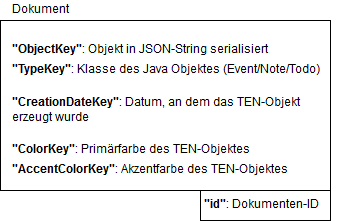
\includegraphics[width=10cm]{img/Dokumentenstruktur}\\ % Pfad
\source{Erstellt von Jan Beilfuß} % Quelle
\end{minipage}
\end{figure}

Die ID ist die ID des Dokumentes selber und würde somit doppelt gehalten werden. Die Farben wurden in eigenen Key-Value-Paaren abgelegt, damit man nicht das gesamte TEN-Objekt erzeugen muss, wenn man auf diese zugreifen möchte. Dies fand Einsatz in der Note Activity. Hier war es das Ziel die Performance beim Öffnen zu optimieren. Daher wurden die Farben getrennt von den eigentlichen Notizdaten im Vorraus geladen. Weiterhin wurde im Dokument gespeichert, welche Klasse das zuspeichernde Objekt hat, damit dieses beim Laden vernünftig aus dem JSON-String erzeugt werden kann. Zusätzlich wurden noch die Objektattribute welche bei Datenbankabfragen genutzt wurden, in einem eigenen Key-Value-Pair abgespeichert.

\paragraph{Bilder}
Das Speichern der Bilder hat sich im Vergleich zu den Java-Objekten als aufwendiger erwiesen, da diese mehr Speicherplatz und Rechenleistung benötigen.

Der erste Lösungsansatz war, die Bilder als Binary Large Objects in der Datenbank abzulegen. Dies erwies sich als zu imperformant und umständlich, sodass entschieden wurde, die Bilder im Dateisystem des Gerätes zu speichern. Weiterhin wurde zwischen den Bildern in voller Auflösung und Bildern in Vorschaugröße unterschieden. Die Vorschaubilder werden in der Übersicht und Notiz-Activity eingebunden. Aufgrund der stärkeren Kompression und geringeren Auflösung können diese schneller geladen werden. Darüber hinaus ist es auf dem Zielgerät hardwarebedingt nicht möglich, mehrere Bilder in Originalgröße im Arbeitsspeicher zu halten.

\subsubsection{Repository}
Das Repository bildet in der Applikationsstruktur die unterste Ebene und ist für das Handling der Datenbank und die Bereitstellung der persistent gespeicherten Daten verantwortlich.

\begin{figure}[H]
\centering
\begin{minipage}[t]{1\textwidth} % Breite, z.B. 1\textwidth		
\caption{Paketstruktur in der Repository-Schicht} % Überschrift
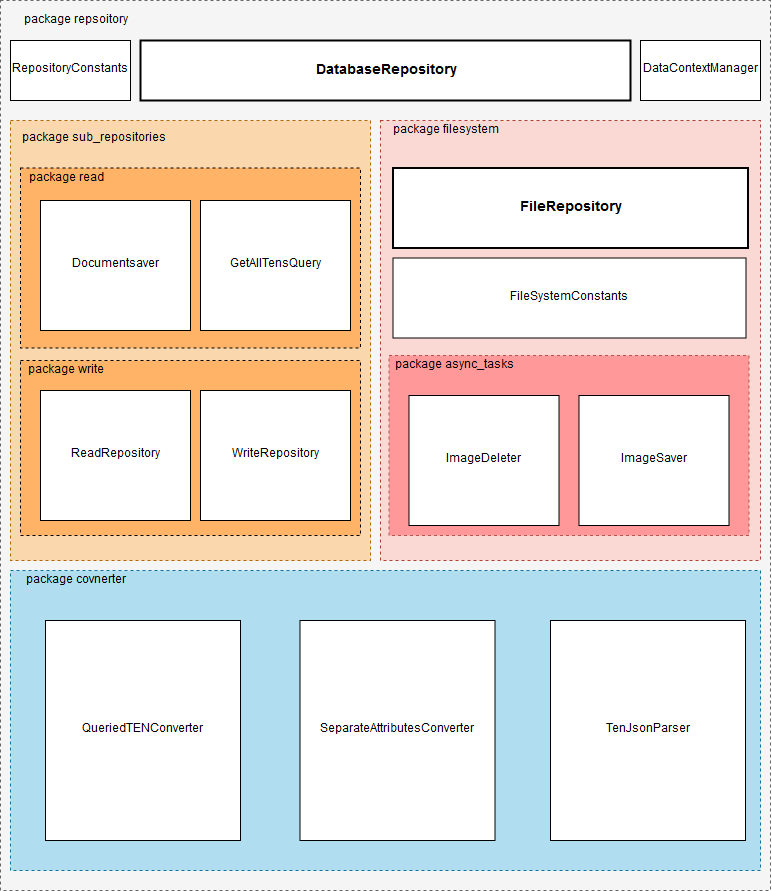
\includegraphics[width=1 \textwidth]{img/RepositoryPackages}\\ % Pfad
\source{Erstellt von Jan Beilfuß} % Quelle
\end{minipage}
\end{figure}

\paragraph{Klassenstruktur}

\subparagraph{Klasse: DatabaseRepository (Jan Beilfuß)}
Diese Klasse wird aus der Service-Schicht angesprochen. Sie bündelt Methoden, um Daten aus der Datenbank zu lesen oder in diese zu schreiben. Alle Methoden rufen Methoden in den Klassen WriteRepository oder ReadRepository auf.

\textit{ getTodoByID}:\\
Diese Methode gibt das zu der ID passende und in der Datenbank abgespeicherte Todoobjekt zurück. 

\textit{ getEventByID }:\\
Diese Methode gibt das zu der ID passende und in der Datenbank abgespeicherte Eventobjekt zurück. 

\textit{ getNoteByID }:\\
Diese Methode gibt das zu der ID passende und in der Datenbank abgespeicherte Noteobjekt zurück. 

\textit{ insertTEN }:\\
Diese Methode speichert ein neues TEN-Objekt in die Datenbank.

\textit{ updateTEN }:\\
Diese Methode aktualisiert ein bereits bestehendes TEN-Objekt.

\textit{ getAllTENs }:\\
Diese Methode gibt eine Liste aller in der Datenbank liegenden TEN-Objekte zurück.

\textit{ deleteTEN }:\\
Diese Methode löscht das in der Datenbank liegende Objekt zu der übergebenen ID.

\textit{ getTENColors }:\\
Diese Methode gibt die Haupt- und die Akzentfarbe des zu der übergebenen ID passenden TEN-Objektes zurück.

\subparagraph{ Klasse: DataContextManager (Jan Beilfuß)}
Diese Klasse managt das Handling des Datenbankenobjektes.

\textit{ initDatabase }:\\
Diese Methode prüft, ob die Datenbank mit dem übergebenen Datenbanknamen auf dem Gerät liegt. Falls dies der Fall ist wird diese als Datenbankobjekt in die Applikation geladen. Andernfalls wird eine neue erzeugt.

\textit{ compactDatabase }:\\
Diese Methode räumt die Datenbank auf. Da gelöschte Dokumente nur mit einem Flag versehen, aber nicht entgültig gelöscht werden, verbrauchen diese weiterhin Speicherplatz.

\textit{ getNumberOfDocuments }:\\
Diese Methode gibt die Anzahl der Datensätze zurück. Sie findet bei der Arbeit mit Mockdaten ihre Anwendung. Dadurch wird verhindert, dass diese mehrfach in die Datenbank geschrieben werden.

\textit{ getDatabase }:\\
Diese Methode gibt das Datenbankobjekt zurück.

\subparagraph{Klasse: RepositoryConstants (Jan Beilfuß)}
Diese Klasse enthält alle Konstanten, die bei der Arbeit mit der Datenbank benötigt werden. Dazu zählen die in den Dokumenten eingesetzten Schlüssel, aber beispielsweise auch der Name der Datenbank.

\subparagraph{Klasse: WriteRepository (Jan Beilfuß)}
Diese Klasse beinhaltet alle Funktionen, die einen schreibenden Zugriff auf die Datenbank haben. 

\textit{ insertTEN }:\\
Diese Methode erzeugt eine neues veränderbares Dokument und setzt in dem übergebenen TEN-Objekt die ID des Dokumentes. Dieses Dokument wird inklusive dem übergebenen TEN-Objekt dem DocumentSaver übergeben.

\textit{ updateTEN }:\\
Diese Methode lädt das Dokument aus der Datenbank und entfernt den Schreibschutz von diesem. Dieses Dokument wird inklusive dem übergebenen TEN-Objekt dem DocumentSaver übergeben.

\textit{ deleteTEN }:\\
Diese Methode lädt das zu der übergebenen ID passende Dokument aus der Datenbank. Weiterhin wird \textit{deleteNoteImages} aufgerufen, um die Bilder zu dem geladenen zu löschenden Objekt auch persistent zu löschen. Wenn ein Dokument zu der übergebenen ID existiert, wird dieses gelöscht.

\textit{ deleteNoteImages}:\\
Diese Methode entfernt alle mit dem zu löschenden Objekt assoziierten Bilder aus dem persistenten Speicher, sofern das zu löschende Objekt ein Note-Objekt ist.

\subparagraph{Klasse: DocumentSaver (Jan Beilfuß)}
Diese Klasse enthält alle Methoden, welche benötigt werden, um die Attribute eines TEN-Objektes in ein Dokument zu übertragen und dieses in der Datenbank zu speichern.

\textit{ updateCompleteDocument }:\\
Diese Methode wird aus dem WriteRepository aufgerufen und bildet den ganzen Prozess von der Dokumentenvorbereitung über das Hinzufügen der einzelnen Key-Value-Paare bis hin zum finalen speichern des Dokumentes ab.

\textit{ saveSeparateAttributes }:\\
Diese Methode legt alle Attribute, welche in der Serialisierung durch Jackson nicht beachtet warden, als Key-Value-Paare im Dokument ab. Dazu zählt unter anderem das Erzeugungsdatum des TEN-Objektes, die Farbe und die Akzentfarbe.

\textit{ setTypeOfDocument }:\\
Diese Methode bestimmt abhängig von der Klasse des übergebenen TEN-Objektes, welcher Typ in dem Dokument gespeichert werden muss. Dies ist notwendig, da bei der Deserialisierung des JSON-Strings, die Zielklasse angegeben werden muss.

\subparagraph{Klasse: ReadRepository (Jan Beilfuß)}
Diese Klasse beinhaltet alle Methoden, die einen lesenden Zugriff auf die Datenbank haben.

\textit{ getTodoByID }:\\
Diese Methode lädt ein einzelnes Dokument aus der Datenbank und wandelt dieses in ein Todo-Objekt um. Dazu wird erst aus dem JSON-String das Objekt erzeugt und im Anschluss die separat abgelegten Attribute gesetzt.

\textit{ getEventByID }:\\
Diese Methode lädt das zu der übergebenen ID passende Dokument aus der Datenbank und wandelt dieses in ein Event-Objekt um. Dazu wird erst aus dem JSON-String das Objekt erzeugt und im Anschluss die separat abgelegten Attribute gesetzt.

\textit{ getNoteByID }:\\
Diese Methode lädt das zu der übergebenen ID passende Dokument aus der Datenbank und wandelt dieses in ein Note-Objekt um. Dazu wird erst aus dem JSON-String das Objekt erzeugt und im Anschluss die separat abgelegten Attribute gesetzt.

\textit{ getAllTENs }:\\
Diese Methode ruft die Query getAllTENs auf und gibt dann das Ergebnis dieser, eine Liste aller in der Datenbank gespeicherten TEN-Objekte, zurück.

\textit{ getTENColors }:\\
Diese Methode lädt das Dokument zu der übergebenen ID aus der Datenbank und gibt die Haupt- und die Akzentfarbe des erzeugten TEN-Objektes zurück.
\subparagraph{Klasse: GetAllTensQuery (Jan Beilfuß)}
Diese Klasse enhält die Datenbankabfrage, um alle TEN-Objekte aus der Datenbank zu laden.

\textit{ getAllTENs }:\\
Diese Methode baut eine Datenbankabfrage, um alle TEN-Objekte aus der Datenbank zu laden. Die Einträge des ResultSets werden dem entsprechenden Converter übergeben, dort umgewandelt und dann einer Liste aus TEN-Objekten hinzugefügt, welche am Ende zurückgegeben wird.

\subparagraph{Klasse: QueriedTENConverter (Jan Beilfuß)}
Diese Klasse enthält eine Methode, welche genutzt wird, um die Ergebnisse einer Datenbankabfrage in TEN-Objekte umzuwandeln.

\textit{ createTENFromResult }:\\
Diese Methode wandelt ein Result, eine CouchbaseLite-Klasse, in ein TEN-Objekt um. Dem Result wird ein Dictionary entnommen und aus diesem der JSON-String. Der wird im Anschluss zur Erzeugen des TEN-Objektes verwendet. Wenn dies erfolgreich ist, werden dem TEN-Objekt noch die separat abgelegten Attribute hinzugefügt.

\subparagraph{Klasse: SeparateAttributesConverter (Jan Beilfuß)}
Diese Klasse ist dafür verantwortlich, dass in einem übergebenen TEN-Objekt die nicht im JSON-String enthaltenen Attribute gesetzt werden. Dazu zählt die ID, welche die ID des Dokuments selber ist, die Hauptfarbe, die Akzentfarbe und das Erzeugungsdatum des TEN-Objektes.

\textit{ addTENPropertiesFromDocument }:\\
Diese Methode entnimmt die aufgeführten Attribute einem Document, Objekt aus dem Couchbase Lite-Umfeld, und setzt diese im übergebenen TEN-Objekt.

\textit{ addTENPropertiesFromResult }:\\
Diese Methode entnimmt die aufgeführten Attribute einem Result, Objekt aus dem Couchbase Lite-Umfeld, und setzt diese im übergebenen TEN-Objekt.

\subparagraph{Klasse: TenJsonParser (Jan Beilfuß)}
Diese Klasse enthält Methoden, die aus einem JSON-String die TEN-Objekte erzeugen. Dafür wird das Framework Jackson eingesetzt.

\textit{ stringToTodo }:\\
Diese Methode erzeugt aus dem übergebenen JSON-String ein Todo-Objekt und gibt dieses zurück.

\textit{ stringToEvent }:\\
Diese Methode erzeugt aus dem übergebenen JSON-String ein Event-Objekt und gibt dieses zurück.

\textit{ stringToNote }:\\
Diese Methode erzeugt aus dem übergebenen JSON-String ein Note-Objekt und gibt dieses zurück.

\subparagraph{Klasse: FileRepository (Jan Beilfuß)}
Diese Klasse enthält alle Zugriffe auf das Dateisystem. Sie findet Einsatz in der Verwaltung der Bilder, da diese im Dateisystem abgelegt werden.

\textit{ saveImagePersistent }:\\
Diese Methode erzeugt ein Objekt der Klasse ImageSaver und speichert darüber das übergebene Bild im Dateisystem.

\textit{ readImageFromDirectory }:\\
Diese Methode ist dafür verantwortlich, aus einem Image-Objekt mit leerer Bitmap und dem übergebene Ordnernamen, das entsprechende Bild zu laden. Dafür baut man aus einem Grundpfad, dem übergebenen Ordnernamen und der im Image-Objekt enthaltenen ID den Bildpfad zusammen. Im Anschluss wird die zu dem Pfad gehörende Datei zu einer Bitmap dekodiert, ein neues Image-Objekt inklusive der Bitmap erzeugt und dieses zurückgegeben.

\textit{ deleteImageFromDirectory }:\\
Die Methode deleteImageFromDirectory überladen. Diese nimmt den absoluten Pfad einer Datei an und löscht diese, falls sie existiert. Diese Methode ist synchron, da sie lediglich für einzelne Dateien beim Kameraimport verwendet wird und sich innerhalb eines vernachlässigbaren Bereichs auf die Performance auswirkt.

\textit{ deleteImageFromDirectory }:\\
Die Methode deleteImageFromDirectory überladen. Diese nimmt ein Image-Objekt an und erzeugt einen ImageDeleter. Diese Klasse erzeugt einen asynchronen Task, um das Bild zu löschen. Hier wird asynchron gearbeitet, da diese Methode beim Schließen der Notiz-Activity aufgerufen wird, um alle zuvor als zu löschend markierten Bilder zu löschen. Da eine flüssige Navigation gewährleistet werden soll, wird hier der UI-Thread verlassen.

\subparagraph{Klasse: FileSystemConstants (Jan Beilfuß)}
Diese Klasse enthält alle Konstanten, welche im Umgang mit dem Filesystem benötigt werden. Dazu zählen Ordernamen, Dateiendungen, aber auch der Kompressionsfaktor für Bilder.

\subparagraph{Klasse: ImageDeleter (Jan Beilfuß)}
Diese Klasse erzeugt einen asynchronen Task, der die Bilder aus dem Dateisystem löscht. Diese Klasse enthält als innere Klasse die Klasse DeleteImageTask, welche von AsyncTask erbt.

\textit{ execute }:\\
Es wird ein asynchroner Task der Klasse DeleteImageTask erzeugt und ausgeführt. Dieser löscht die Bilder zu der im ImageObjekt übergebenen ID. Die dort definierte Methode \textit{doInBackground} baut die Dateipfade für die beiden Ordner Originale Bilder und Vorschaubilder zusammen, überprüft, ob die Datei existiert und löscht diese, falls sie existiert.

\subparagraph{Klasse: ImageSaver (Jan Beilfuß)}
Diese Klasse erzeugt einen asynchronen Task, der die Bilder im Dateisystem speichert. Diese Klasse enthält als innere Klasse die Klasse SaveImageTask, welche von AsyncTask erbt.

\textit{ execute }:\\
Es wird ein asynchroner Task der Klasse SaveImageTask erzeugt und ausgeführt. Die dort definierte Methode \textit{doInBackground} baut die Zielpfade für die beiden Ordner Originale Bilder und Vorschaubilder zusammen. Im Anschluss wird geprüft, ob das Bild bereits existiert, um diese nicht bei jedem Speichern zu überschreiben. Wenn die übergebene Bitmap nicht Null ist wird diese über ein Objekt der Klasse FileOutputStream dort abgelegt. Für den Ordner der Vorschaubilder wird zuvor ein Vorschaubild erzeugt, und dieses abgespeichert.

\newpage
\subsection{Dokumentation der Activity-übergreifenden Klassen}
%%%%%%%%%%%
%Ruthild
%%%%%%%%%%%

Zu den Activity-übergreifenden Klassen gehören abgesehen von den Repository-Klassen für die persistente Datenhaltung auch die Service-Klassen und die Models-Klassen. Die Models-Klassen enthalten die TEN-Klasse und die einzelnen Todo-, Event- und Note-Klassen. Hier sind auch weitere Util-Klassen untergeordnet. In den Service-Klassen sind Methoden enthalten, die die Schnittstelle zwischen Datenbank und Activities darstellen. Im Folgendem wird genauer auf die einzelnen Klassen eingegangen.

\begin{figure}[H]
\centering
\begin{minipage}[t]{1\textwidth} % Breite, z.B. 1\textwidth		
\caption{Übersicht über Data-Klassen} % Überschrift
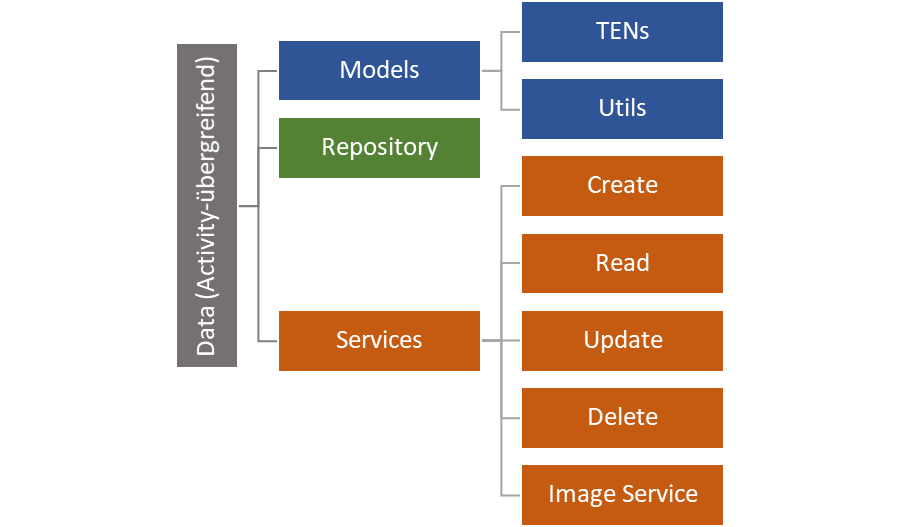
\includegraphics[width=1\textwidth]{img/StrukturDataKlassen}\\ % Pfad
\source{Erstellt von Ruthild Gilles} % Quelle
\end{minipage}
\end{figure}

\subsubsection{Models-Klassen (Ruthild Gilles)}

Wie schon während der Planungsphase definiert, gibt es Klassen, in denen die Struktur der einzelnen TEN-Objekte definiert ist. Sowohl die Todo-Klasse als auch die Event- und Note-Klasse erben von der TEN-Klasse. In dieser werden für alle TEN-Objekte Attribute wie der Titel, eine ID, ein Erstellungsdatum und die Farbe deklariert. Die Farbe wird dabei bei Initialisierung eines Objektes zufällig aus einer Liste von Farben ausgewählt. Die Farben wurden anhand eines Material-Designs ausgewählt, damit die graphische Benutzeroberfläche ästhetisch ansprechend ist und sich keine Farben beißen.

Die Klassen für die einzelnen Objekt-Typen enthalten weitere Attribute, die notwendig sind, um alle relevanten Informationen darstellen zu können.

In der Klasse Todo werden zusätzlich noch Attribute für den Fortschritt der Erfüllung des Todos, einer Notiz, eines Start- und Enddatums deklariert. Der wichtigste Teil eines Todo-Objektes ist die Liste an Aufgaben, die abgearbeitet werden sollen. Dazu wurde eine weitere Klasse implementiert, welche die Struktur einer einzelnen Aufgabe angibt. Aufgaben bestehen aus einer Beschreibung und einem binären Status. Objekte dieser Klasse können in einem Objekt der Klasse Todo in einer ArrayList gespeichert werden.

Die Klasse Event erweitert das TEN-Objekt noch um ein Datum inklusive Uhrzeit, eine Adresse und ein Wiederholungstyp. Dieser kann folgende Werte annehmen: None, Daily, Weekly, Monthly oder Yearly. Die Werte sind in einem Enum im Ordner Utils definiert. Zusätzlich können einem Event-Objekt mehrere Erinnerungen hinzugefügt werden. Diese werden ähnlich wie die Aufgaben eines Todo-Objektes in einer ArrayList gesammelt.

Ein Note-Objekt enthält, abgesehen von den Attributen aus der TEN-Klasse, zusätzlich eine Beschreibung, mehrere Tags und Bilder, welche in ArrayListen dem Note-Objekt hinzugefügt werden können. Ein Bild ist ein Objekt der Bild-Klasse und enthält die Attribute ID und Bitmap.

Damit für die Präsentation der Applikation bereits einige Todo-, Event- und Note-Objekte in der Benutzeroberfläche zu sehen sind, gibt es eine weitere Klasse, welche Mockdaten initialisiert. Diese werden auf die Datenbank geschrieben und von dort wie reguläre Daten verwendet.

\subsubsection{Service-Klassen (Ruthild Gilles)}

Damit die Activities die Daten der TEN-Objekte auf der dokumentenbasierten Datenbank speichern können, wurden Service Klassen implementiert. Hierzu gehörten hauptsächlich Klassen zum Erzeugen neuer TEN-Objekte (Create), zum Erhalten bereits gespeicherter TEN-Objekte von der Datenbank (Read), zum Speichern veränderter TEN-Objekte (Update) und zum Löschen von TEN-Objekten von der Datenbank (Delete). Diese sogenannte CRUD-Operationen wurden in den entsprechenden Klassen teilweise für alle drei verschiedenen Objekttypen einzeln eingefügt, teilweise aber auch für TEN-Objekte im Allgemeinen. Dank Polymorphie können die jeweils einzelnen Objekttypen ebenfalls an die entsprechenden Methoden übergeben werden.

Diese Struktur wurde während der Planungsphase vom Datenteam überlegt und während der Implementierung angepasst. Wie auch schon in der Planungsphase definiert enthält die Create-Klasse Methoden, die ein neues leeres Todo, Event oder Note zurückgeben. Diese Methode ruft den Konstruktor der jeweiligen TEN-Klasse auf. Eine Interaktion mit der Datenbank ist hier noch nicht nötig.

Die Read-Klasse hingegen muss auf die Datenbank zugreifen, um entweder alle TEN-Objekte an die Main-Activity in einem ListArray zu übergeben oder aber ein spezielles Todo, Event oder Note, welches von den einzelnen Todo-, Event- oder Note-Activities aufgerufen werden kann. Damit das gewünschte TEN-Objekt in der Datenbank gefunden werden kann, benötigen die Read-Methoden die ID des gewünschten Objektes. Dieses wird als String beim Aufruf der jeweiligen Methode übergeben.

Die Update-Klasse dient zum Speichern von Änderungen an Todo-, Event- und Note-Objekten. Dazu überprüft die Methode, der ein TEN-Objekt übergeben wurde, ob dieses bereits auf der Datenbank existiert. Ist dies der Fall, wird eine Methode zum Ausführen des Update-Befehls auf der Datenbank aufgerufen. Ist dies nicht der Fall, wird eine Methode zum Ausführen des Insert-Befehls auf der Datenbank aufgerufen. Da die Todo-, Event- und Note-Klassen von der TEN-Klasse erben, kann hier Polymorphie angewandt werden. Es ist nur eine Methode zum Speichern notwendig.

Für das Löschen von TEN-Objekten sind in der Delete-Klasse zwei Methode vorhanden. Die eine löscht nur ein übergebenes TEN-Objekt aus der Datenbank, indem es eine entsprechende Methode aus einer der Repository-Klassen aufruft und dieser die ID des TEN-Objektes übergibt. Sollen jedoch mehrere TEN-Objekte auf einmal gelöscht werden, kann der zweiten Methode eine Array List, die mehrere zu löschende Objekte enthält, übergeben werden. Dabei müssen die Objekte nicht alle von dem gleichen Datentyp sein, sondern können Todo-, Event- und Note-Objekte enthalten. Die Methode iteriert durch die übergebene Array List und ruft für jeden Eintrag die Methode zum Löschen eines Objektes auf.

In den Service Klassen bestehen zusätzlich zwei Klassen für die Verarbeitung von Bildern.

Die Klasse ImageService stellt dabei Funktionen für die Schnittstelle zur Datenbank zur Verfügung, beispielsweise zum Laden oder Löschen eines Bildes. Zusätzlich kann eine temporäre Bilddatei zur Übergabe an den Kamera-Intent erstellt werden, in welcher bei der Aufnahme die Bilddatei gespeichert wird. Die Klasse ImageCorrectionService stellt Funktionen zur Korrektur der Ausrichtung eines Bildes anhand der mitgelieferten Exif-Daten bereit, da auf einigen Geräten die Bilder sonst nicht korrekt dargestellt wurden. Diese Klassen werden zurzeit lediglich von der Note-Activity genutzt.

\subsubsection{Modules-Klassen}
\paragraph{Paket: modules}
In diesem Paket werden Funktionen gebündelt, die in mehrere Activities implementiert werden oder das Potenzial dazu haben. 
\subparagraph{Paket: image}

\subparagraph*{Klasse: ImageToolsModule (Jan Beilfuß)}
Diese Klasse bündelt die Methoden, welche im Modul ImageTools enthalten sind und dient bei Aufrufen aus den Activities als Single Point Of Contact.

\textit{ importCompressedImage }:\\
Dieser Methode wird der Pfad zu einer Bilddatei übergeben. Sie ruft die Methode \textit{importCompressedImage} im ImageCompressionModule auf, welche die Bitmap zurückgibt, welche auf dem Pfad liegt.

\textit{ correctImageRotation }:\\
Dieser Methode wird der Pfad zu einer Bilddatei und die dazugehörige Bitmap übergeben. Sie ruft die Methode \textit{corretImageRotation} im ImageCompressionModule auf, welche die Bitmap abhängig von dem Bild zu Pfad dreht und zurückgibt.

\subparagraph*{Klasse: ImageCompressionModule (Jan Beilfuß)}
Diese Klasse bündelt die Methoden, welche benötigt werden, um Bilder komprimiert aus dem Dateisystem zu importieren.

\textit{importCompressedImage}:\\
In den BitmapFactory.Options kann man einen Wert setzen, sodass beim Dekodieren nur die Informationen zu dem Bild eingelesen werden. Dazu zählt unter anderem auch die Höhe und die Breite. Diese wird dann genutzt, um einen Skalierungsfaktor zu berechnen, um die Größe des Bildes auf den Arbeitsspeicher des Zielgerätes anzupassen. Dieser wird beim Dekodieren der Bilddatei berücksichtigt, sodass ein kleineres Bild mit weniger Speicherverbrauch in den Arbeitsspeicher geladen wird.

\textit{calculateImportSampleSize}:\\
Diese Methode berechnet den Skalierungsfaktor, welcher benötigt wird, um das Bild von der Originalgröße auf die kleinste Größe oberhalb der Zielgröße zu bekommen. Dabei ist zu beachten, dass der Faktor eine Zweierpotenz ist, da auf diese abgerundet wird. Der Faktor wird schrittweise erhöht. Sobald das Bild kleiner als die Zielgröße ist, wird der Faktor zurückgegeben.

\subparagraph*{Klasse: ShareModule (Fabia Schmid)}
Das ShareModule bietet jeweils für Todo, Event und Note eine Funktion, welche angesprochen werden kann, um den jeweiligen Inhalt in einer externen App zu teilen. Dafür wird ein Intent erstellt, welcher einen Benutzerdialog startet, in dem ausgewählt werden kann, in welcher Form beziehungsweise in welcher Applikation der Inhalt geteilt werden soll. Innerhalb des Intents werden anschließend die Felder Betreff und Text mit den entsprechenden Daten aus dem momentan geöffneten TEN-Objekt gefüllt. Die Struktur des Textes entspricht dabei der Struktur eines Todos, eines Events oder einer Notiz. Anschließend wird die Activity zum Anzeigen des Dialoges und dem anschließenden Teilen gestartet.




